\ProvidesFile{chapters/ch-Event_Selection.tex}

\chapter{Datasets, Event Selection, and \ensuremath{\mathrm{t\bar{t}}} Kinematic Reconstruction}
\label{Datasets_Event_Selection_Kinematic_Reconstruction}
The signal process for this measurement is the production of top quark pairs followed by top quark decays $t\to W^+ b$ and $\bar{t}\to W^- \bar{b}$, and subsequent leptonic $W$ boson decays into final state muons $W\to \mu\nu$ and electrons $W\to e\nu$, both "prompt" and "via tau", i.e. via the decay of the W boson into a tau $W\to \tau\nu$ and its subsequent leptonic decay into a final state electron $\tau\to e\nu$ or muon $\tau\to \mu\nu$.
The analysis has been carried out using the CMS EDM and official software framework for event generation, simulation, and reconstruction, following recommendations for ultra-legacy Run II analyses by the Physics Performance and Datasets (PPD) and the Physics Data And Monte Carlo Validation (PdmV) CMS groups.

\section{Datasets}

\subsection{Recorded Datasets}
This measurement is performed using \lumivalueSixPreVFP $\pm$ \lumierrSixPreVFP~\cite{bib:lumipas16}, \lumivalueSixPostVFP $\pm$ \lumierrSixPostVFP~\cite{bib:lumipas16}, \lumivalueSeven $\pm$ \lumierrSeven~\cite{bib:lumipas17}, and \lumivalueEight $\pm$ \lumierrEight~\cite{bib:lumipas18} (Total: \lumivalueRuniiUL $\pm$ \lumierrRuniiUL) of data collected with the CMS experiment at the LHC with \beamenergy, during 2016, 2017, and 2018 respectively.
Only the runs and luminosity sections that had good functioning of every CMS sub-detector were selected for analysis.

\subsection{Simulated Datasets}
MC simulations are used to estimate signal and background contributions. 
The dileptonic \ttbar signal sample is produced using the \Powheg\ event generator with NLO ME calculations. 
PS and hadronization of the \ttbar signal sample is performed using \Pythia. 
The matrix-element jets are matched to parton showers using the \Powheg\ method. 
The MC simulations assume that $m_t = \SI{172.5}{\GeV}$, and the PDFs are described using NNPDF3.1.
\Powheg\ assumes that the \ttbar branching fractions are flavor-independent with flavor-averaged branching fractions of $0.1091$, so correction factors were calculated and applied to correct each dilepton channel to the flavor-specific PDG value.
The following flavor-specific branching fractions are taken from PDG~\cite{bib:PDG}: $b_{{\ensuremath{W\to e\nu}}} = 0.1071$ $\pm$ 0.0016, $b_{{\ensuremath{W\to \mu\nu}}} = 0.1063$ $\pm$ 0.0015, and $b_{{\ensuremath{W\to \tau\nu}}} = 0.1138$ $\pm$ 0.0021.
The branching fraction of $\tau$ leptons decaying into a muon is given by $b_{{\ensuremath{\tau\to \mu\nu\nu}}} = 0.1741$ $\pm$ 0.0004 and for taus decaying to an electron it is $b_{{\ensuremath{\tau\to e\nu\nu}}} = 0.1783$ $\pm$ 0.0004.
The following \ttbar dilepton branching fraction global correction factors were applied per prompt dilepton channel: $\mathcal{C}_{\ee} = 0.9643$, $\mathcal{C}_{\emu} = 0.9571$, and $\mathcal{C}_{\mumu} = 0.9499$.  
\ttbar dilepton events with at least one leptonic tau decay are considered as signal in this analysis and the following branching fraction global correction factors were applied per dilepton channel via tau: $\mathcal{C}_{\ee} = 1.0298$, $\mathcal{C}_{\emu} = 1.0262$, and $\mathcal{C}_{\mumu} = 1.0227$.

The major sources of background contributions are semi-leptonic \ttbar, fully hadronic \ttbar, dileptonic decays of single top quarks in association with a $W$ boson ($tW$ and $\bar{t}W$), \ttbar in association with $W/Z$ bosons, \zjets, \wjets, and $WW$, $WZ$, $ZZ$ diboson processes. 
A summary of the MC simulated process for background processes is shown in table~\ref{simulated_Datasets}, including the ME generator, PS algorithm, and cross-section used for luminosity scaling.

\begin{table}[!htb]
 \begin{center}
   \begin{adjustbox}{scale=0.75,center}
    \begin{tabular}
      {lccr} \hline Process & ME (Matching) & PS & $\sigma$ [pb]\\
      \hline
      { \ttbar (Dileptonic)} & \Powheg & \Pythia &  $\xsecTTBARdilept$ \\
      { \ttbar (Semi-Leptonic)} & \Powheg & \Pythia &  $\xsecTTBARljets$ \\
      { \ttbar (Hadronic)} & \Powheg & \Pythia &  $\xsecTTBARhadronic$ \\
      { $\ttbar+W$ (Leptonic $W$)} & \MGaMCatNLOOnly+\MadSpin & \Pythia &  $\xsecTTWJETSlnu$ \\
      { $\ttbar+W$ (Hadronic $W$)} & \MGaMCatNLOOnly+\MadSpin & \Pythia &  $\xsecTTWJETSqq$ \\
      { $\ttbar+Z$ (Leptonic $Z$)} & \MG & \Pythia &  $\xsecTTZllnunu$ \\
      { $\ttbar+Z$ (Hadronic $Z$)} & \MG & \Pythia &  $\xsecTTZqq$ \\
      { $t+W$ (Dileptonic)} & \Powheg & \Pythia &  $\xsecSINGLETOPtw$ \\
      { $\bar{t}+W$ (Dileptonic)} & \Powheg & \Pythia &  $\xsecSINGLETOPtw$ \\
      { $W+\text{Jets}$} & \MG & \Pythia &  $\xsecWlnu$ \\
      { $Z/\gamma^*+\text{Jets} \quad (\SI{10}{\GeV} < m_{\ell\bar{\ell}} < \SI{50}{\GeV})$} & \MG & \Pythia &  $\xsecDYTenFifty$ \\
      { $Z/\gamma^*+\text{Jets} \quad (\SI{50}{\GeV} < m_{\ell\bar{\ell}})$} & \MG & \Pythia &  $0.5 \times \xsecDYFiftyInf$ \\
      { $Z/\gamma^*+\text{Jets} \quad (\SI{50}{\GeV} < m_{\ell\bar{\ell}})$} & \MGaMCatNLO & \Pythia &  $0.5 \times \xsecDYFiftyInf$ \\
      { $WW$} & \Pythia & \Pythia &  $\xsecWW$ \\
      { $WZ$} & \Pythia & \Pythia &  $\xsecWZ$ \\
      { $ZZ$} & \Pythia & \Pythia &  $\xsecZZ$ \\
      \hline
      \end{tabular}
   \end{adjustbox}
  \caption{}
  \label{simulated_Datasets}     
 \end{center}
\end{table}

\section{Event Selection and Object Corrections}
The \ttbar dilepton final state is characterized by the presence of at least two high-\pT isolated leptons with opposite electric charge, large MET (\ETmiss), and two jets created from the hadronization of $b$-quarks.
The reconstruction of the different objects is performed using the PF algorithm.
The object identification criteria follow the recommendations for ultra-legacy Run II analyses by the CMS Top Physics Analysis Group (Top PAG).

\subsection{Triggers}
To maximize the trigger efficiency, dilepton data streams and single lepton streams are both used for this measurement.
In order to ensure no double-counting of events, events passing the dilepton triggers are vetoed when processing the single lepton data streams.
Approximately 10\% of dilepton events that failed to pass the dilepton trigger requirements are recovered by including the single lepton data streams.
The trigger efficiency is measured in data as a function of the lepton $\pT$ and used to correct the MC simulations.

\subsection{Primary Vertex Requirements and Pileup Corrections}
The PV of an event is required to associated with at least four tracks and be in the vicinity of the nominal interaction point with $\vert r \vert < \SI{2}{\cm}$ and $\vert z \vert < \SI{24}{\cm}$. 
Charged-hadron subtraction (CHS) is used to remove charged PU contributions and the L1FastJet algorithm is applied to subtract the remaining neutral contributions.
The number of PU events in MC simulations is typically based on an estimate of the expected number of interactions per bunch crossing and PU reweighting is performed using the instantaneous luminosity per bunch crossing in data, and the total $pp$ inelastic cross section of $\SI{69.2}{\m \b}$, to correct the PU distribution of the MC simulation.

\subsection{Muons}
PF muon candidates are required to have a transverse momentum $\pT > \SI{20}{\GeV}$ and a pseudorapidity restricted to the coverage of the inner tracker $\vert \eta \vert < 2.4$.
They are also required to be reconstructed as global muons and fulfill tight selection criteria: 
\begin{itemize}
    \item at least six hits in the tracker layers
    \item at least one hit in the pixel detector
    \item muon segments in at least two muon stations
    \item at least one muon-chamber hit included in the global-muon track fit
    \item $\chi^2/ndof < 10$ for the global muon fit
    \item its track has transverse impact parameter $d_xy< \SI{2}{\mm}$ and longitudinal distance $d_z< \SI{5}{\mm}$ with respect to the primary vertex
\end{itemize}
These criteria suppress hadronic "punch-through" fake-muons and muons produced in hadron decays to ensure high purity and provide good $\pT$ measurements.
To remove leptons overlapping with jets, PF muon candidates are required to fulfill the isolation condition $I^{PF}_{Rel}< 0.15$, where $I^{PF}_{Rel}$ is calculated as: 
\begin{linenomath*}
\begin{align}
I^{PF}_{Rel} = \frac{1}{\pT(\mu)}(I_\mathrm{CH} + \max(0, I_\mathrm{N} + I_\mathrm{PH} - 0.5 I_\mathrm{CH,pu}))
\end{align}
\end{linenomath*}
and divided by the \pT of the muon.
It is the \pT-sum of charged (CH), neutral (N), and photon-like (PH) transverse energy deposits from charged hadron, neutral hadron and photon PF candidates, relative to the \pT of the muon, inside a cone, in $\eta$-$\phi$ space, of $\Delta R < 0.4$ around the muon.
$I_\mathrm{CH,pu}$ is the sum over charged PF candidates not originating from the main primary vertex and its subtraction compensates for PU contributions. 
Corrections are also applied that scale the raw energy measurements and smear the muon resolutions to match the accuracy and precision of reconstructed muons in MC simulation to those in recorded data.
Identification and isolation efficiency corrections for muons are also applied, and are measured as a function of \pT and $\eta$ using a "tag-and-probe" method with an orthogonal dataset.

\subsection{Electrons}
PF electron candidates are required to have transverse momentum $\pT > \SI{20}{\GeV}$ and a pseudorapidity restricted to the coverage of the inner tracker $\vert \eta \vert < 2.4$.
The gap between the barrel and endcap region of the ECAL ($1.4442 < \vert \eta_\mathrm{sc} \vert < 1.5660$) is excluded, where $\eta_\mathrm{sc}$ is the pseudorapidity of the ECAL supercluster.
To ensure high purity, the electron selection uses tight identification and isolation criteria.
The electron isolation considers photons $\gamma$, neutral hadrons $\mathrm{nh}$, and charged hadrons $\mathrm{ch}$ as identified by the PF algorithm in a cone, in $\eta$-$\phi$ space, of $\Delta R < 0.3$ around the electron.
The relative isolation is calculated as: 
\begin{linenomath*}
\begin{align}
I^{PF}_{Rel} = I_{\mathrm{ch}} + \max(I_\gamma + I_{\mathrm{nh}} - \rho A_{\mathrm{eff}}, 0)
\end{align}
\end{linenomath*}
and divided by the \pT of the electron.
$A_{eff}$ is an $\eta$ dependent effective area that gives information about the susceptibility to soft contamination and is chosen such that isolation is flat with respect to the number of PU interactions. 
It is used in combination with $\rho$, which is an estimate of the energy density per unit area contributed by PU interactions, to subtract energy deposition from PU interactions from the isolation.
$\rho$, the energy deposition per area due to unclustered objects, is estimated from the fixed grid approach and the $\rho A_{eff}$ term ensures that the isolation efficiency is almost independent of the PU conditions.
Corrections are also applied that scale the raw energy measurements and smear the electron resolutions to match the accuracy and precision of reconstructed electrons in MC simulation to those in recorded data.
Identification and reconstruction efficiency corrections for electrons are also applied, and are measured as a function of \pT and $\eta$ using a "tag-and-probe" method with an orthogonal dataset.

\subsection{Lepton Pair}
Events with a dilepton system consisting of exactly two oppositely-charged leptons passing the electron and muon object selection criteria are accepted for further consideration.
If more than two leptons are reconstructed in the event, then the event is vetoed.
The leading selected lepton is required to have $\pT > \SI{25}{\GeV}$.
The event is then unambiguously classified as \ee, \emu, or \mumu depending on the type of the selected lepton pair, and the event is discarded if there are additional leptons in the event, other than the two which enter the defined lepton pair.
The invariant mass of the selected lepton pair is required to be larger than $\SI{20}{\GeV}$ to suppress background events from decays of heavy-flavour resonances and Drell-Yan processes.
Moreover, in the \mumu and \ee decay channels, events are rejected if the dilepton invariant mass is within the vicinity of the $Z$ boson mass $\SI{76}{\GeV} < m_{\ell\bar{\ell}} < \SI{106}{\GeV}$, where background from $Z$ boson production is dominant.

\subsection{Jets}
Jets are clustered from reconstructed PF candidates using the anti-$k_T$ clustering algorithm with radius parameter $R = 0.4$ (AK4).
Events are required to have at least two jets with transverse momentum $\pT > \SI{30}{\GeV}$ and within the coverage of the inner tracker $\vert \eta \vert < 2.4$. 
The following identification criteria is applied to efficiently identify jets (efficiency \sim $98\% - 99\%$) while rejecting jets with significant lepton fractions (purity \sim $98\%$) :
\begin{itemize}
\item Neutral Hadron Fraction $<0.9$
\item Neutral EM Fraction $<0.9$
\item Number of Constituents $>1$
\item Muon Fraction $<0.8$
\item Charged Hadron Fraction $>0$
\item Charged Multiplicity $> 0$
\item Charged EM Fraction $<0.8$ 
\end{itemize}
Additionally, a cleaning of leptons from jets is applied if $\Delta R(jet,lepton)<0.4$, to exclude jets overlapping with selected leptons used in the analysis.
Events with jets in regions of the calorimeter that produced anomalously high or low jet rates are vetoed in MC and recorded data.

Jet energy corrections (JEC) are applied that adjust the jet energy scale (JES) to match the accuracy of reconstructed jet energies in MC simulation to those in recorded data.
To reduce the contribution coming from PU, the CHS algorithm removes charged particles and the L1FastJet algorithm removes the remaining neutral contributions from PU vertices before clustering jets~\cite{bib:JME18001}.
L2L3 MC-truth corrections are applied to both data and MC simulation to correct for the variation of detector resolution as a function of jet $\eta$ and \pT.
Any remaining discrepancies in the accuracy of jet energy measurements due to detector response and other effects are eliminated with the application of L2L3Residual corrections.
Jet energy resolution (JER) corrections are applied by smearing the jets in MC simulation to match the precision of jets in recorded data.

\subsection{Missing Transverse Energy}
The calculation of the MET (\ETmiss) is based on PF objects, where PU-per-particle-identification (PUPPI)~\cite{bib:PUPPI} is used for PU mitigation.
PUPPI is an alternative to the PF CHS algorithm which gives weights to particles based on the probability that they come from PU or the PV.
The JEC (JES and JER) and lepton energy scale corrections are propagated to the \ETmiss.
Events in the \mumu and \ee channels are required to have $\ETmiss > \SI{40}{\GeV}$, but no requirement on \ETmiss is applied in the \emu channel.

\subsection{Tagging of b-Jets}
Selected events are required to have at least one jet tagged as having originate from a $b$-quark.
In this analysis, the DeepJet $b$-tagging algorithm~\cite{bib:Bols_2020}, which uses uses approximately 650 input variables, divided into four categories (global variables, charged PF candidate features, neutral PF candidate features, and secondary vertex features associated with the jet) as inputs for a deep neural network, is used to tag all reconstructed jets in the event.
In this analysis, a DeepJet medium working point is used with light ($l$)-jet mistag efficiency of \sim$1\%$.

Due to the differences between $b$-tagging algorithm efficiencies in recorded data and MC simulation, MC simulated events are reweighted with corrective scale factors after selection.
Data-to-simulation corrective scale factors ($\mathcal{SF}_{BTV}$) for the $b$-tagging efficiency of individual $b$-jets, and \textit{mistag rate} $c$-jets and light-($l$) jets, are measured with an orthogonal QCD multi-jet dataset and parameterized as a function of the jet \pT.
To correct the possible differences of the b-tagging efficiency due to the different kinematics of the \ttbar events and the QCD multijet events used to measure the data-to-simulation corrective scale factors, the $b$-tagging efficiency ($\mathcal{E}_{MC}$) of $b$-jets and mistag rate for $c$- and $l$-jets, which do not only depend on the jet kinematic properties but also on the event selection, are estimated in this analysis using the MC simulated \ttbar signal events.
The probability $P$ of a given configuration of jets in MC simulation and data is defined as:
\begin{linenomath*}
\begin{align}
P(MC) = \prod_{\substack{i=tagged}} \mathcal{E}_i \prod_{\substack{j=not~tagged}} (1 - \mathcal{E}_j) \\
P(Data) = \prod_{\substack{i=tagged}} \mathcal{SF}_i\mathcal{E}_i \prod_{\substack{j=not~tagged}} (1 - \mathcal{SF}_j\mathcal{E}_j),
\end{align}
\end{linenomath*}
where $\mathcal{E}_i$ and $ \mathcal{SF}_i $ refer respectively to $\mathcal{E}_{MC}$ and $\mathcal{SF}_{BTV}$, which are functions of the jet flavor, jet \pT, and jet $\eta$. 
Afterwards, the event weight is computed accordingly to $\mathcal{W}_{b-tag} = \frac{P(Data)}{P(MC)}$.


\section{\ensuremath{\mathrm{t\bar{t}}} Kinematic Reconstruction}

\subsection{Full \ensuremath{\mathrm{t\bar{t}}} Kinematic Reconstruction}
To fully pass event selection, an event is also required to have at least one solution to the \ttbar kinematic reconstruction.
The top quark and anti-quark are fully reconstructed using an analytical method~\cite{Sonnenschein:2006ud}, in which eight kinematic constraints are applied to determine the unknown four-momenta of the undetected neutrinos.
The constraint equations are constructed from the four-momenta of the objects passing event selection: two leptons, two jets, and the missing transverse energy. 
The two neutrinos are assumed to be massless $m_{\nu} = m_{\bar{\nu}} = \SI{0}{\GeV}$:
\begin{linenomath*}
\begin{align}
m_{\nu}^2 = E_{\nu}^2 - p_{x, \nu}^2 - p_{y, \nu}^2 - p_{z, \nu}^2 \\
m_{\bar{\nu}}^2 = E_{\bar{\nu}}^2 - p_{x, \bar{\nu}}^2 - p_{y, \bar{\nu}}^2 - p_{z, \bar{\nu}}^2 
\end{align}
\end{linenomath*}
The missing transverse energy is assumed to be entirely from the transverse momenta of the two neutrinos:
\begin{linenomath*}
\begin{align}
E_{x}^{\text{miss}}=p_{x, \nu}+p_{x, \bar{\nu}} \\
E_{y}^{\text{miss}}=p_{y, \nu}+p_{y, \bar{\nu}}
\end{align}
\end{linenomath*}
The lepton (anti-lepton) and the anti-neutrino (neutrino) are assumed to have an invariant mass equal to the W boson mass of $m_{W^\pm} = \SI{80.4}{\GeV}$:
\begin{linenomath*}
\begin{align}
m_{W^{+}}^2 =\left(E_{\bar{\ell}}+E_\nu\right)^2-\left(p_{x, \bar{\ell}}+p_{x, \nu}\right)^2  -\left(p_{y, \bar{\ell}}+p_{y, \nu}\right)^2-\left(p_{z, \bar{\ell}}+p_{z, \nu}\right)^2 \\
m_{W^{-}}^2 =\left(E_{\ell}+E_{\bar{\nu}}\right)^2-\left(p_{x, \ell}+p_{x, \bar{\nu}}\right)^2 -\left(p_{y, \ell}+p_{y, \bar{\nu}}\right)^2-\left(p_{z, \ell}+p_{z, \bar{\nu}}\right)^2
\end{align}
\end{linenomath*}
Finally, the reconstructed top quark and anti-quark are assumed to have an invariant mass of $m_{t} = m_{\bar{t}} = \SI{172.5}{\GeV}$:
\begin{linenomath*}
\begin{align}
m_t^2 =\left(E_{\bar{\ell}}+E_\nu+E_b\right)^2-\left(p_{x, \bar{\ell}}+p_{x, \nu}+p_{x, b}\right)^2 -\left(p_{y, \bar{\ell}}+p_{y, \nu}+p_{y, b}\right)^2-\left(p_{z, \bar{\ell}}+p_{z, \nu}+p_{z, b}\right)^2 \\
m_{\bar{t}}^2 =\left(E_{\ell}+E_{\bar{\nu}}+E_{\bar{b}}\right)^2-\left(p_{x, \ell}+p_{x, \bar{\nu}}+p_{x, \bar{b}}\right)^2 -\left(p_{y, \ell}+p_{y, \bar{\nu}}+p_{y, \bar{b}}\right)^2-\left(p_{z, \ell}+p_{z, \bar{\nu}}+p_{z, \bar{b}}\right)^2
\end{align}
\end{linenomath*}
The constraint equations can be simplified to a single $4^{\text{th}}$ order polynomial equation for one of the neutrino four-momenta components, which can be solved analytically with up to a four-fold ambiguity to obtain the neutrino and top quark four-momenta.
If an event may contain more than two b-jet candidates, then each pair of jet--lepton assignments are tried.
Jets b-tagged by the DeepJet algorithm are tried first, and only if no solution is found are the untagged jets considered.
The solution which yields the minimum invariant mass of the \ttbar system has been shown~\cite{PhysRevD.73.112006} to, in most cases, provide the solution with correct jet--lepton assignments and is the method used in this measurement to resolve the ambiguities arising from having multiple solutions.

Due to fluctuations in the measured jet momenta and missing transverse energy, the simplified constraint equation is not always solvable.
To enhance reconstruction efficiency, each event is reconstructed 100 times with a different random smearing of jet and lepton energies and directions within their resolutions.
The resolutions are determined using the signal MC simulation after event selection by comparing the reconstructed jet and lepton energies and directions to the true b-quark and lepton values.
The jet and lepton energies are smeared by randomly sampling a distribution of the ratio of the true energy divided by the reconstructed energy (the ratio distributions are shown in figure~\ref{fig:energyFactor}).
The directions are smeared randomly about the reconstructed direction with magnitude sampled from a Gaussian distribution with resolution taken from the average of the angular difference between the reconstructed and true directions (the distributions from which the average resolutions were obtained are shown in figure~\ref{fig:angleFactor}).
The $W$ boson masses used in the constraints are also smeared randomly about their central values using the width of their relativistic Breit-Wigner mass distribution (shown in figure~\ref{fig:inputDists}).

\begin{figure}[!htb]
    \begin{center}
        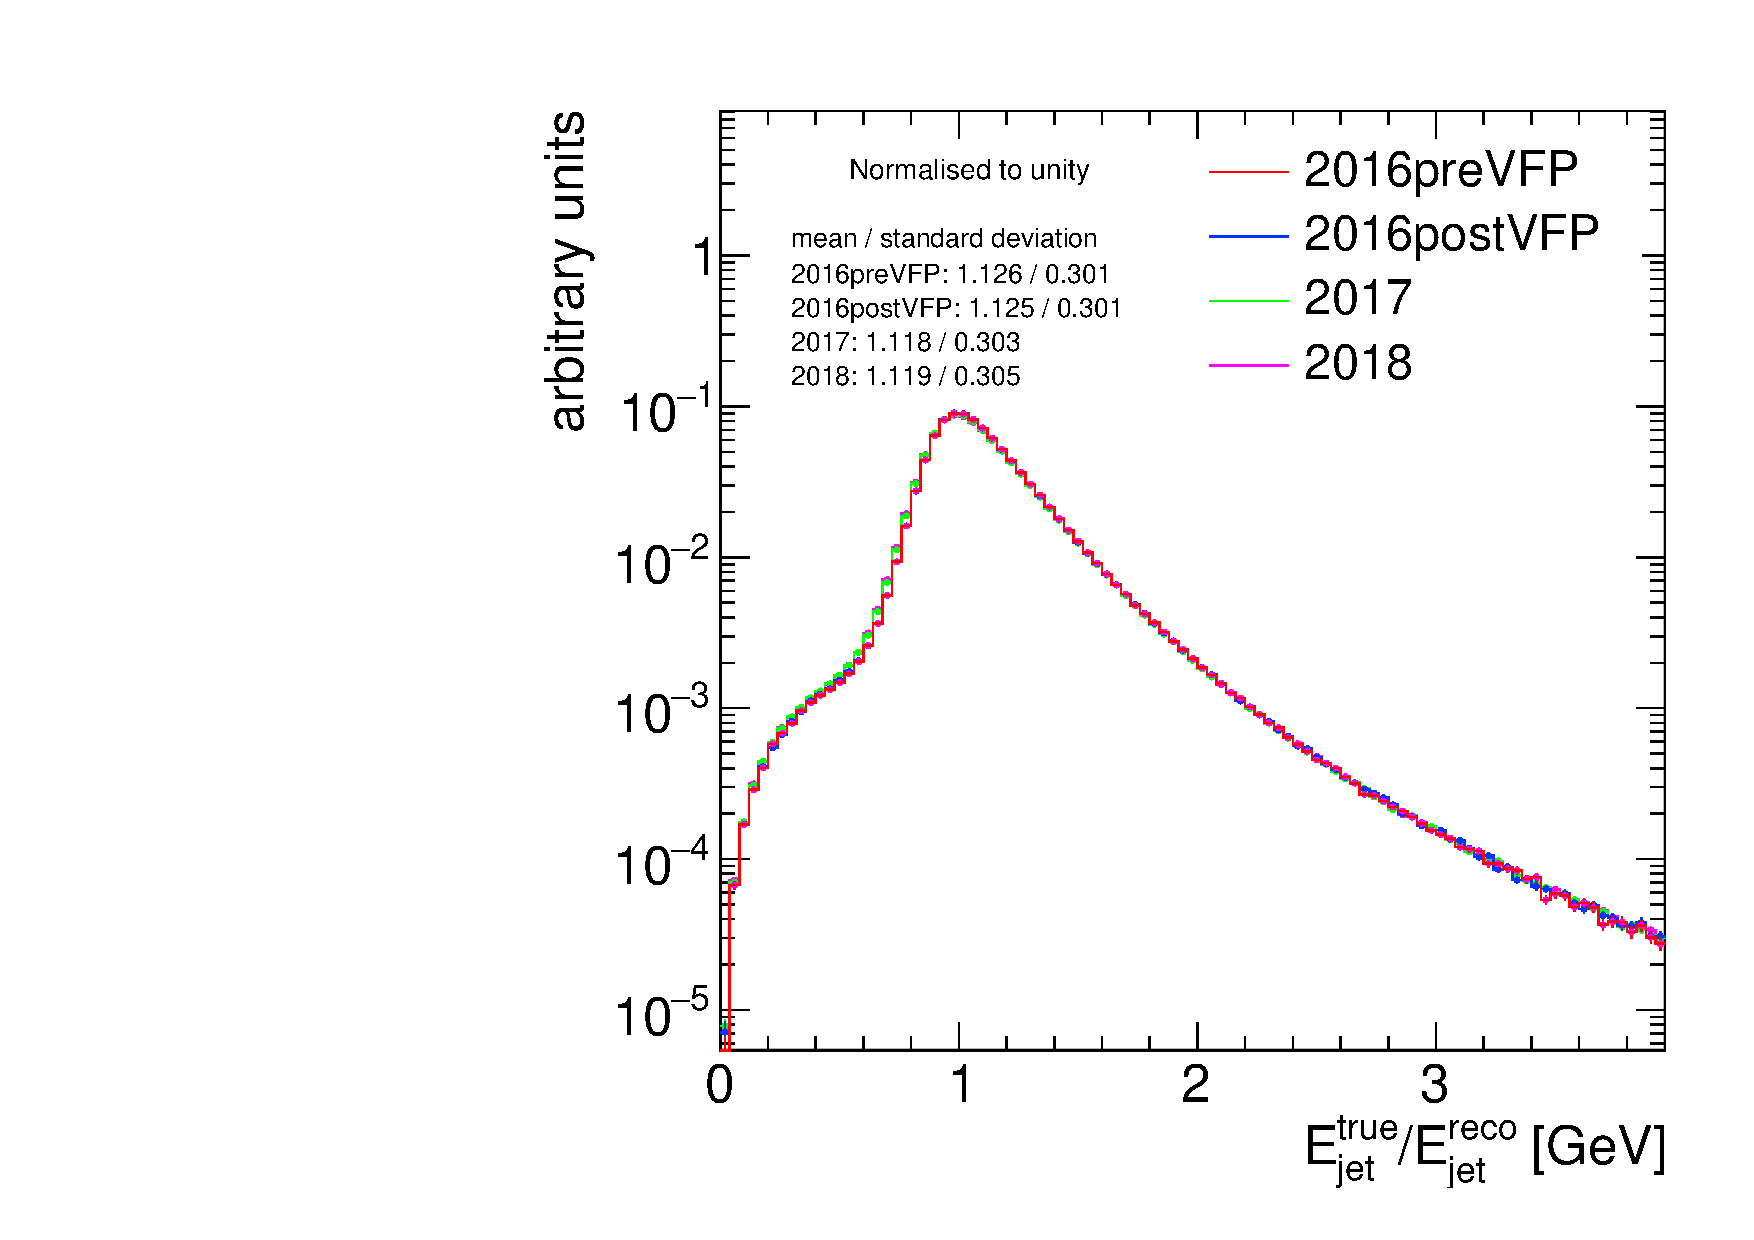
\includegraphics[width=0.30\textwidth]{fig_fullRun2UL/SmearingPlots/ULcomp_KinReco_fE_jet_step7.pdf}
        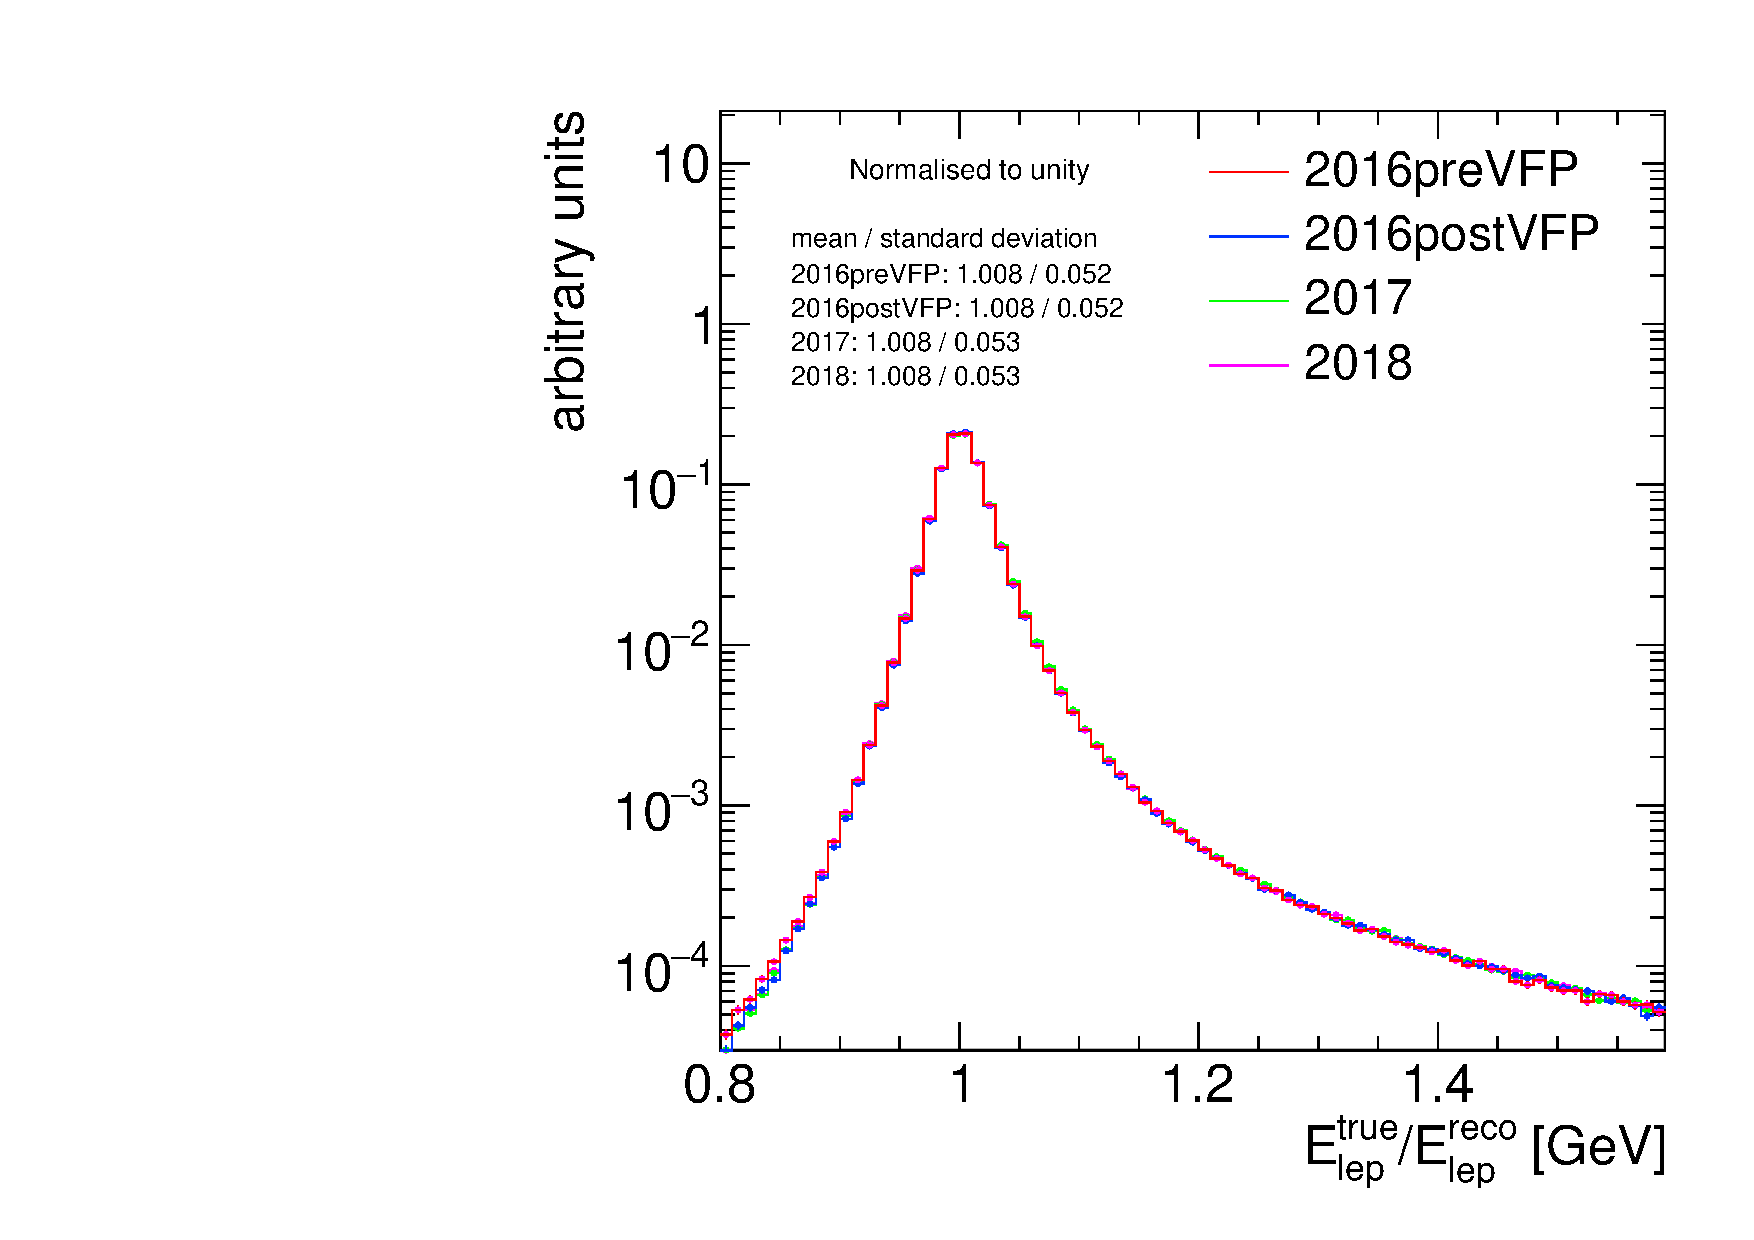
\includegraphics[width=0.30\textwidth]{fig_fullRun2UL/SmearingPlots/ULcomp_KinReco_fE_lep_step7.pdf}
        \caption{\small Distributions of the true energy divided by the reconstructed energy used for the energy smearing in the \ttbar full kinematic reconstruction. 
        The factors are shown for the b quarks (left) and the leptons (right).}
    \label{fig:energyFactor}
    \end{center}
\end{figure}

\begin{figure}[!htb]
    \begin{center}
        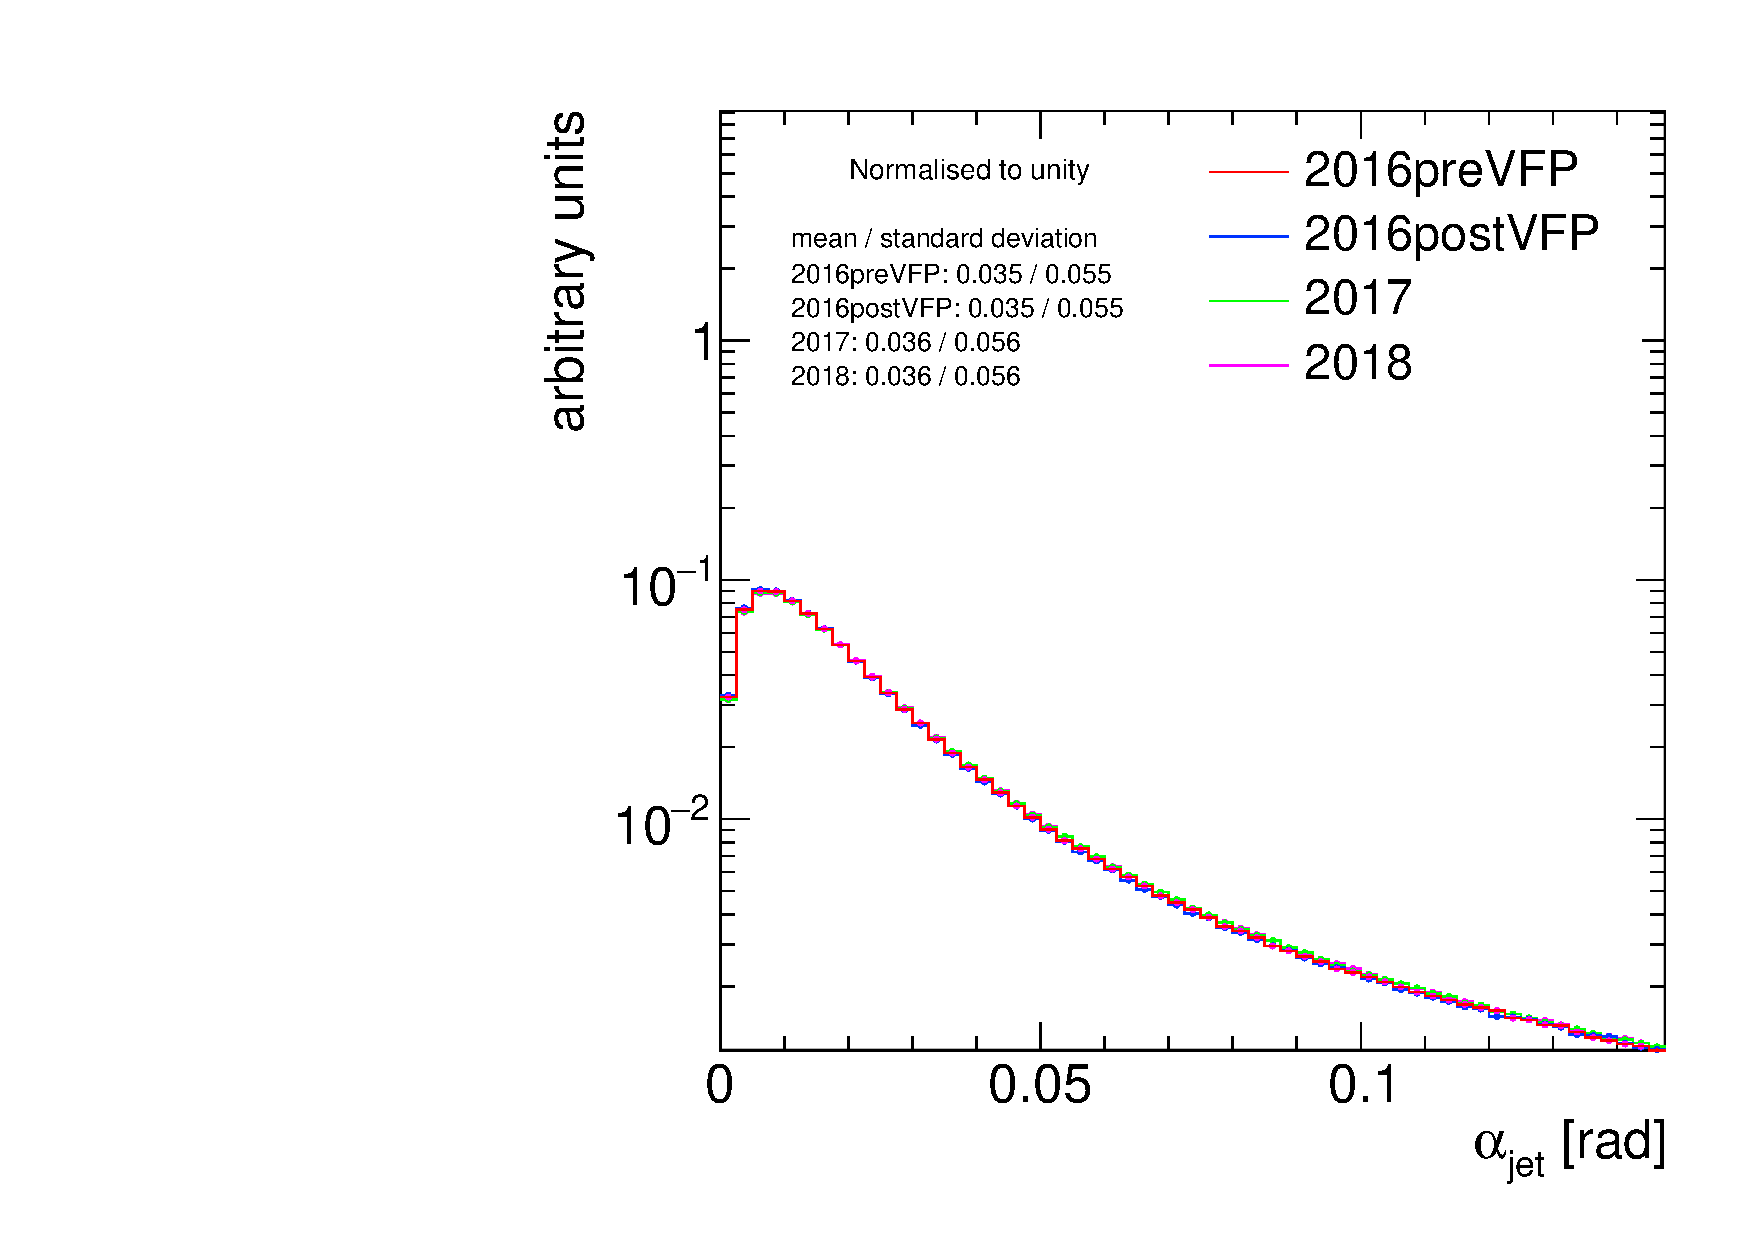
\includegraphics[width=0.30\textwidth]{fig_fullRun2UL/SmearingPlots/ULcomp_KinReco_d_angle_jet_step7.pdf}
        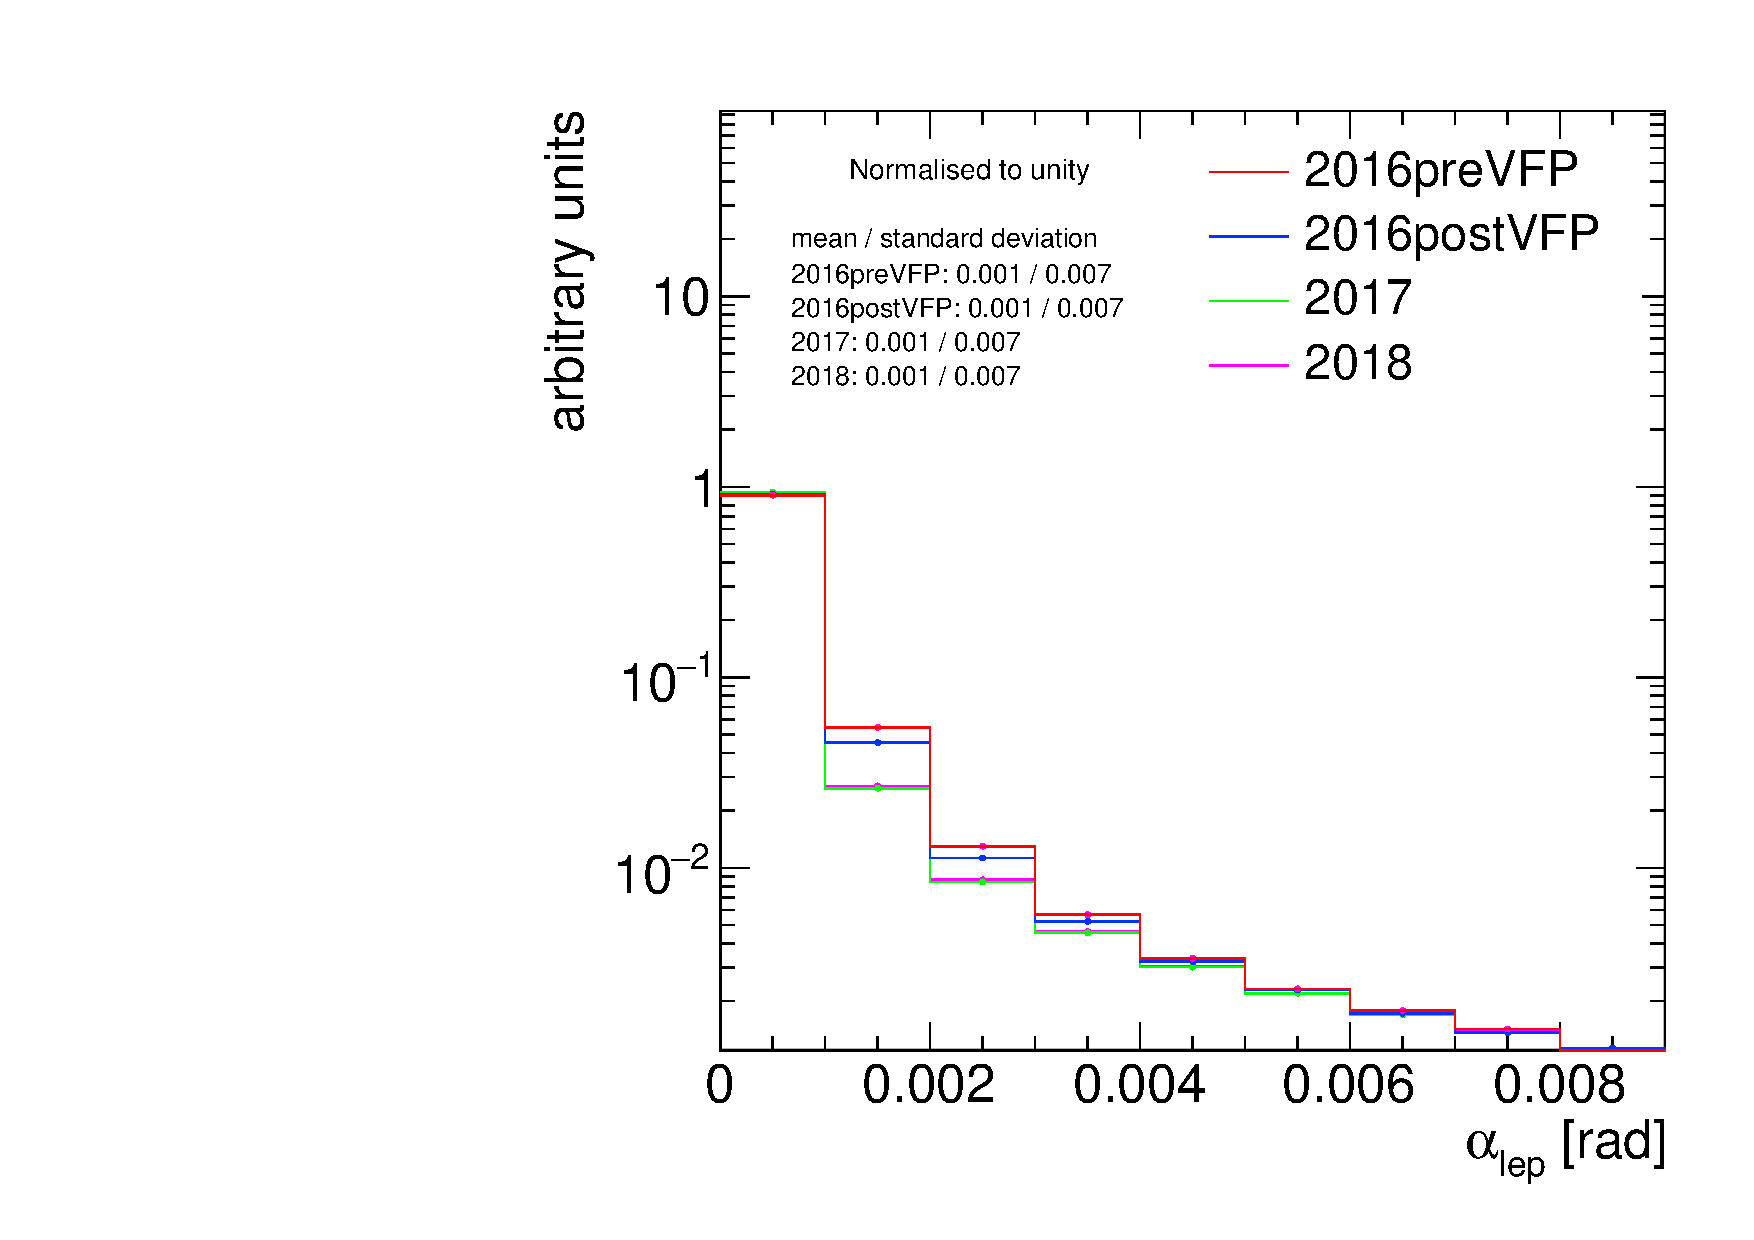
\includegraphics[width=0.30\textwidth]{fig_fullRun2UL/SmearingPlots/ULcomp_KinReco_d_angle_lep_step7.pdf}
        \caption{\small Distributions of the angle between the true direction and the reconstructed direction for jets (left) and leptons (right).}
       \label{fig:angleFactor}
    \end{center}
\end{figure}

\begin{figure}[!htb]
    \begin{center}
        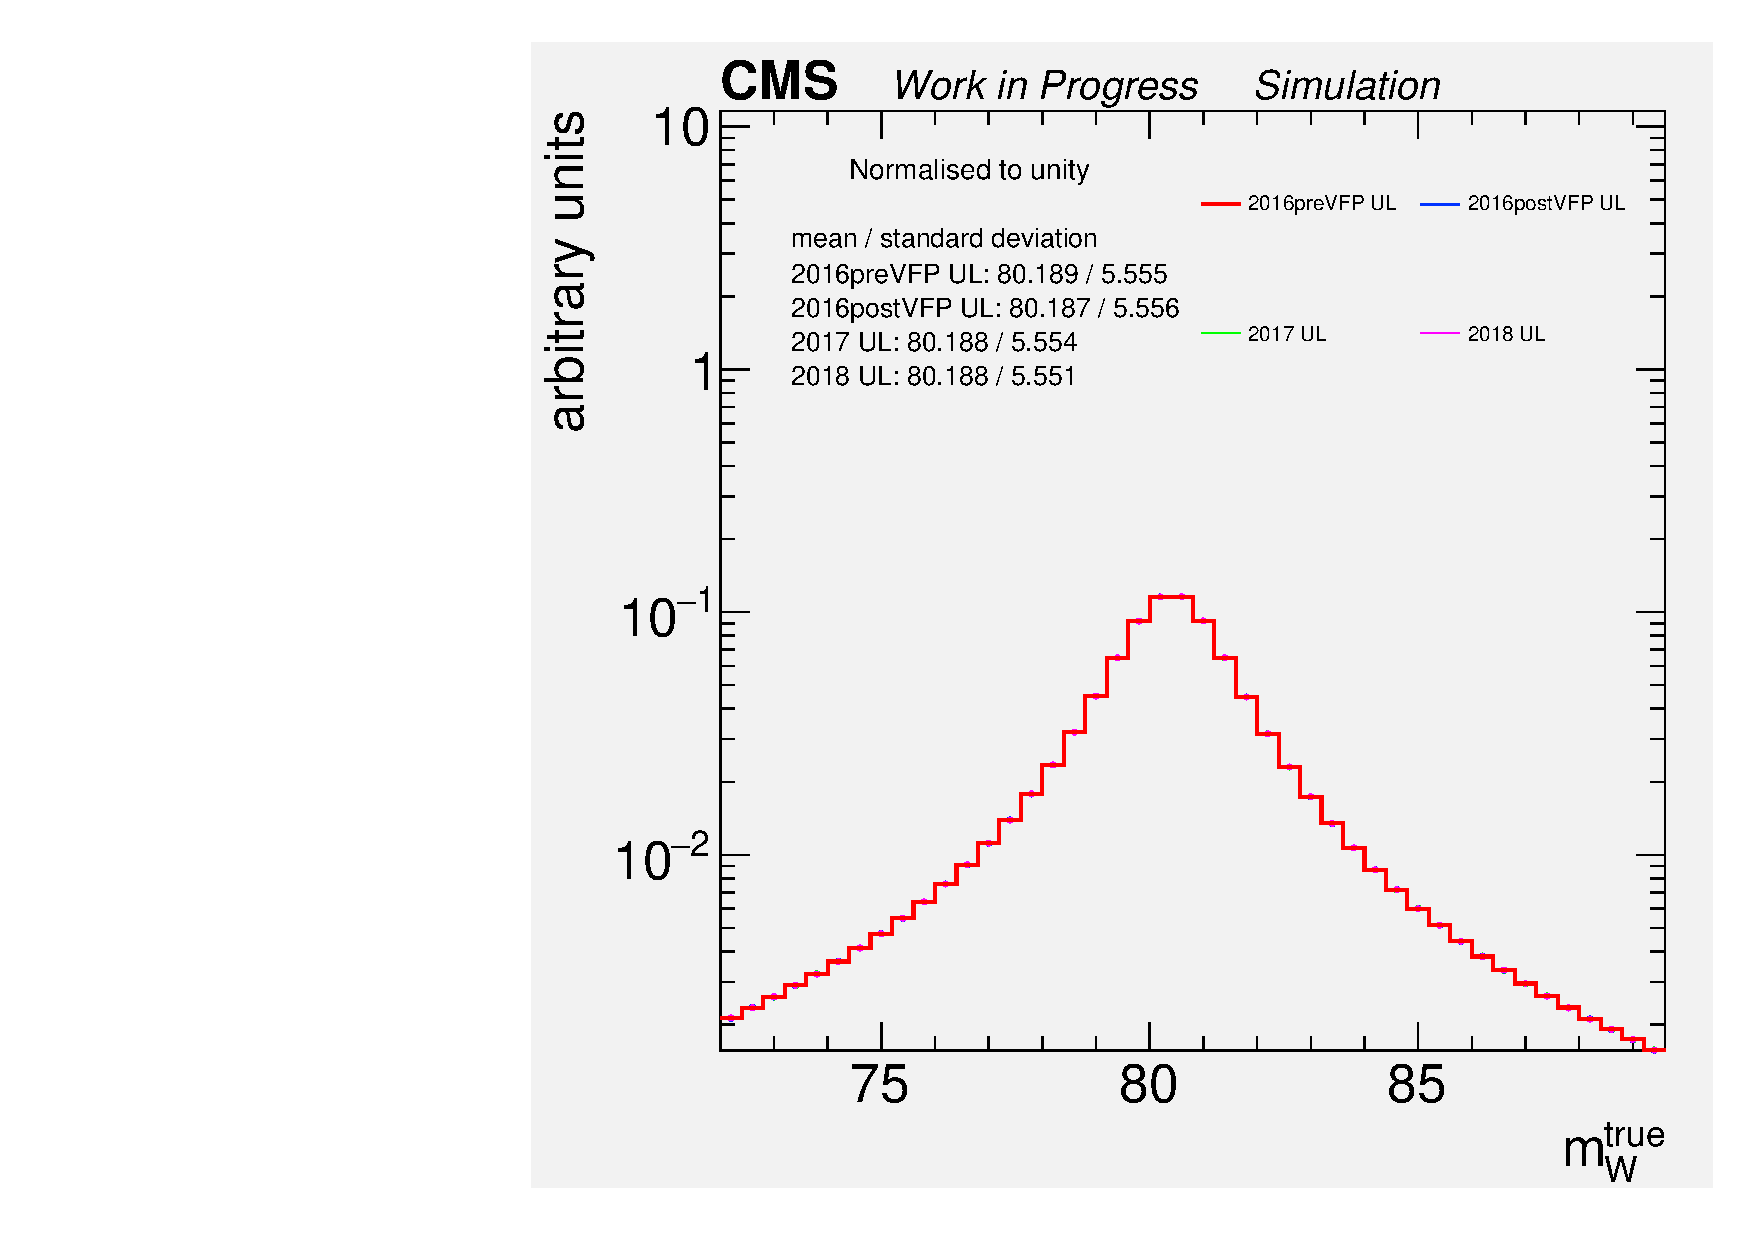
\includegraphics[width=0.30\textwidth]{fig_fullRun2UL/SmearingPlots/ULcomp_KinReco_W_mass_step0.pdf}
        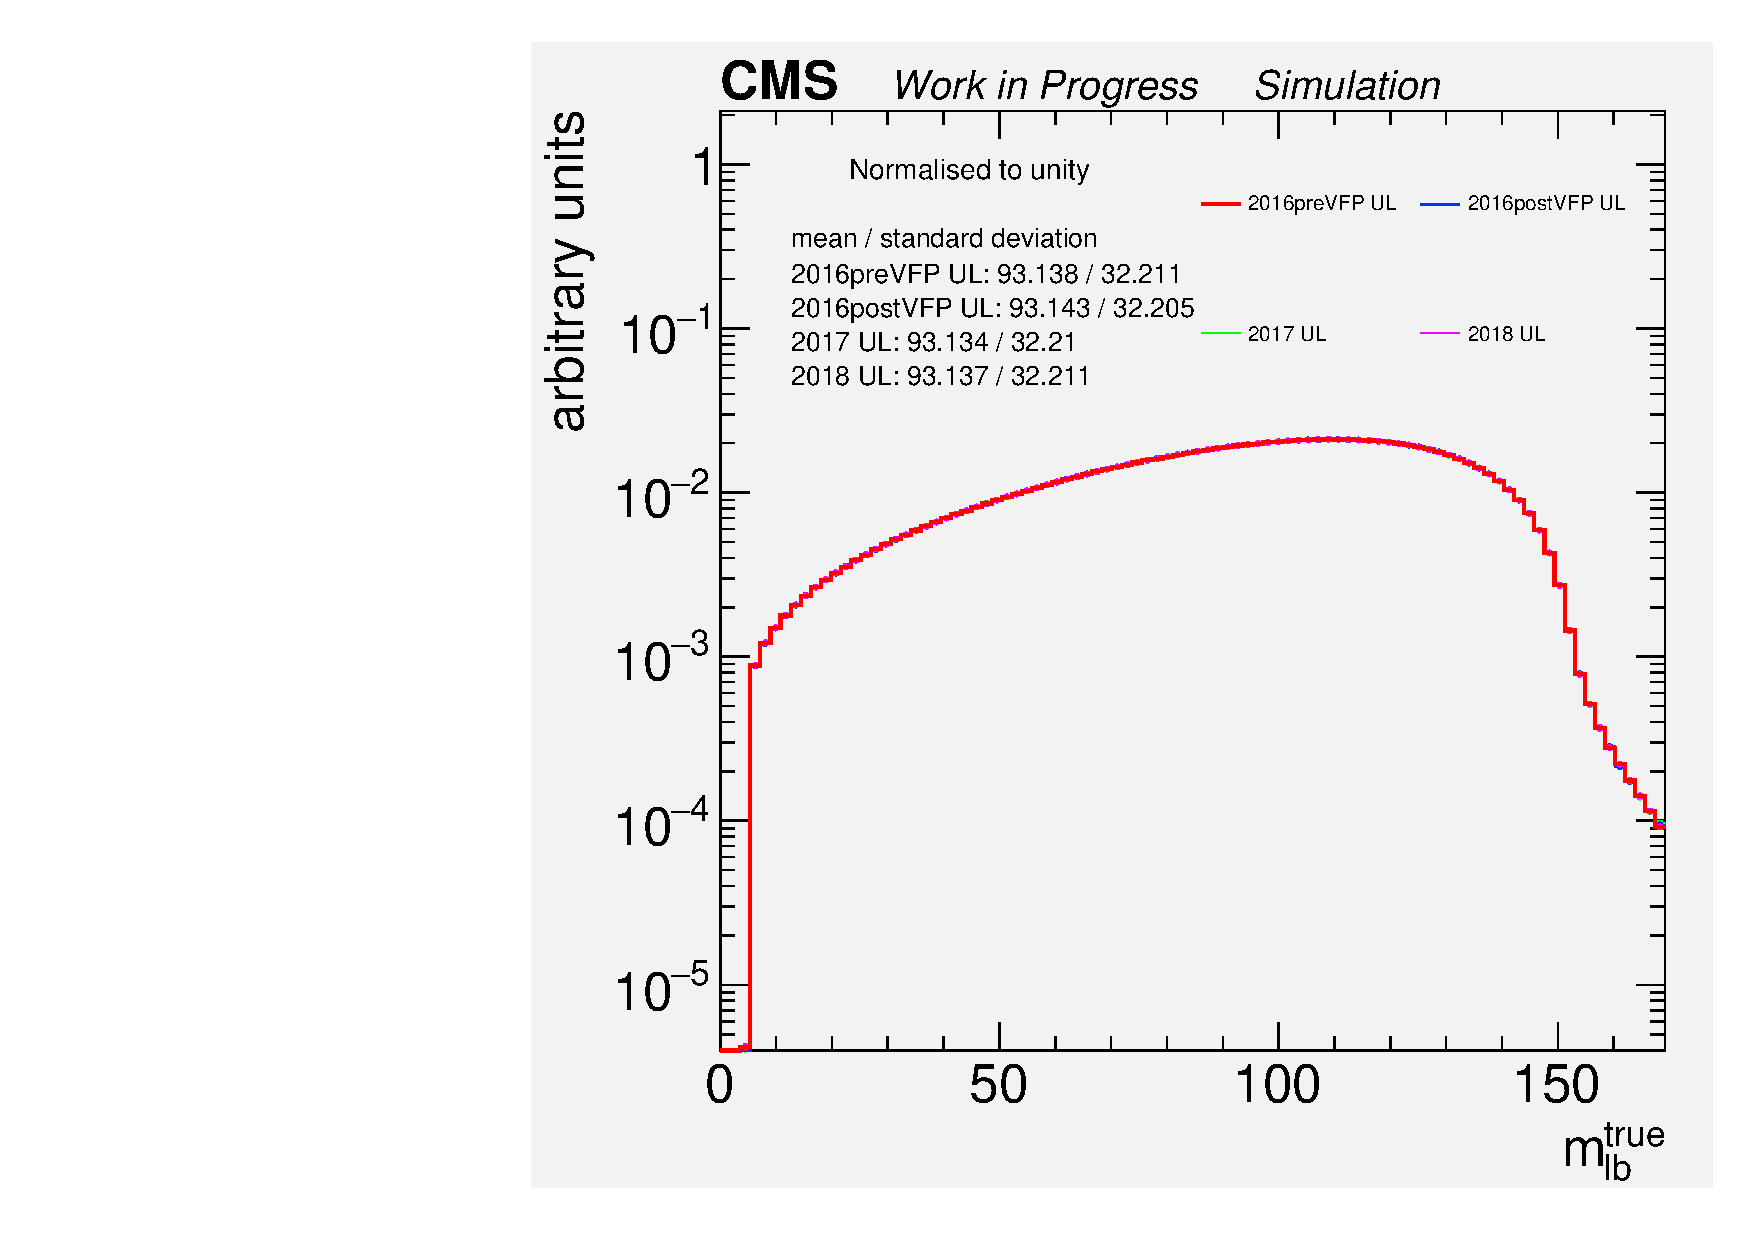
\includegraphics[width=0.30\textwidth]{fig_fullRun2UL/SmearingPlots/ULcomp_KinReco_mbl_true_step0.pdf}
        \caption{\small Distributions of the true W boson mass (left) and invariant mass distribution of reconstructed leptons and b-jets (right).}
       \label{fig:inputDists}
    \end{center}
\end{figure}

Likelihood weights for each smeared solution are calculated from the invariant mass of reconstructed leptons and b-jets relative to the true invariant mass distributions.
The true lepton-b-jet invariant mass distribution used to calculated solution likelihood weights is shown in figure~\ref{fig:inputDists}.
For each smearing, the jet--lepton assignments which yield the maximum weight are chosen.
A weighted average of all smeared solutions provides the final solution to the top quark three-momentum:
\begin{align}
\langle \vec{p}_{t} \rangle = \frac{1}{\mathcal{W}_s} \sum_{i=1}^{100} \mathcal{W}_i \cdot \vec{p}_{t,\,i} \quad \mbox{with} \quad \mathcal{W}_s = \sum_{i=1}^{100} \mathcal{W}_{i}
\end{align}
where $\mathcal{W}_i$ and $\vec{p}_{t,\,i}$ denote the weight and reconstructed top quark three-momentum obtained for the $i$-th smearing of the event.
Smearings without any solutions are given null weights.
The top quark energy is calculated from its three-momentum and the top quark mass constraint $m_{t} = \SI{172.5}{\GeV}$.
The final solution for top anti-quark four-momentum determined in an analogous procedure.

\subsection{Comparison of \ensuremath{\mathrm{t\bar{t}}} Reconstruction for Prompt and Via \ensuremath{\mathrm{\tau}} Dilepton Events}
The assumption that the dilepton decay is prompt and there are only two neutrinos in the final state is not true when the dilepton decay is via intermediate $\tau$ leptons; such decays can have four or six neutrinos in the final state.
The top quark and \ttbar reconstructed kinematic variables at detector level (REC) are presented versus the true variables at generator level (GEN), and additionally the resolutions are presented as the difference between the true and reconstructed variables in bins of the true variables. 
Figures~\ref{fig:kinrec:resolution-mtt} through~\ref{fig:kinrec:resolution-yt} show resolution of \mtt, \ytt, \pttt, \yt, and \ptt\ distributions for both prompt and via tau reconstructed \ttbar dilepton events. 
The mean and sigma from a Gaussian fit to the kinematic variable resolutions are also included and reflect the bias and resolution of the algorithm, including degradation attributed to wrong jet--lepton assignments. 
We conclude that the resolution of \ttbar dilepton events via $\tau$ are comparable to prompt events, and thus are included as signal in this measurement.

\begin{figure}
  \begin{center}
    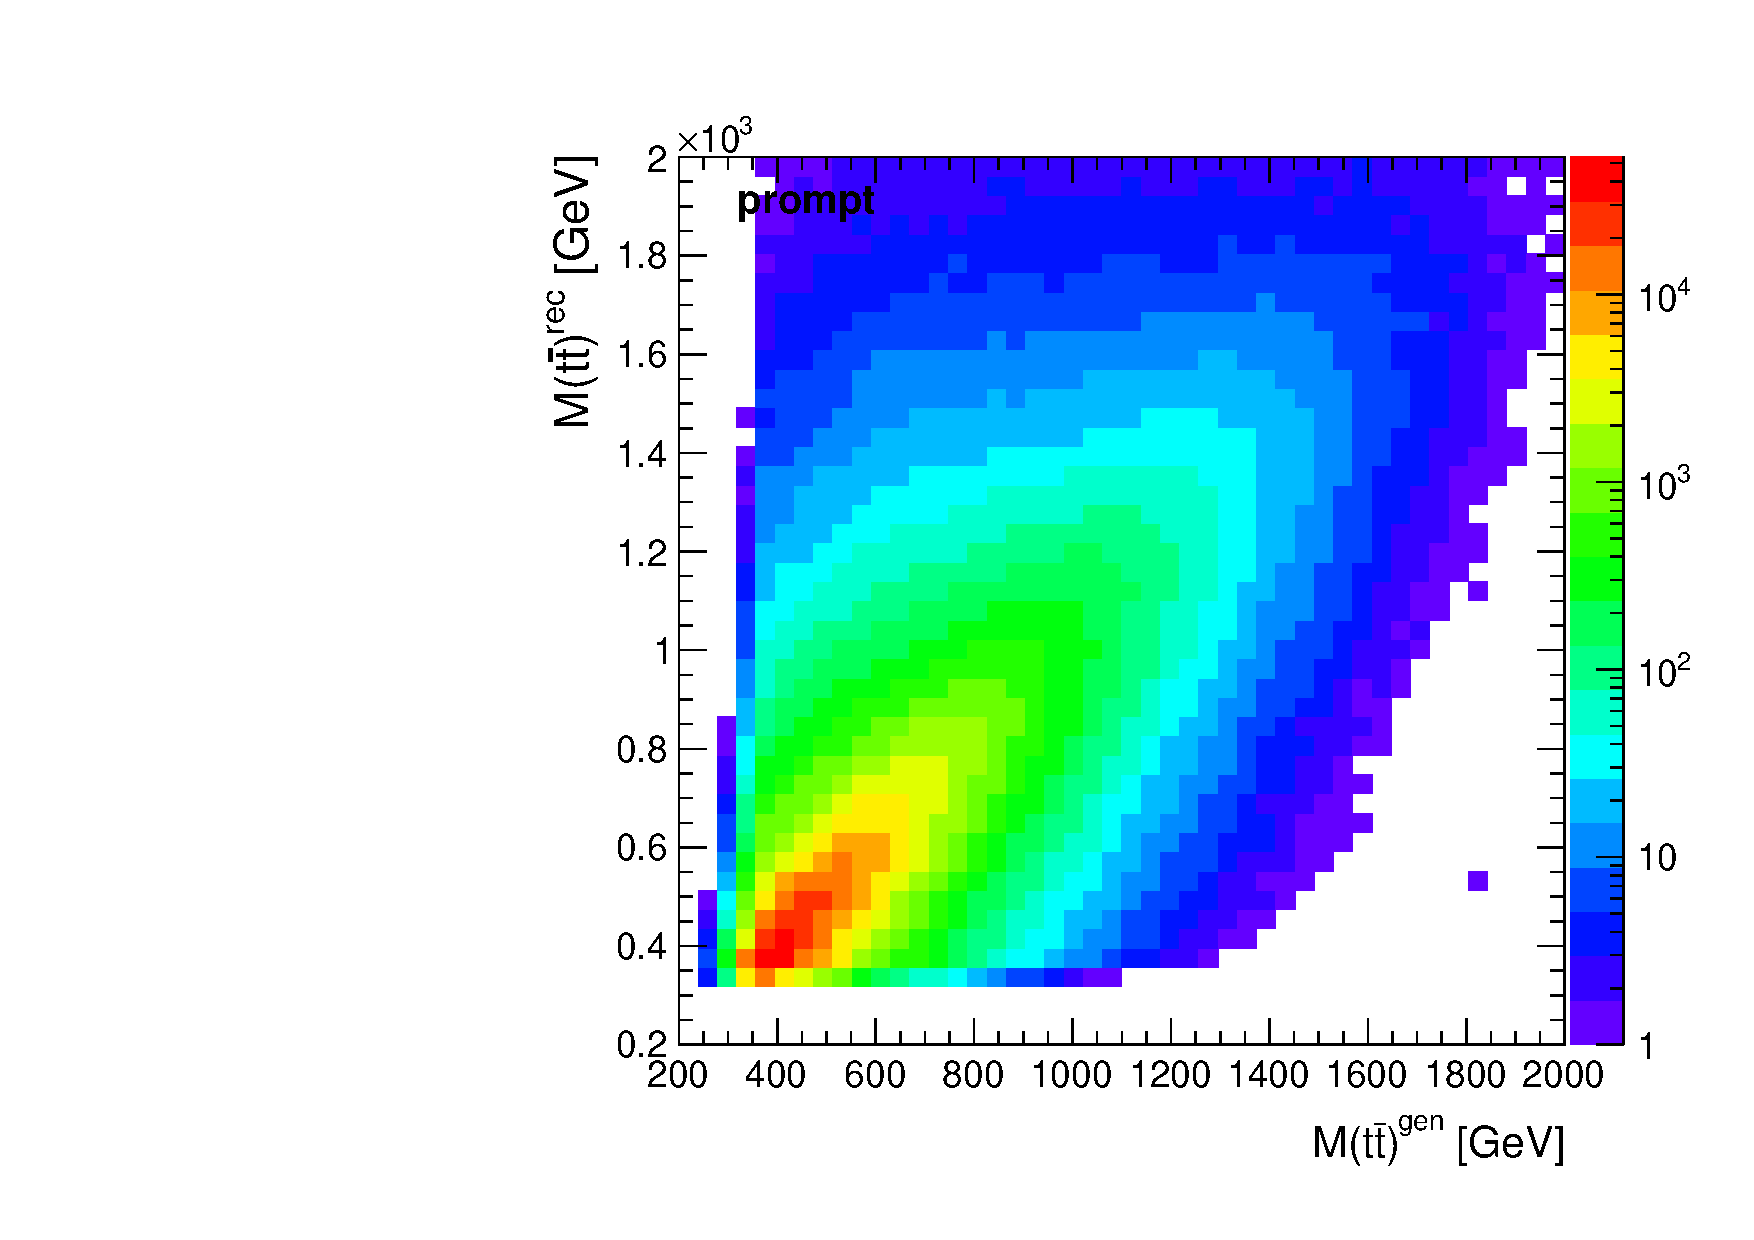
\includegraphics[width=0.30\textwidth]{fig_fullRun2UL/KinRecoResolutions/ttbar_mass_genreco_prompt.pdf}
    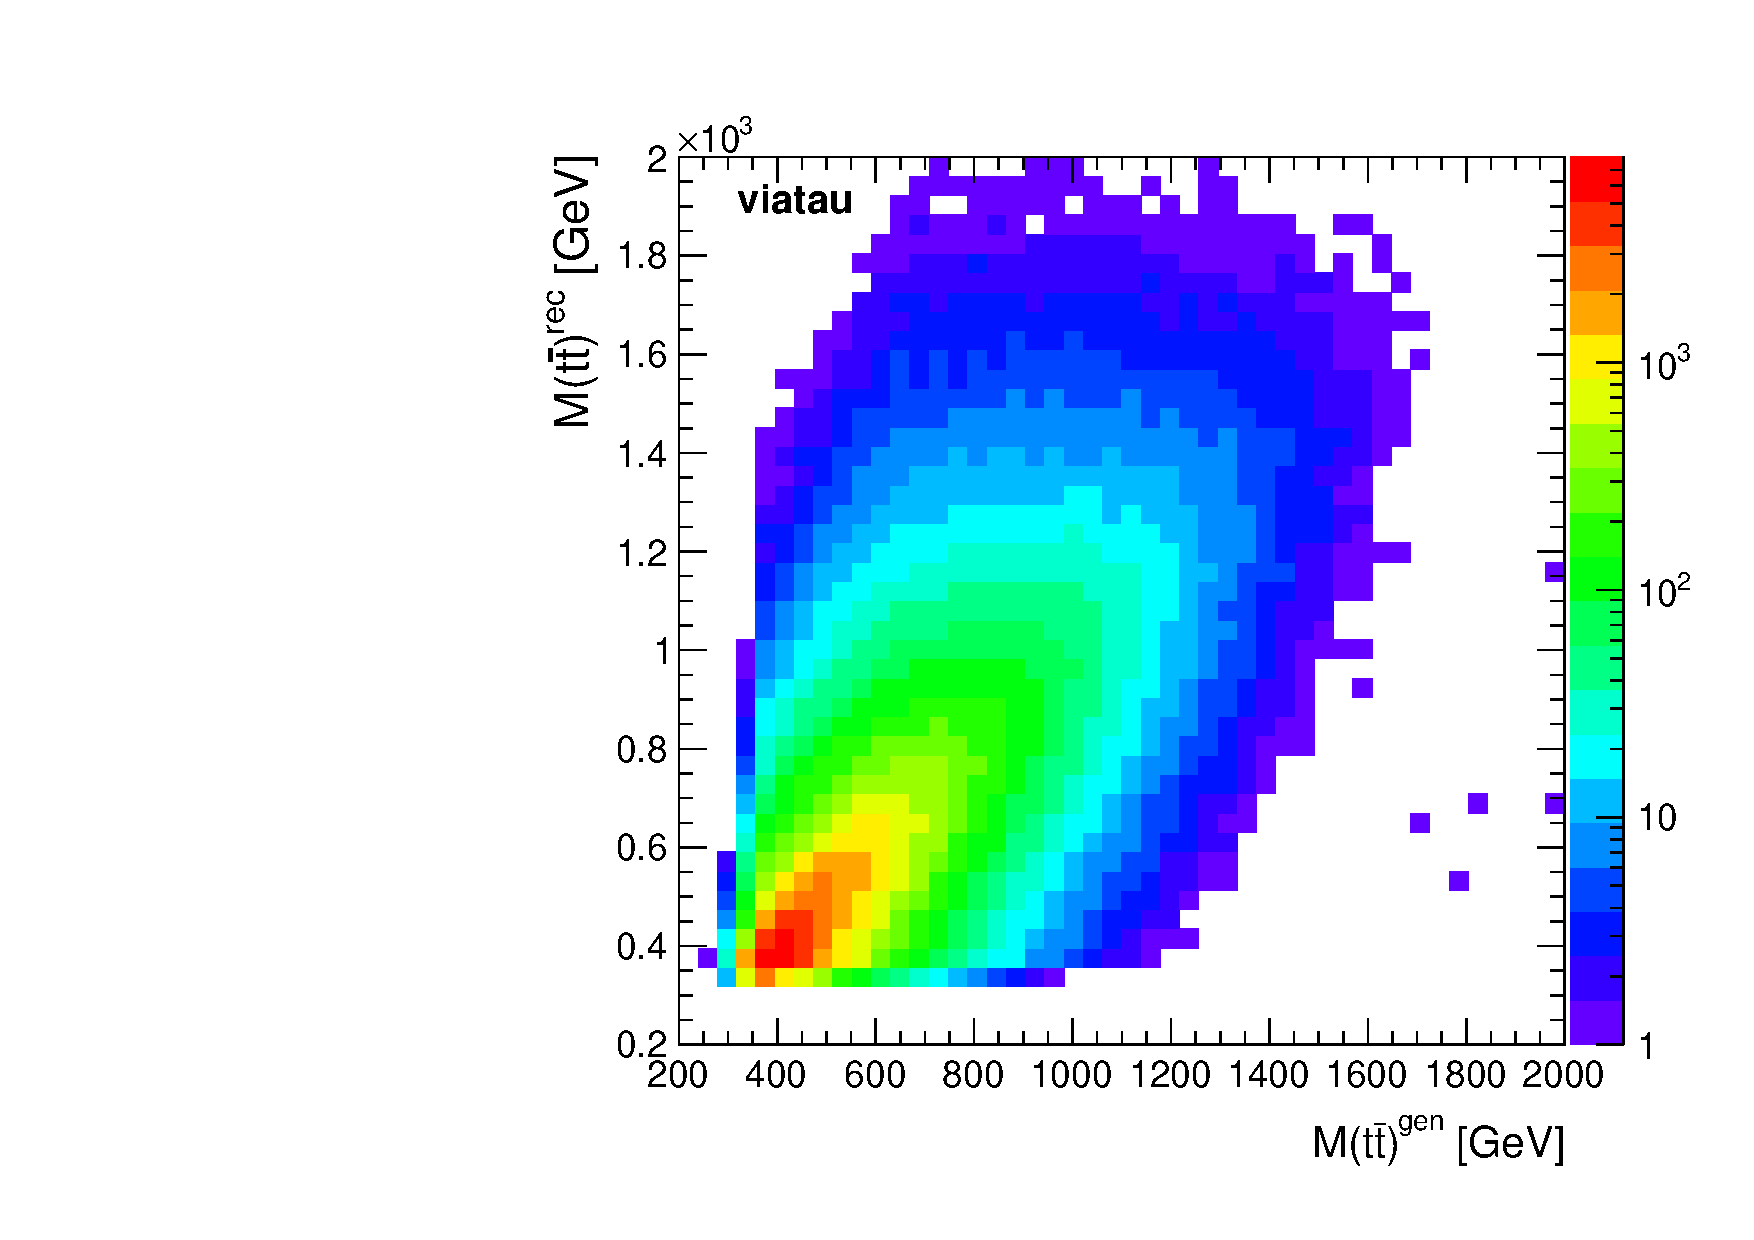
\includegraphics[width=0.30\textwidth]{fig_fullRun2UL/KinRecoResolutions/ttbar_mass_genreco_viatau.pdf}\\
    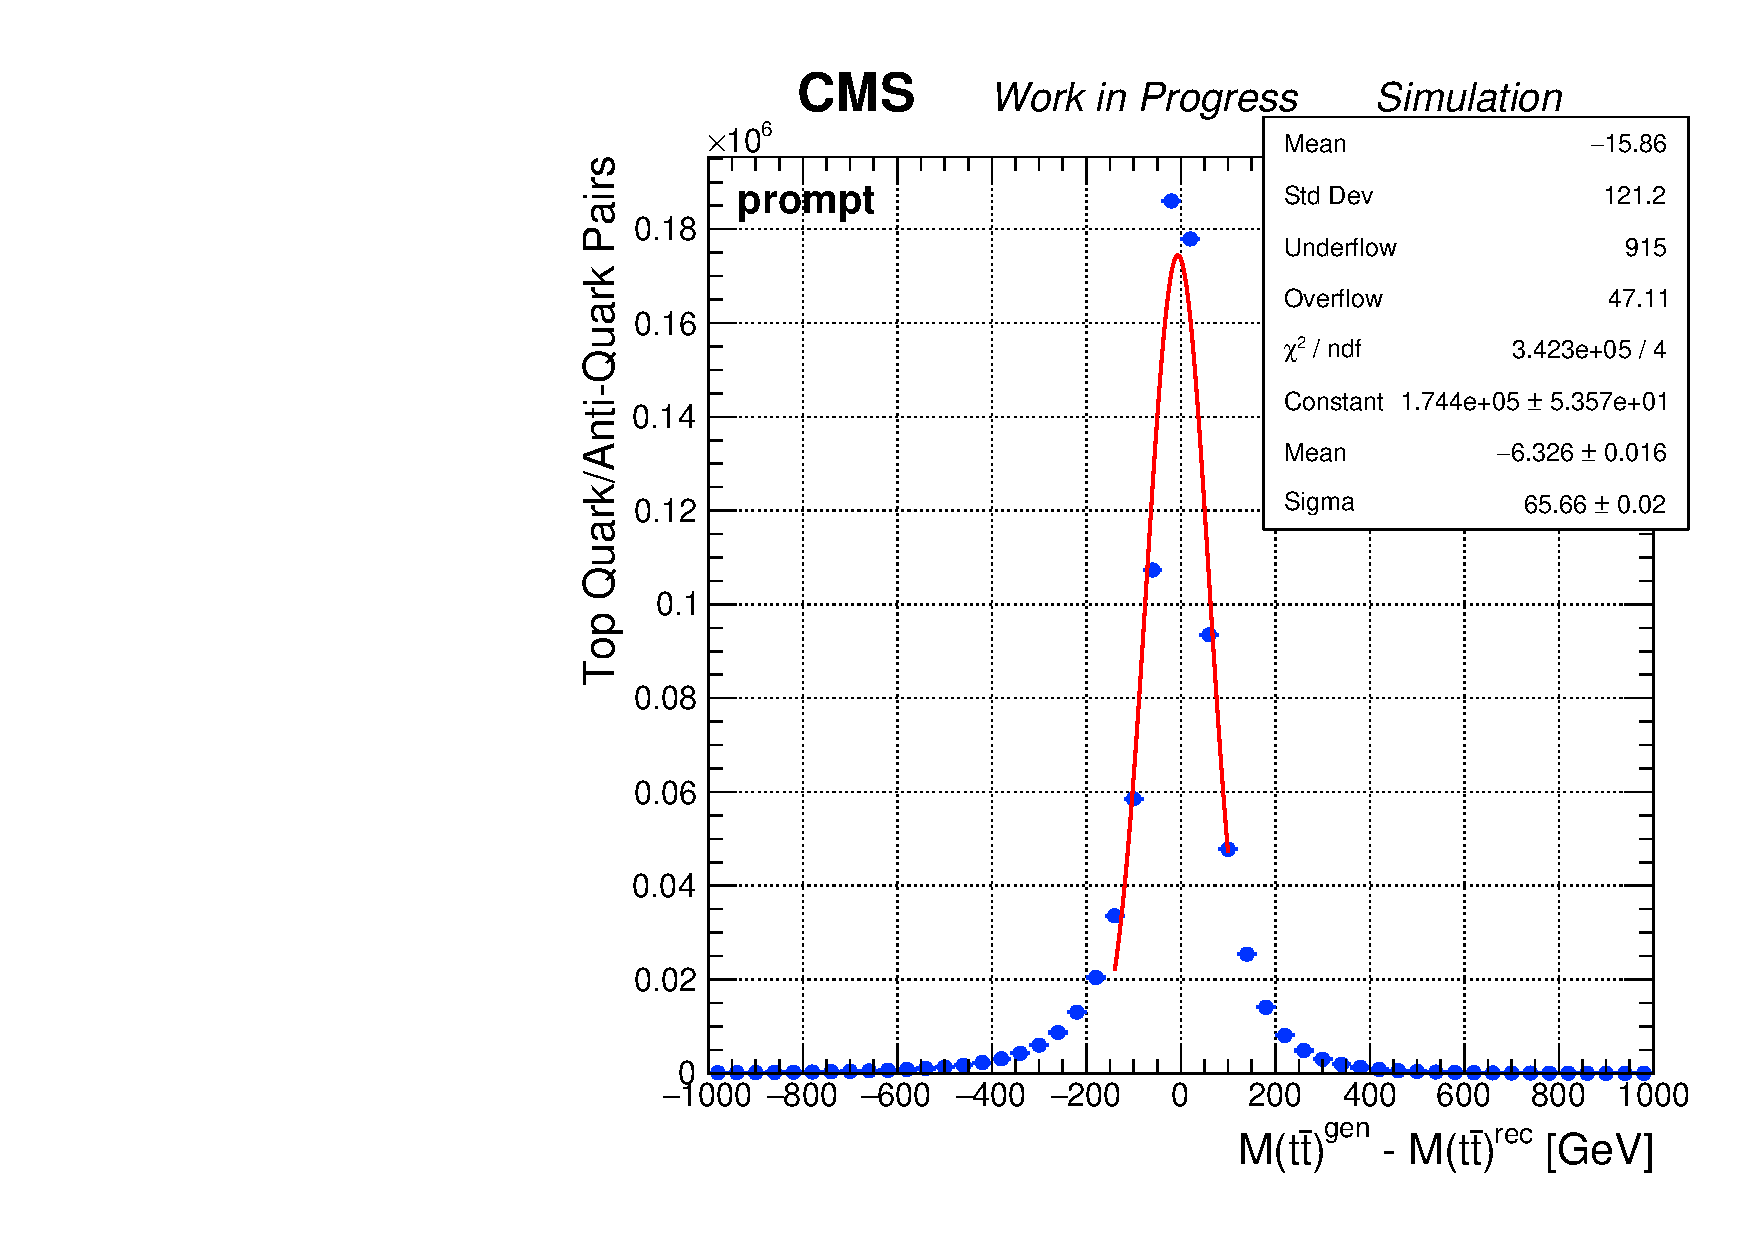
\includegraphics[width=0.30\textwidth]{fig_fullRun2UL/KinRecoResolutions/ttbar_mass_residual_prompt.pdf}
    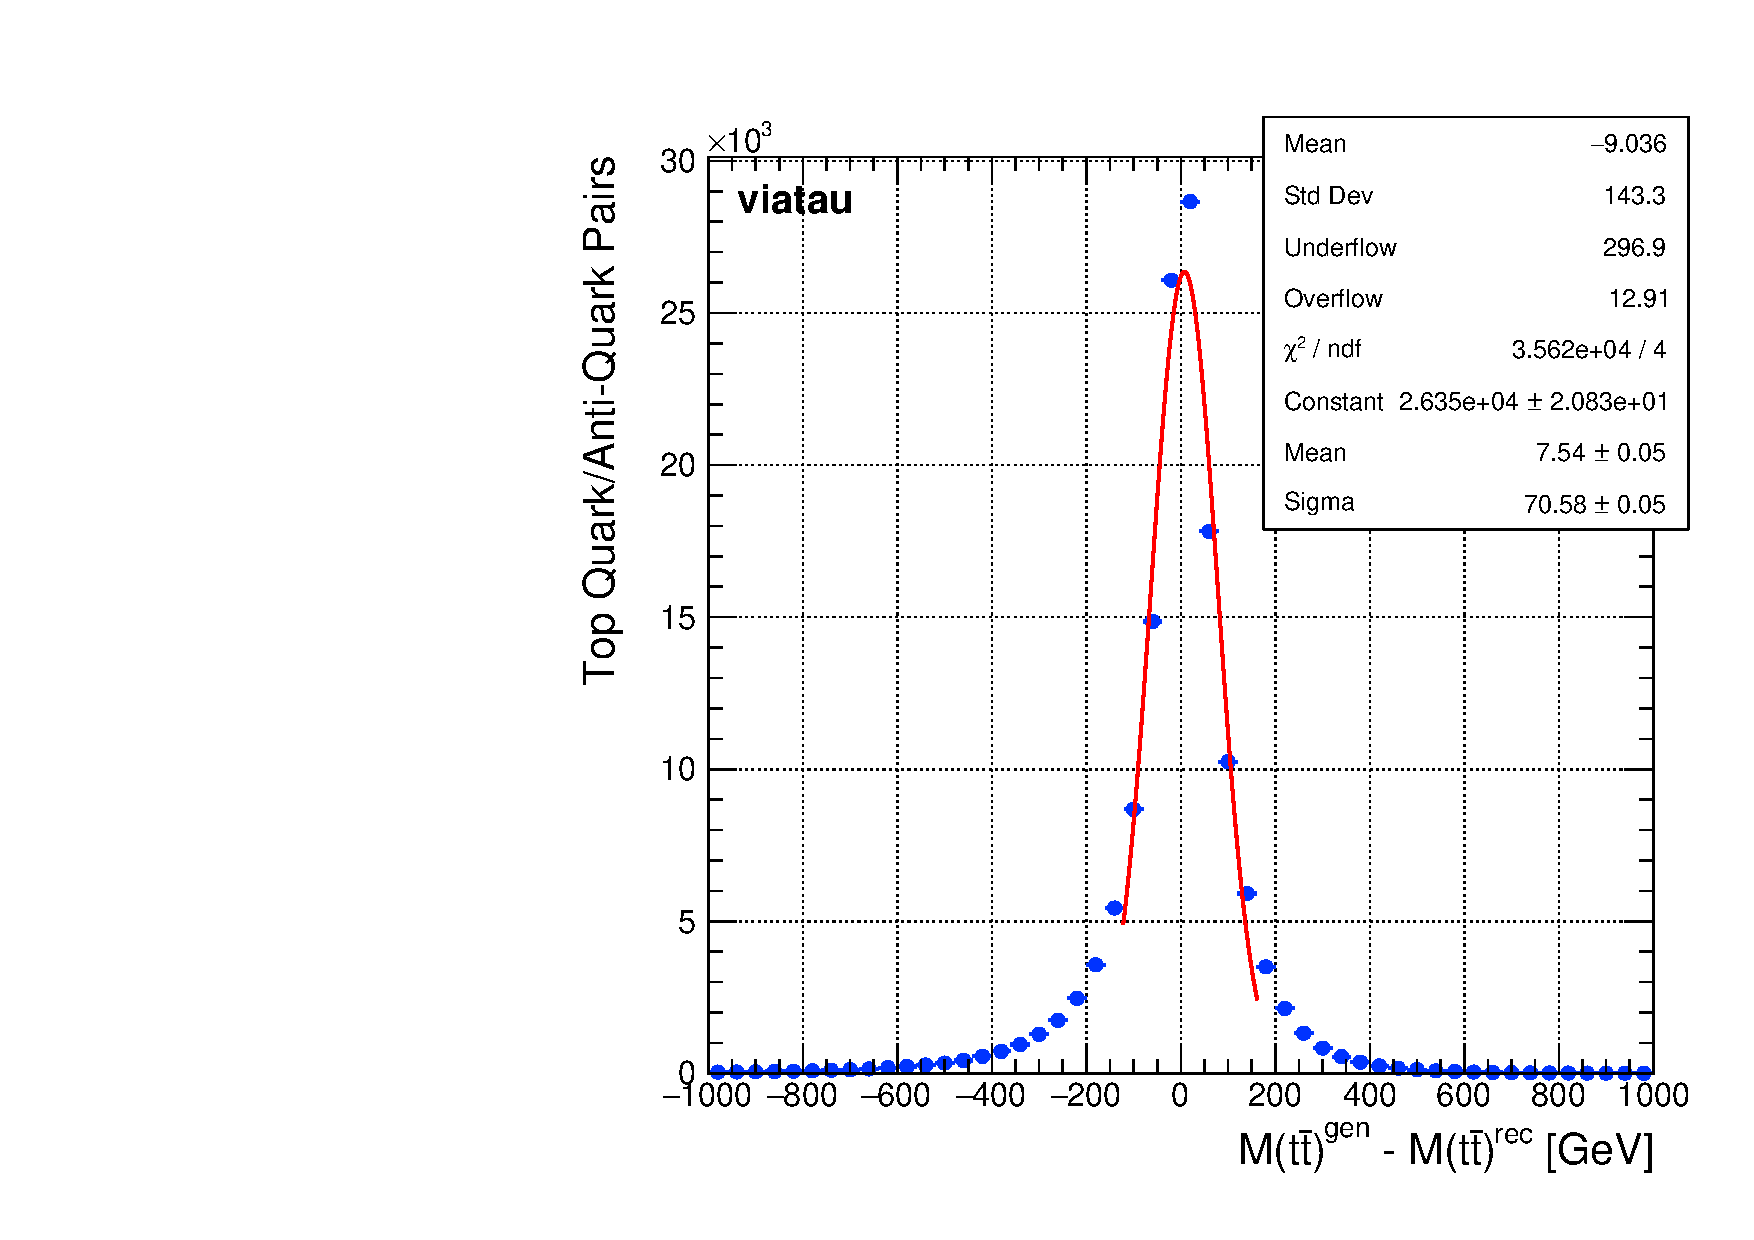
\includegraphics[width=0.30\textwidth]{fig_fullRun2UL/KinRecoResolutions/ttbar_mass_residual_viatau.pdf}\\
    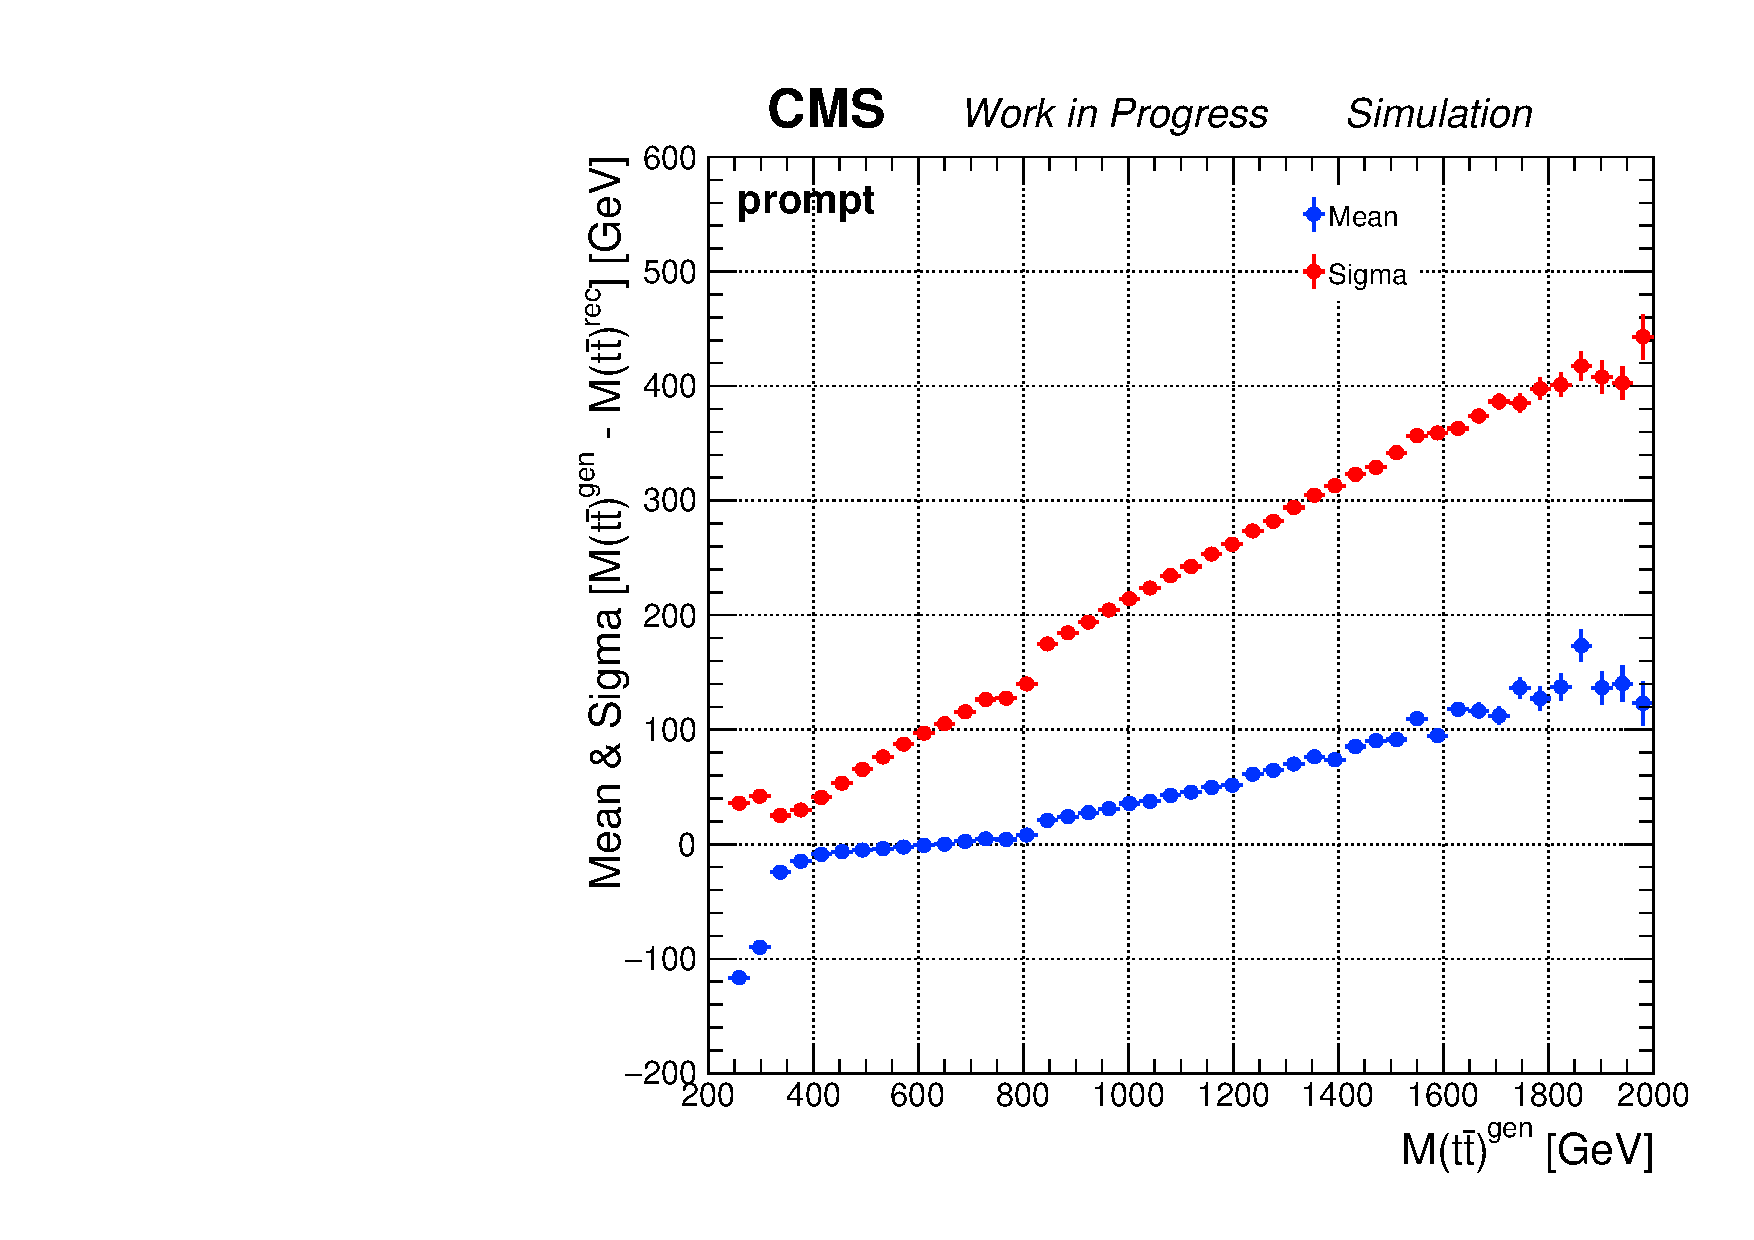
\includegraphics[width=0.30\textwidth]{fig_fullRun2UL/KinRecoResolutions/ttbar_mass_multiresidual_prompt.pdf}
    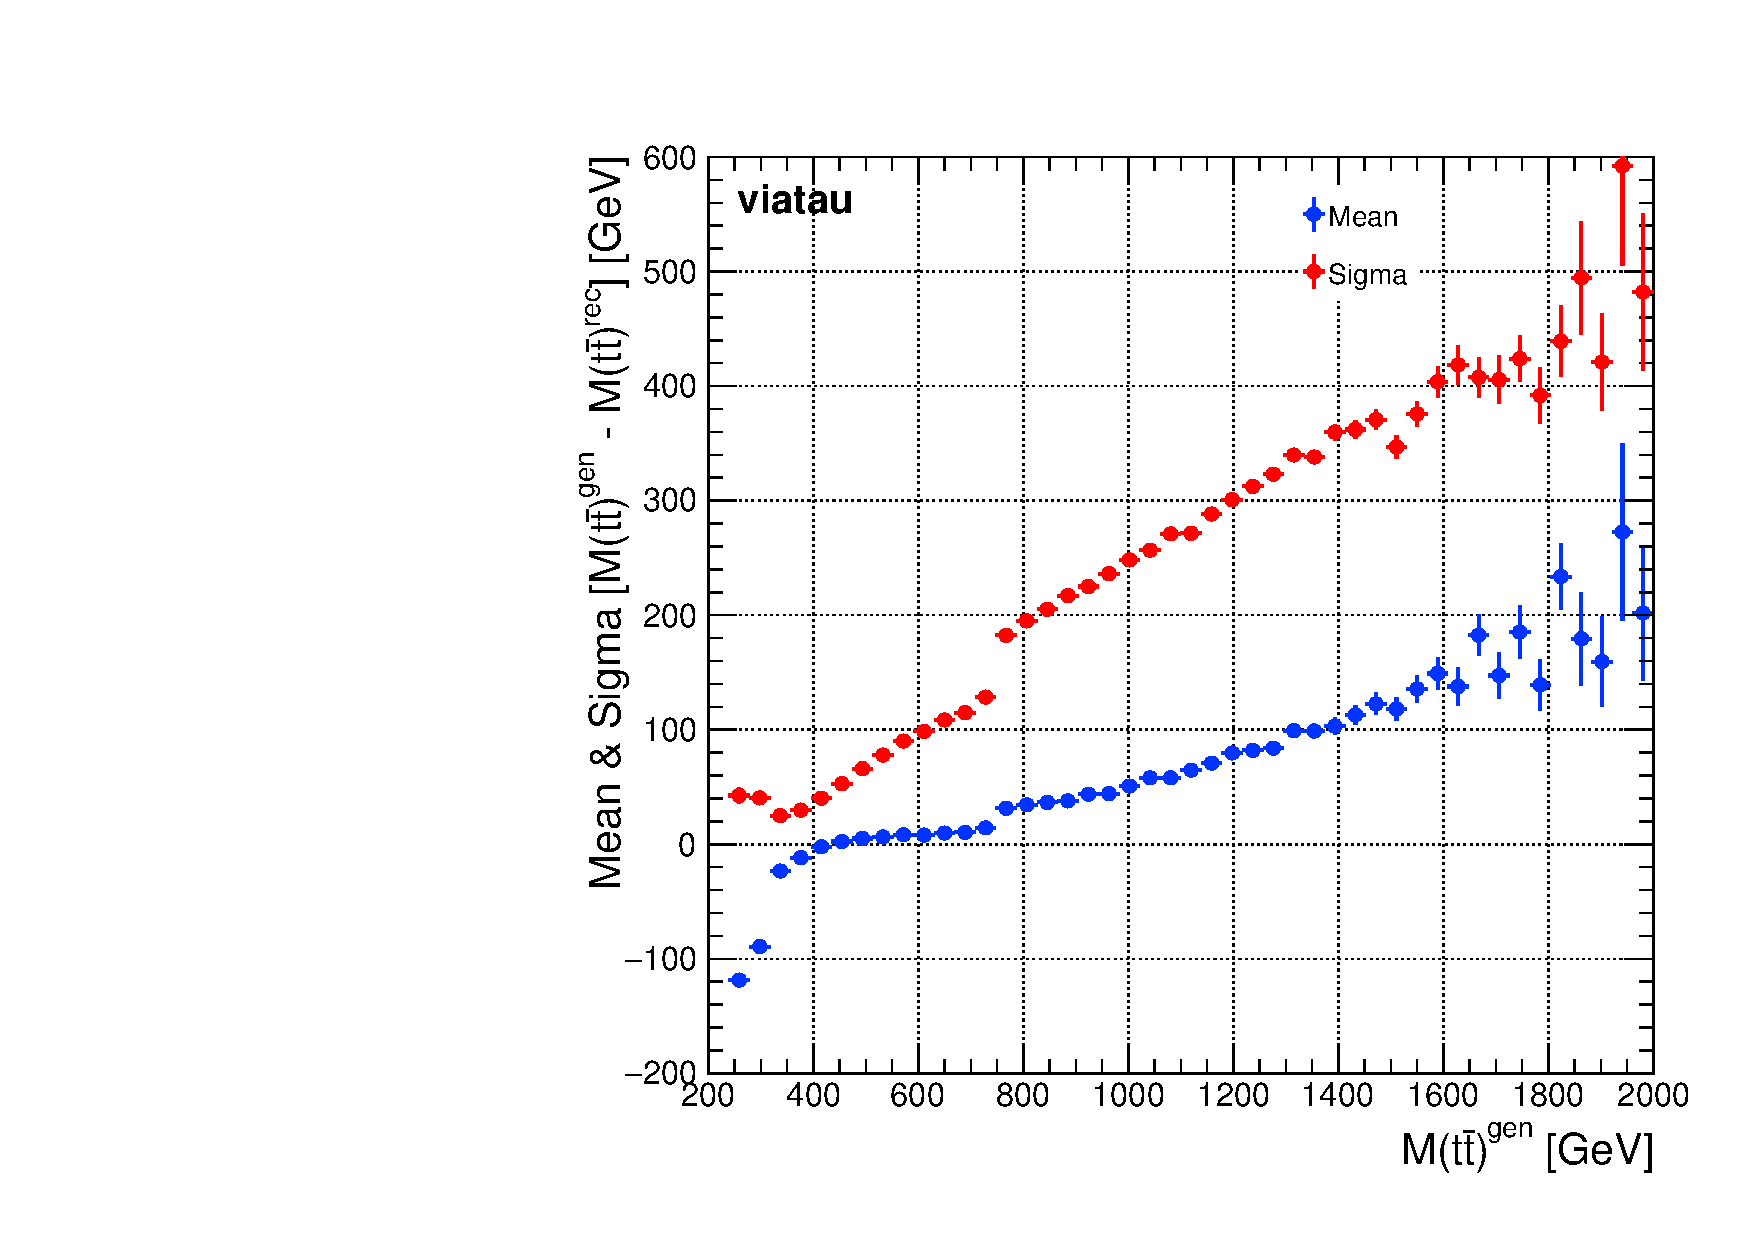
\includegraphics[width=0.30\textwidth]{fig_fullRun2UL/KinRecoResolutions/ttbar_mass_multiresidual_viatau.pdf}\\
    \caption{\small Top: True and reconstructed \mtt\ obtained for prompt (left) and via tau (right) \ttbar dilepton events.
    Middle: The difference between true and reconstructed \mtt\ in bins of true \mtt\ (fitted with a Gaussian function for illustration).
    Bottom: The differential mean and sigma from Gaussian fits, with respect to true \mtt, of the difference between true and reconstructed \mtt\ obtained for prompt and via tau \ttbar dilepton events.
    The simulated samples are normalized to an integrated luminosity of \lumivalueRuniiUL.}
    \label{fig:kinrec:resolution-mtt}
 \end{center}
\end{figure}

\begin{figure}
  \begin{center}
    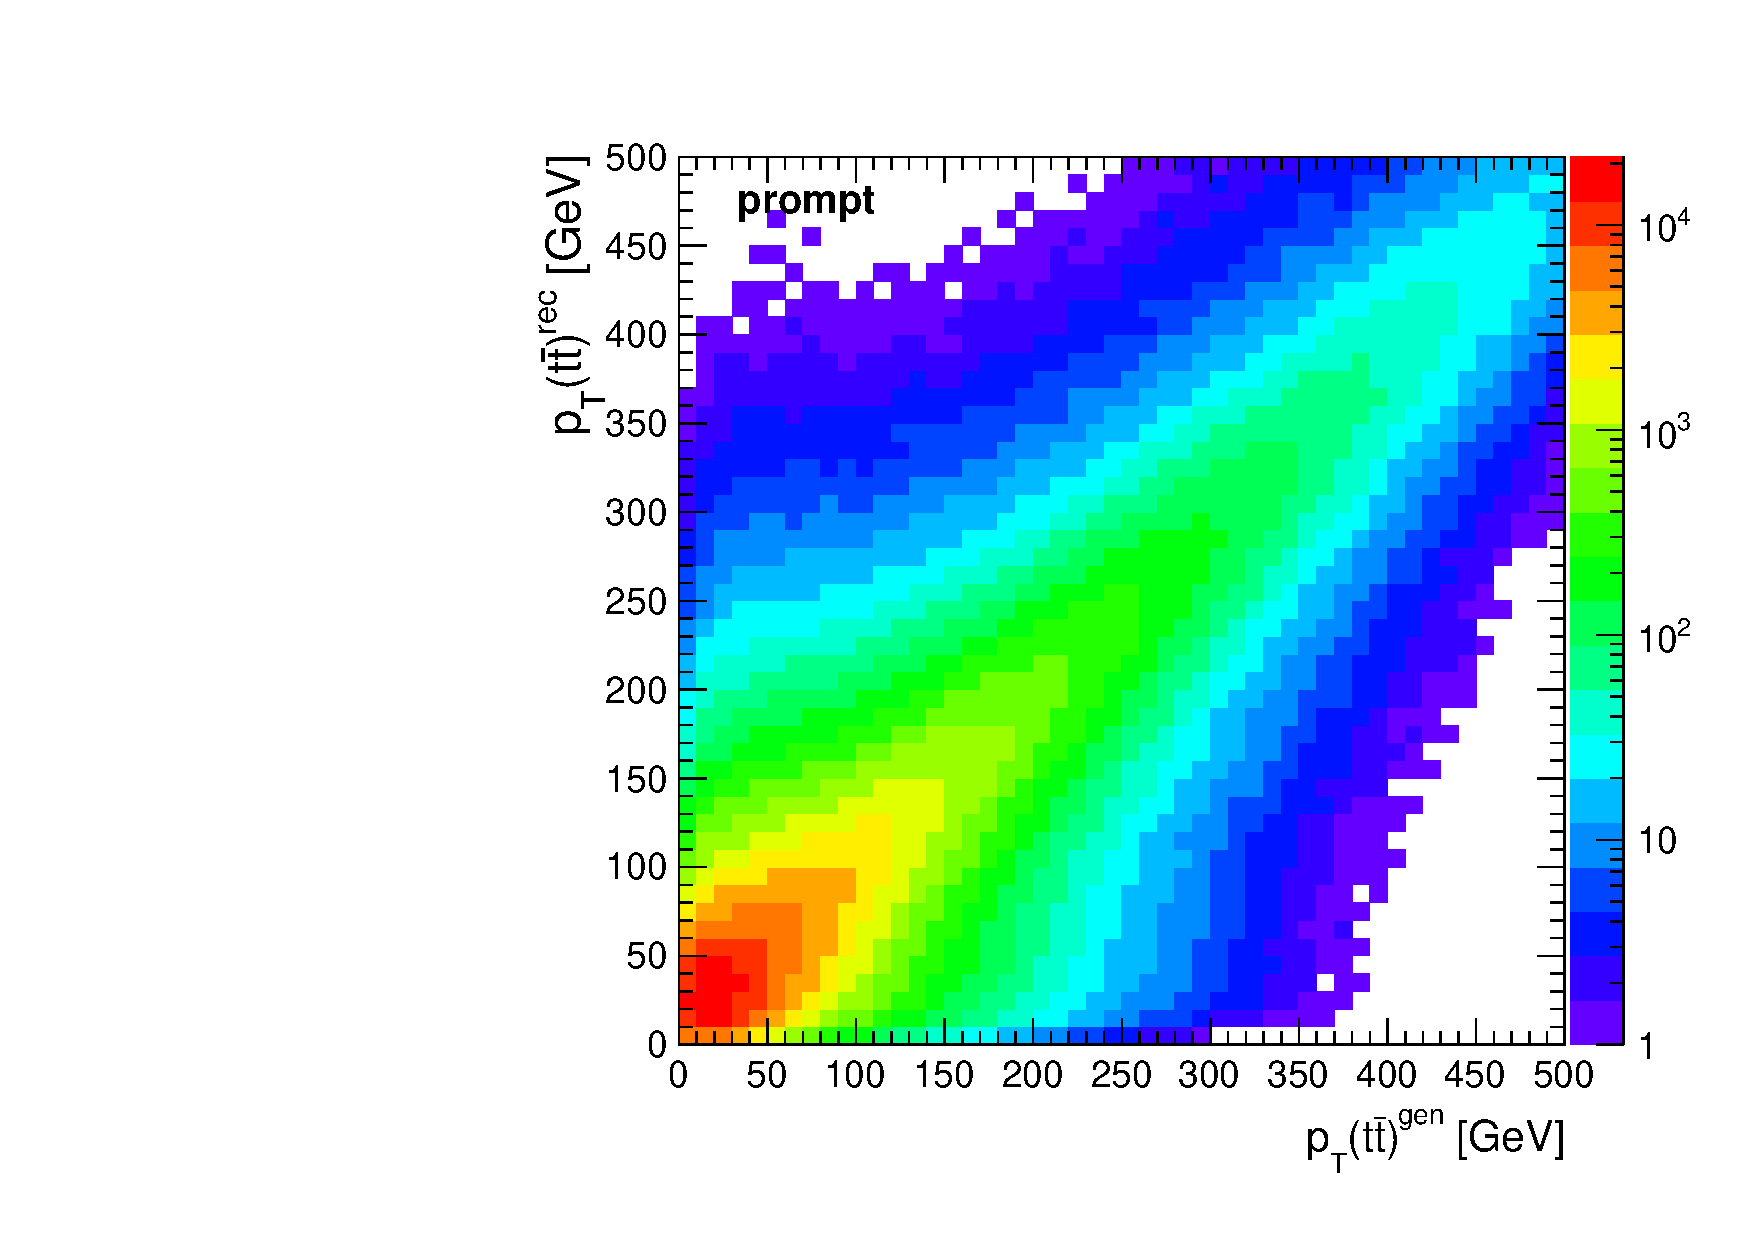
\includegraphics[width=0.30\textwidth]{fig_fullRun2UL/KinRecoResolutions/ttbar_pT_genreco_prompt.pdf}
    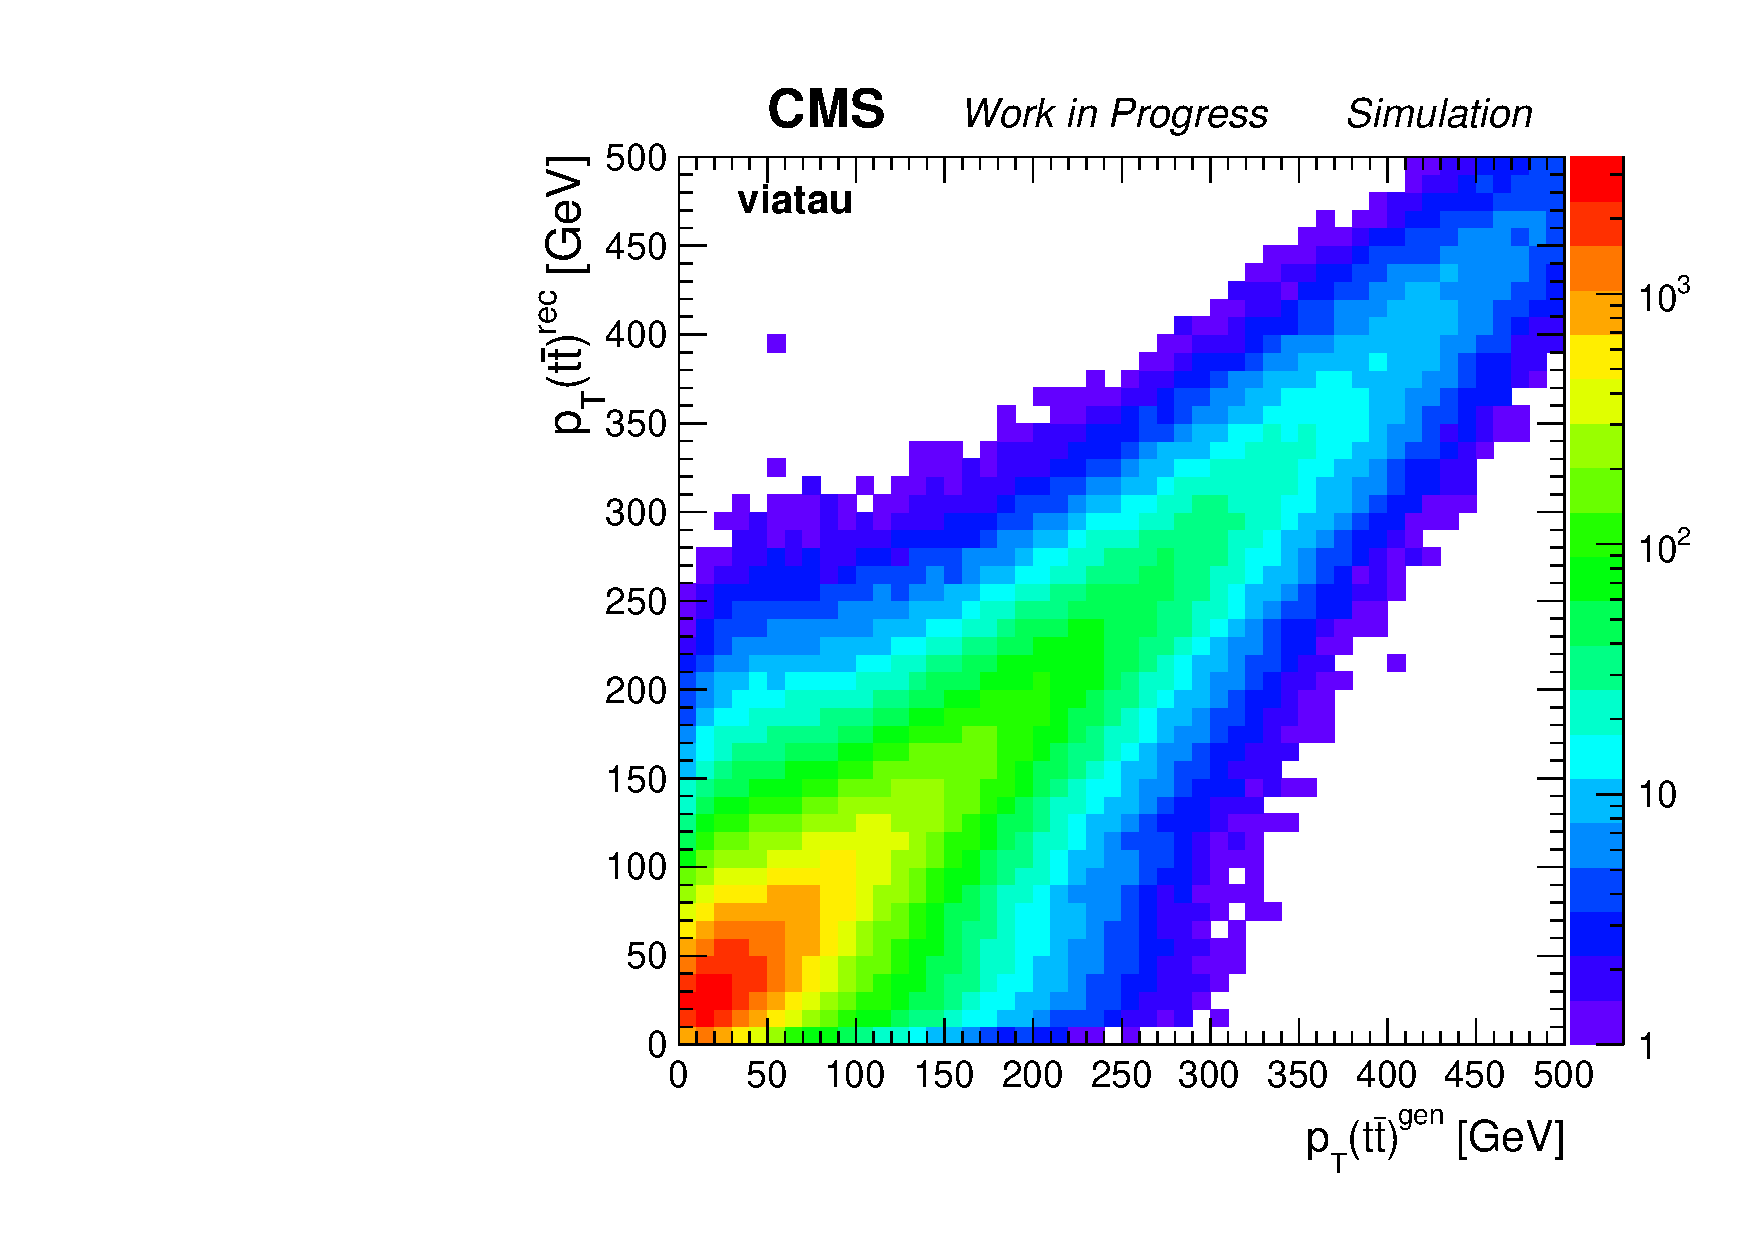
\includegraphics[width=0.30\textwidth]{fig_fullRun2UL/KinRecoResolutions/ttbar_pT_genreco_viatau.pdf}\\
    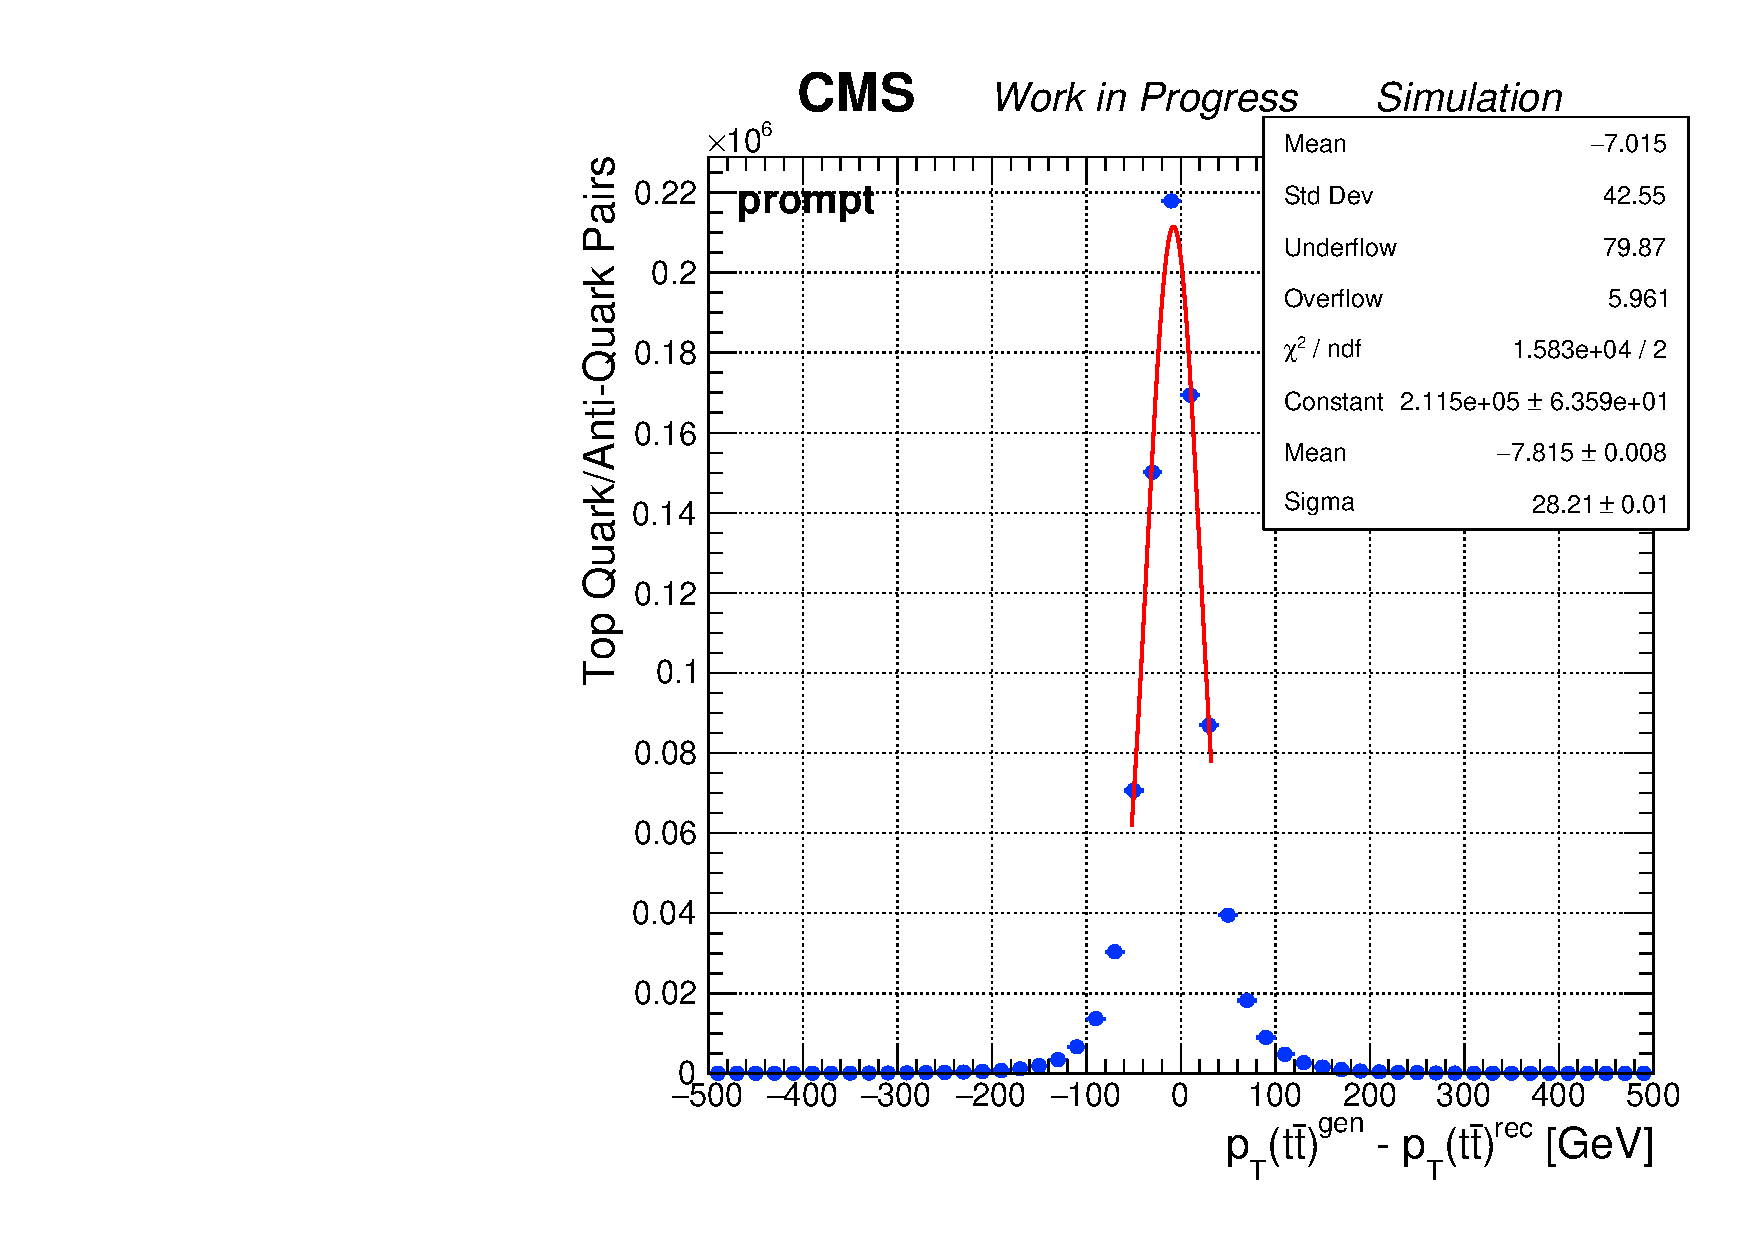
\includegraphics[width=0.30\textwidth]{fig_fullRun2UL/KinRecoResolutions/ttbar_pT_residual_prompt.pdf}
    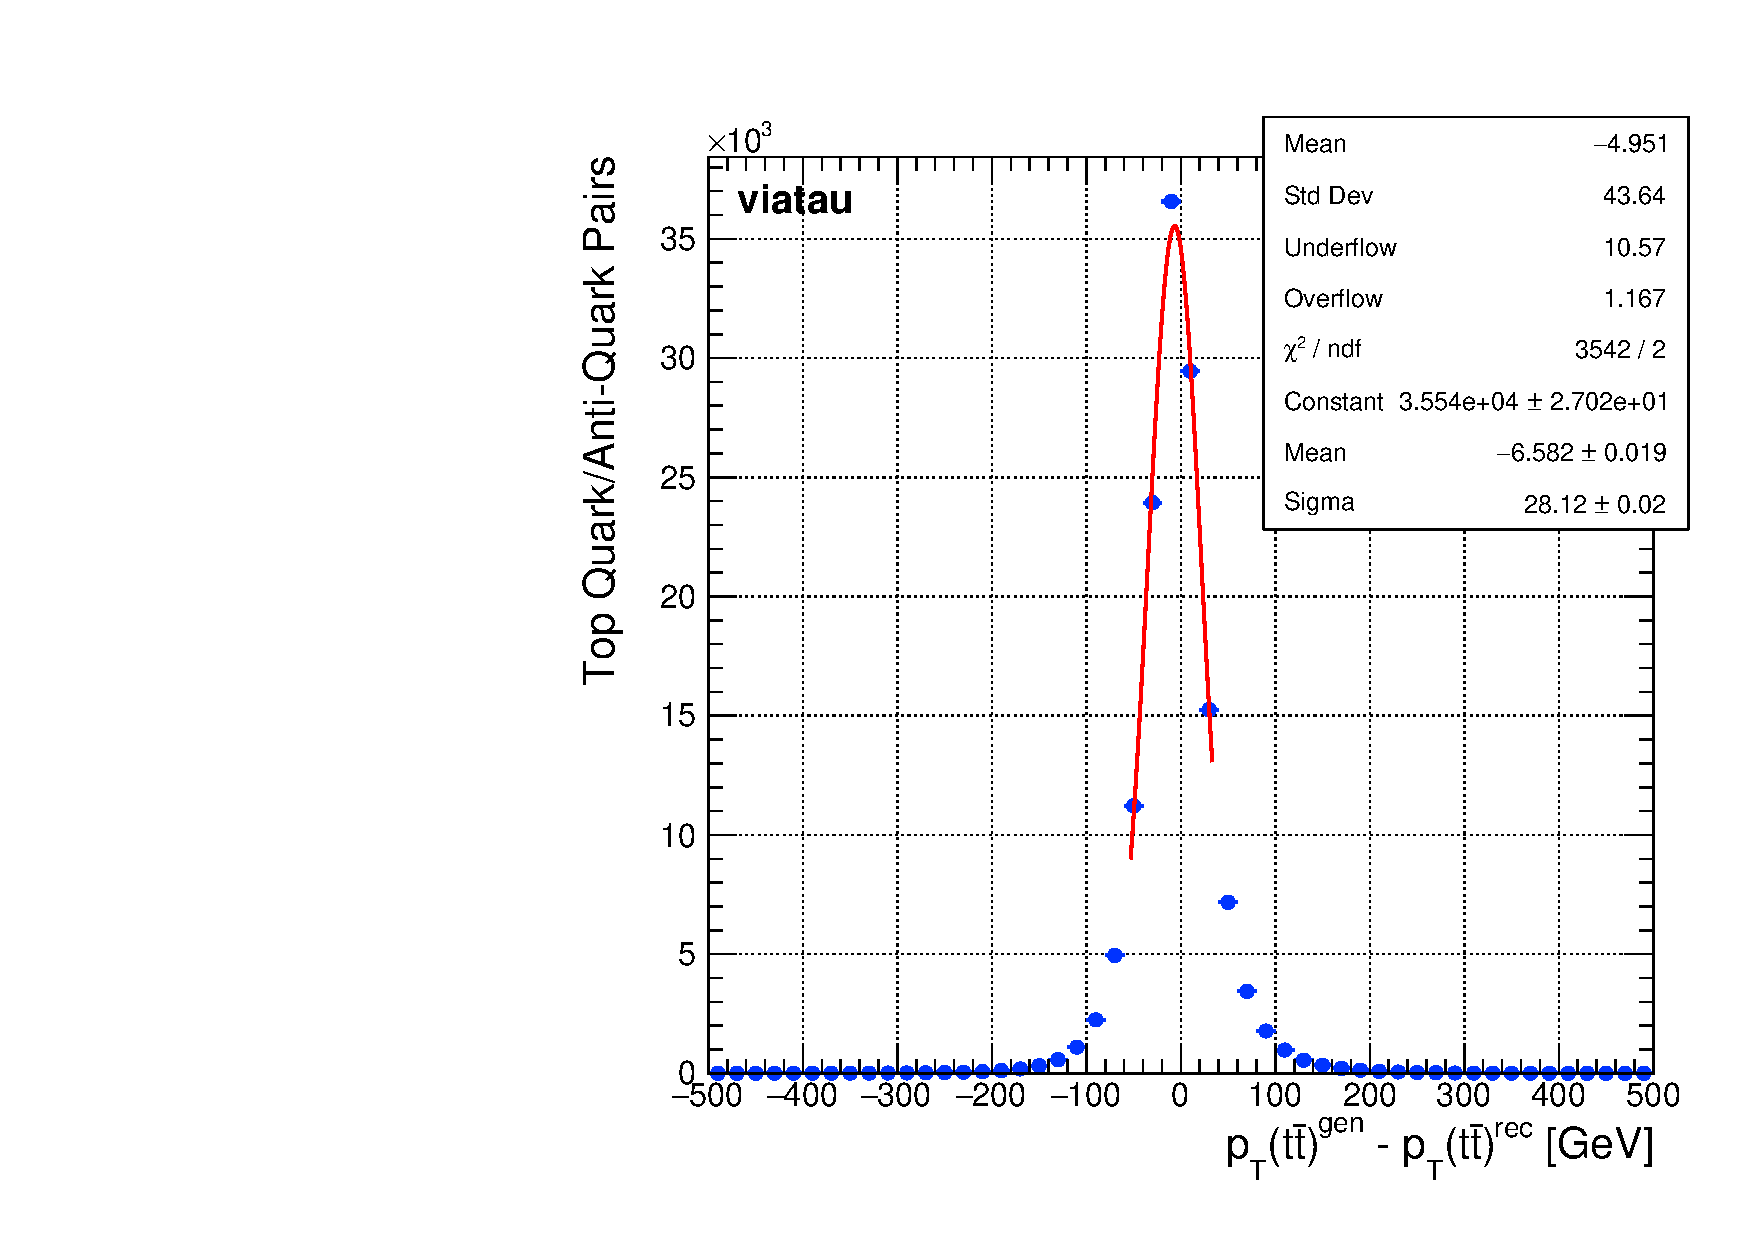
\includegraphics[width=0.30\textwidth]{fig_fullRun2UL/KinRecoResolutions/ttbar_pT_residual_viatau.pdf}\\
    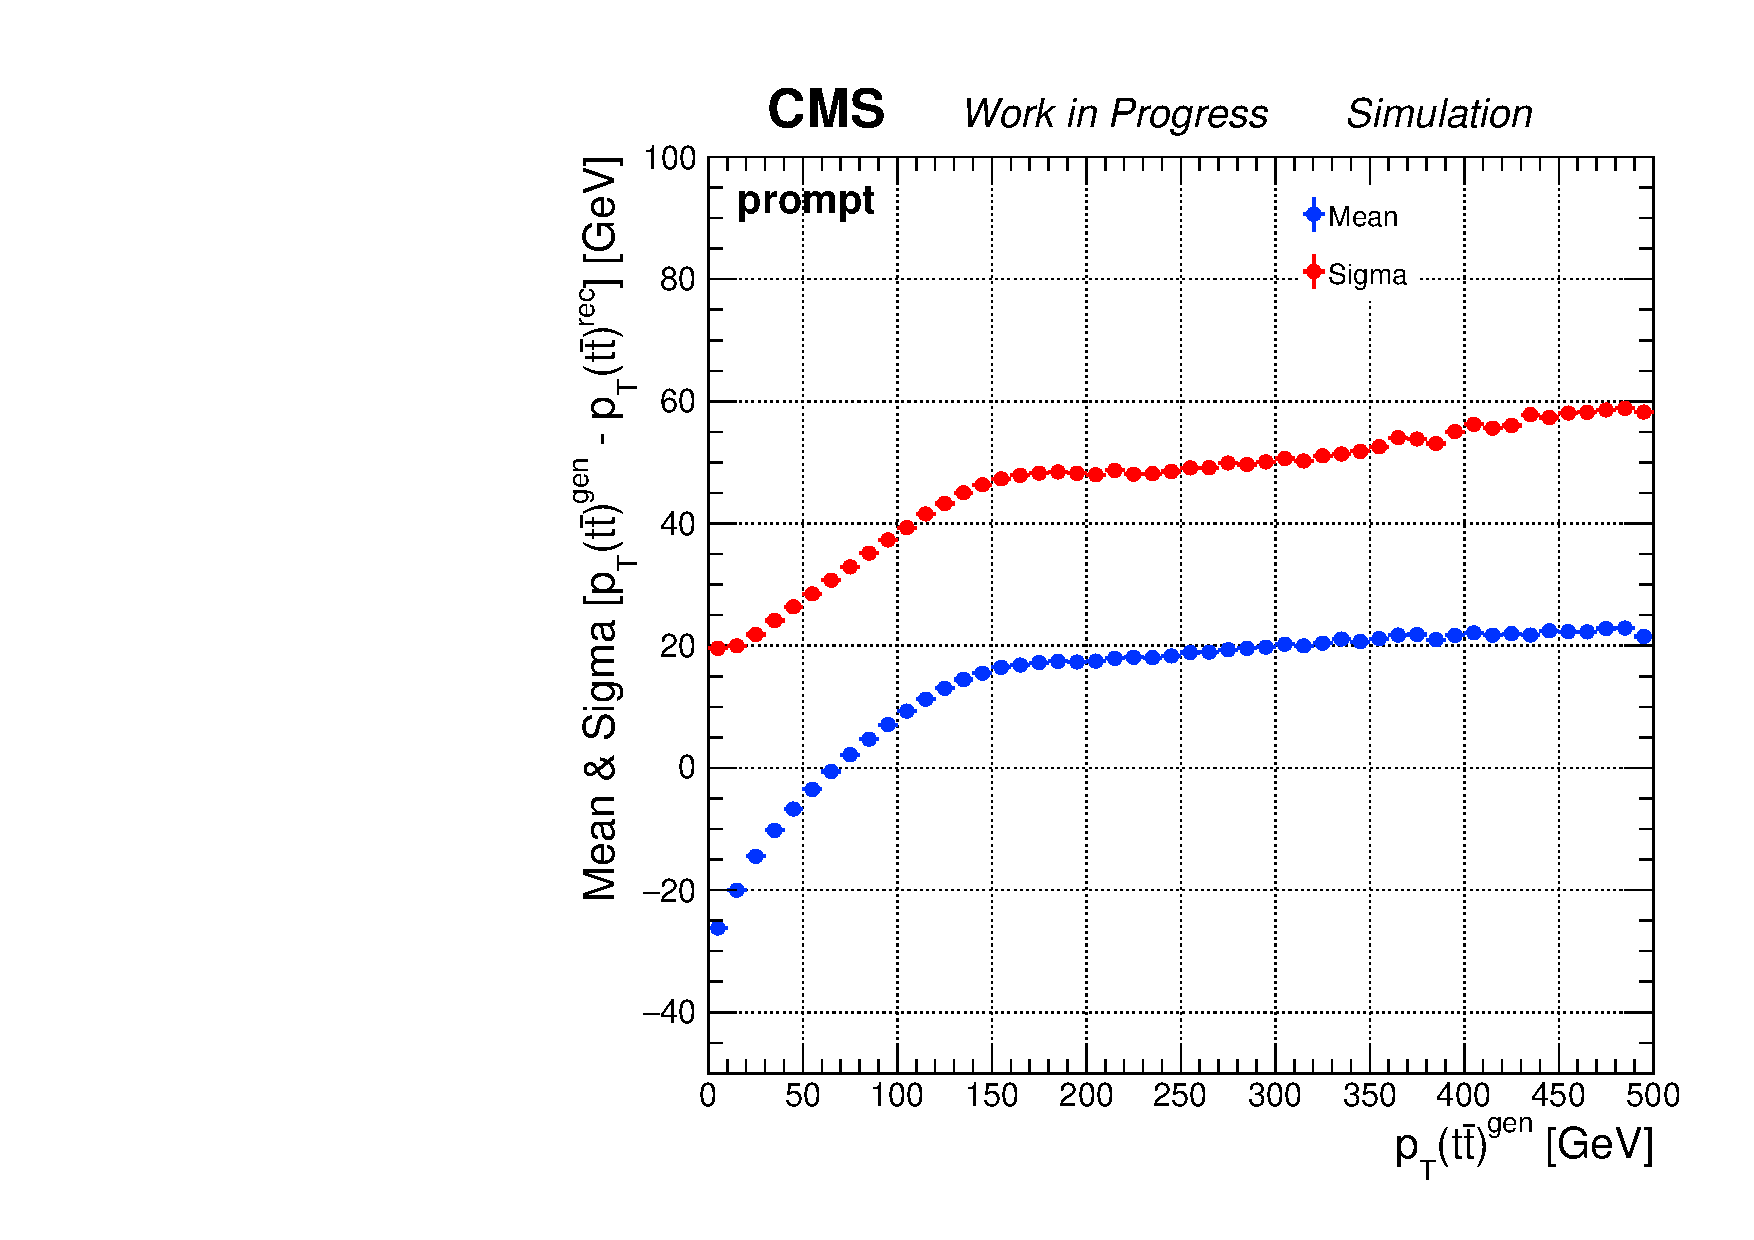
\includegraphics[width=0.30\textwidth]{fig_fullRun2UL/KinRecoResolutions/ttbar_pT_multiresidual_prompt.pdf}
    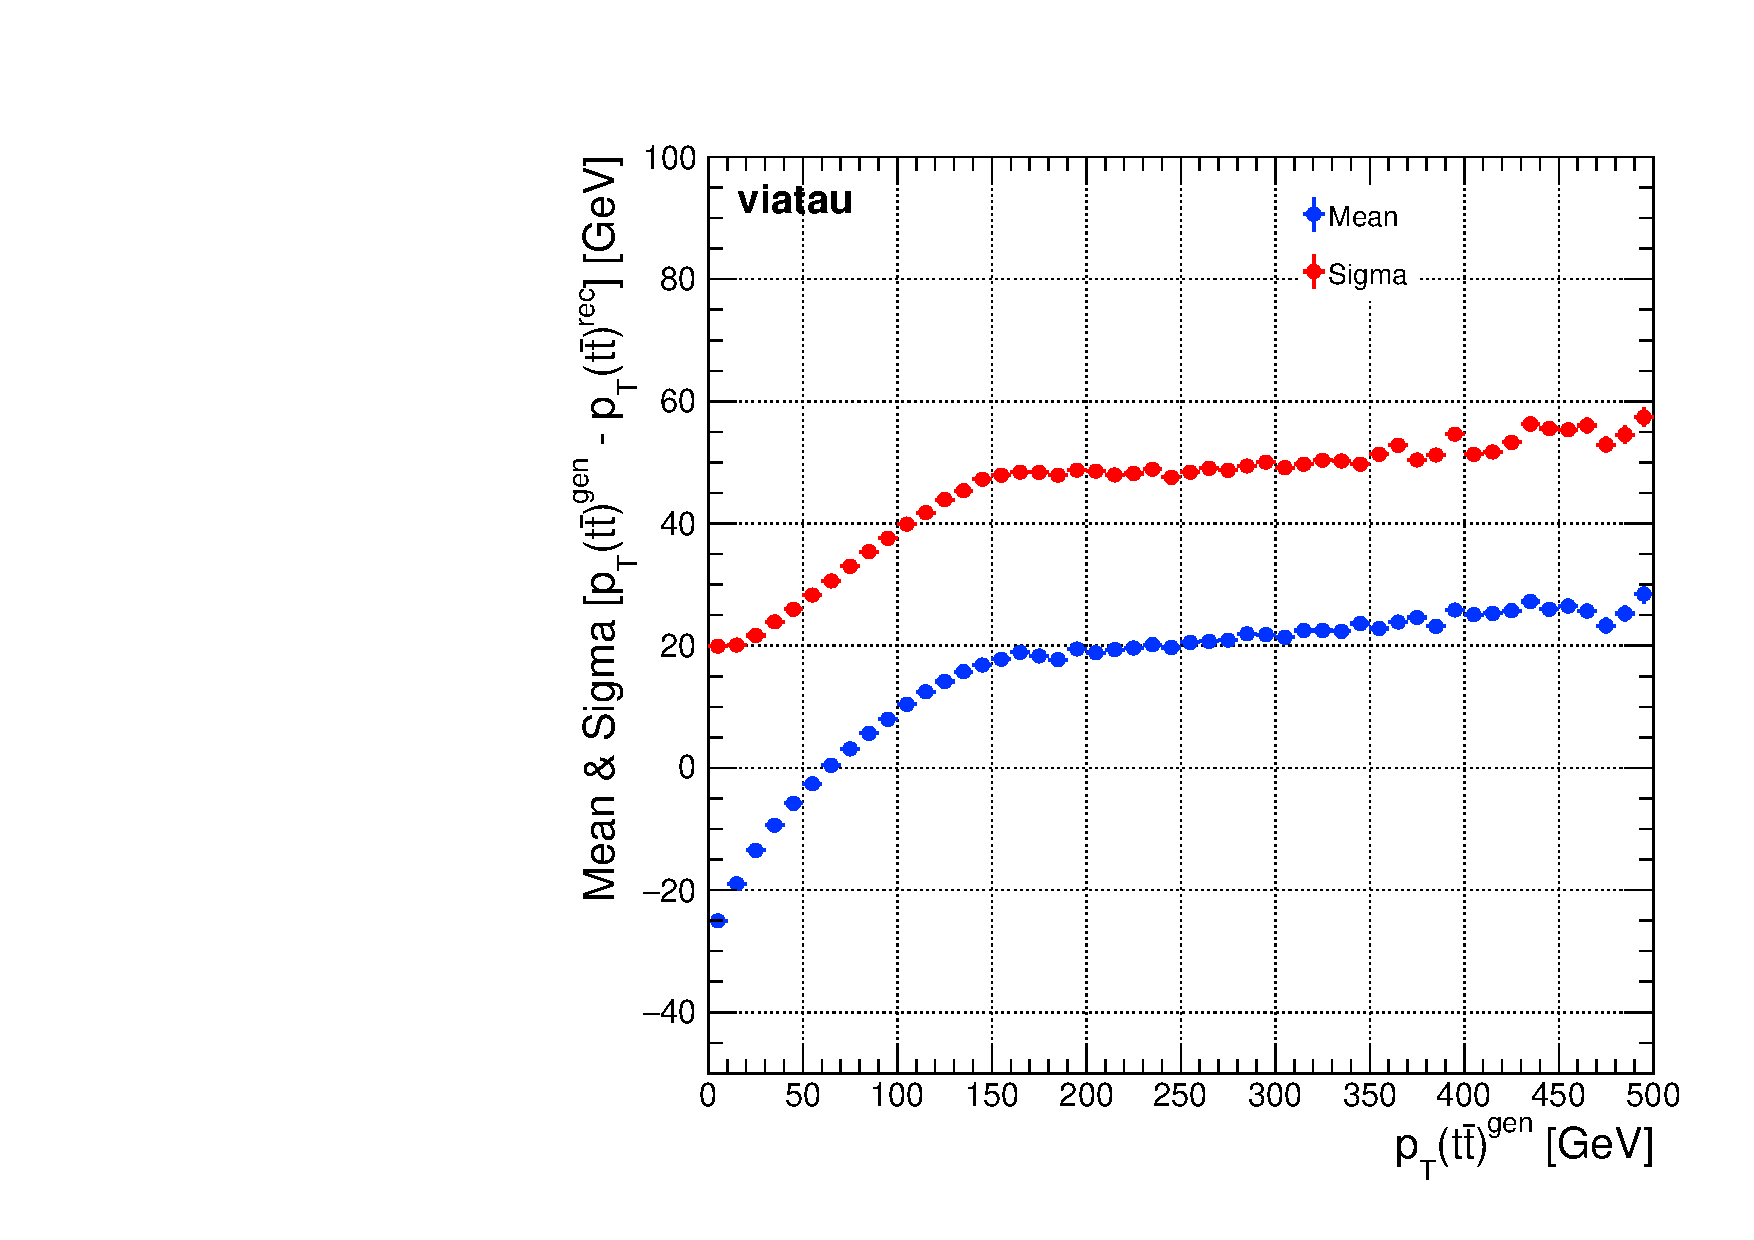
\includegraphics[width=0.30\textwidth]{fig_fullRun2UL/KinRecoResolutions/ttbar_pT_multiresidual_viatau.pdf}\\
    \caption{\small Top: True and reconstructed \pttt\ obtained for prompt (left) and via tau (right) \ttbar dilepton events.
    Middle: The difference between true and reconstructed \pttt\ in bins of true \pttt\ (fitted with a Gaussian function for illustration).
    Bottom: The differential mean and sigma from Gaussian fits, with respect to true \pttt, of the difference between true and reconstructed \pttt\ obtained for prompt and via tau \ttbar dilepton events.
    The simulated samples are normalized to an integrated luminosity of \lumivalueRuniiUL.}
    \label{fig:kinrec:resolution-pttt}
 \end{center}
\end{figure}

\begin{figure}
  \begin{center}
    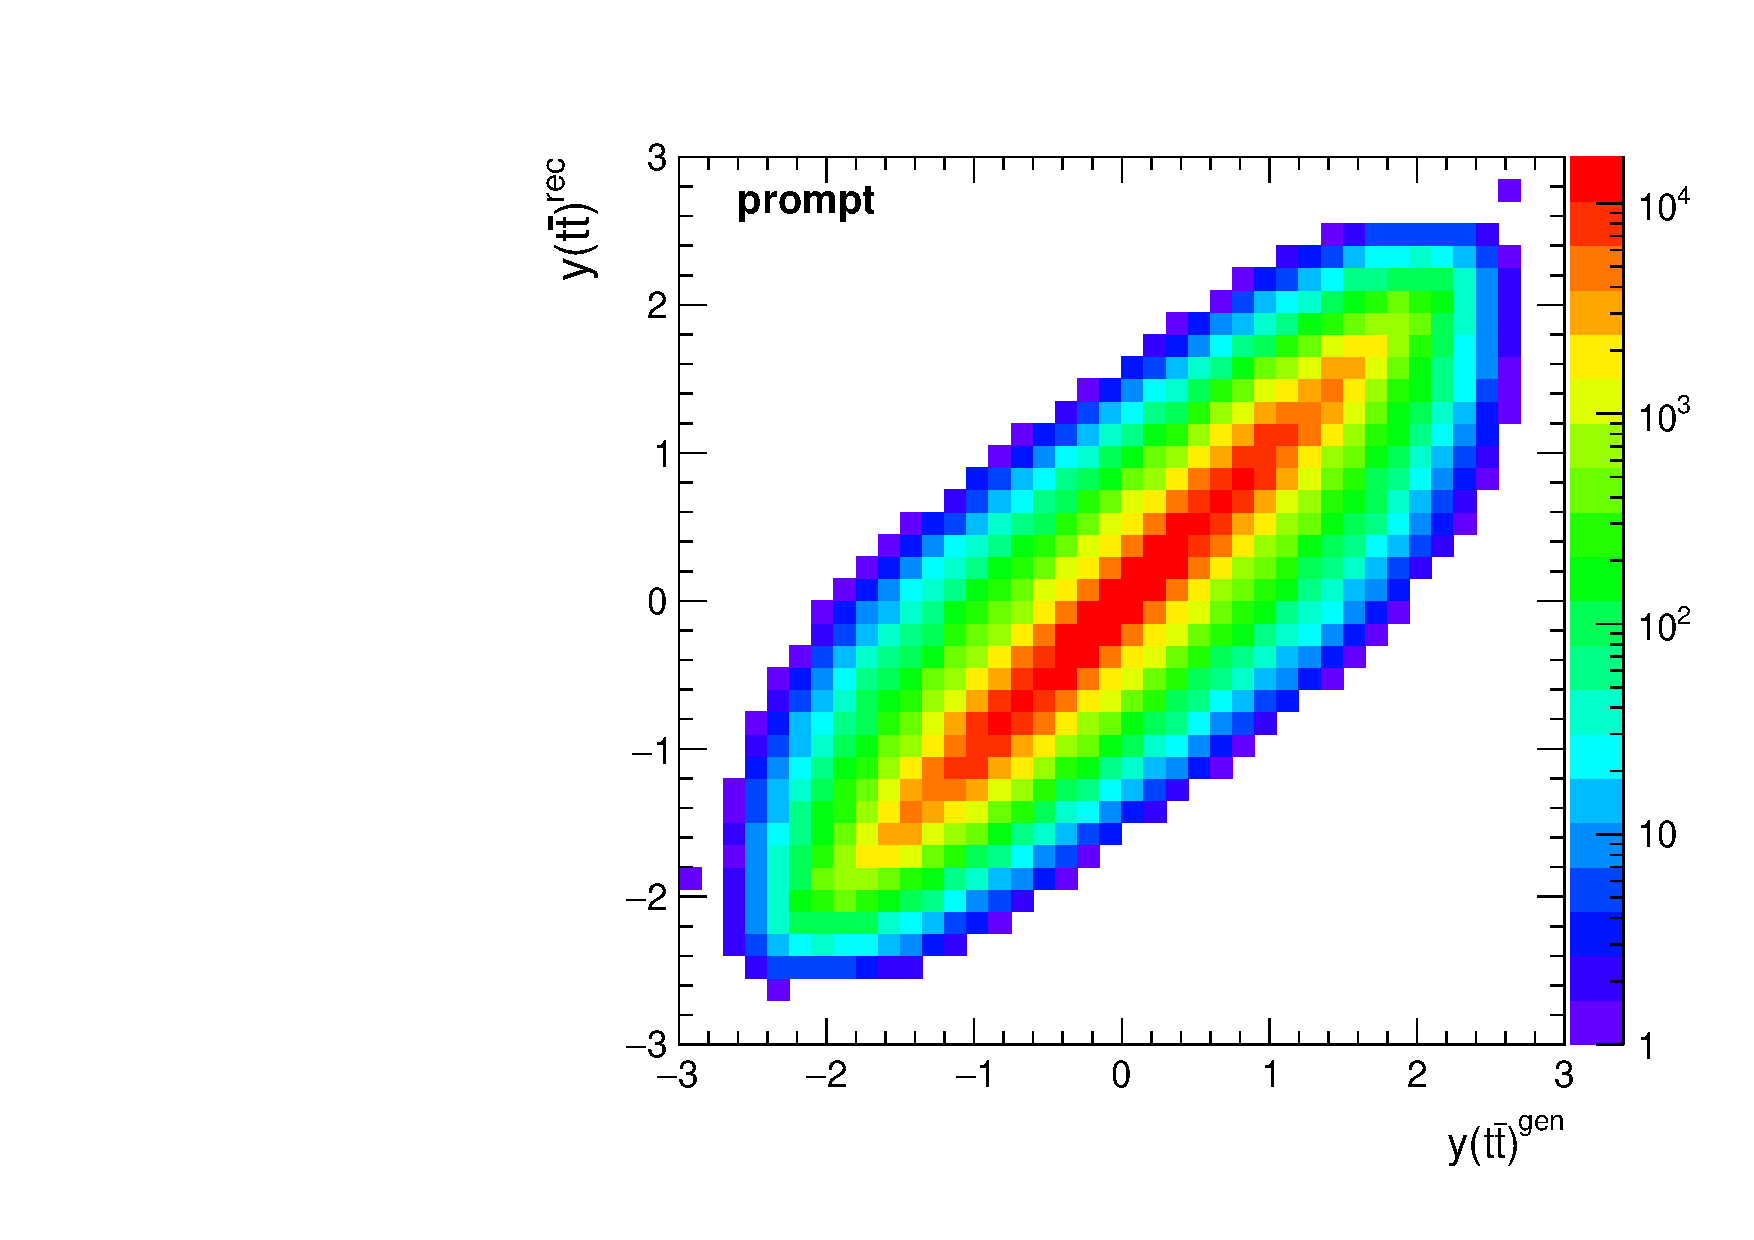
\includegraphics[width=0.30\textwidth]{fig_fullRun2UL/KinRecoResolutions/ttbar_rapidity_genreco_prompt.pdf}
    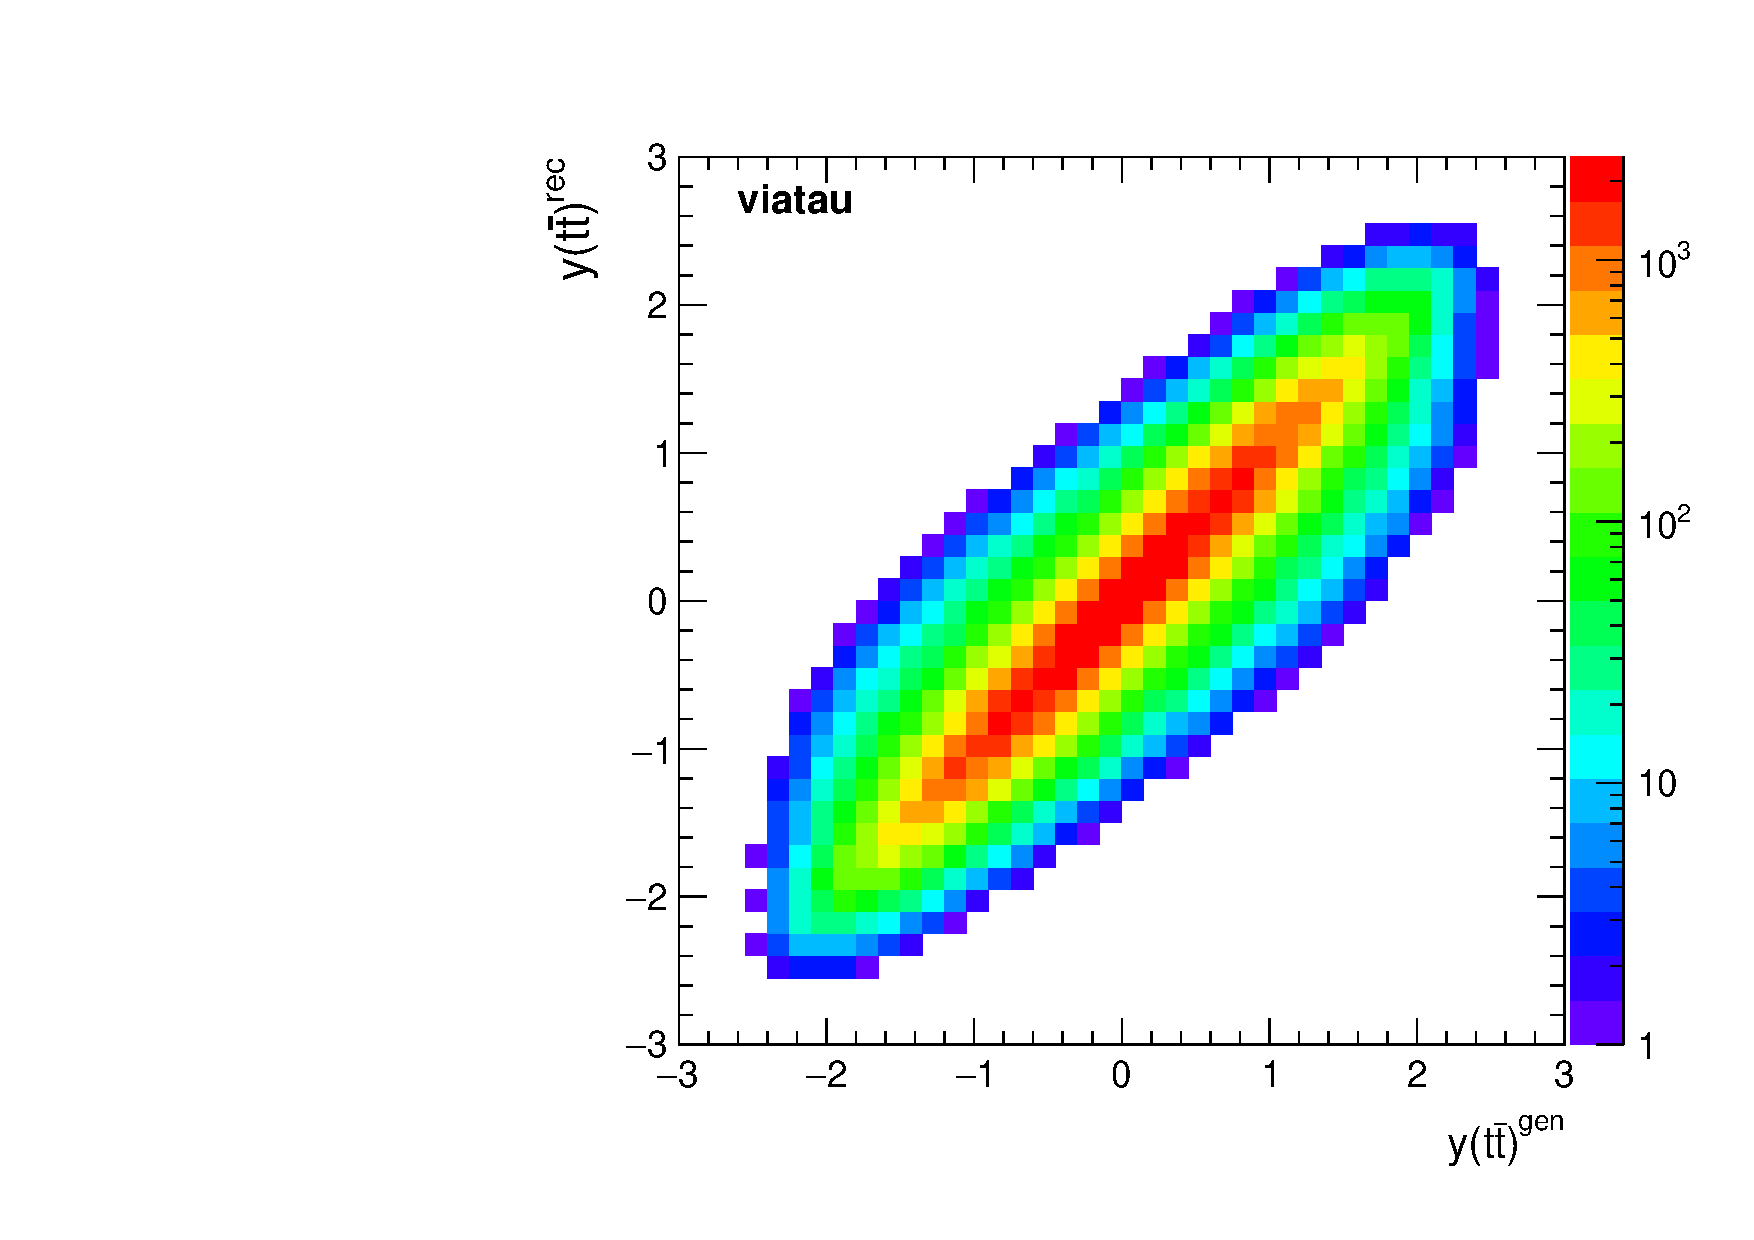
\includegraphics[width=0.30\textwidth]{fig_fullRun2UL/KinRecoResolutions/ttbar_rapidity_genreco_viatau.pdf}\\
    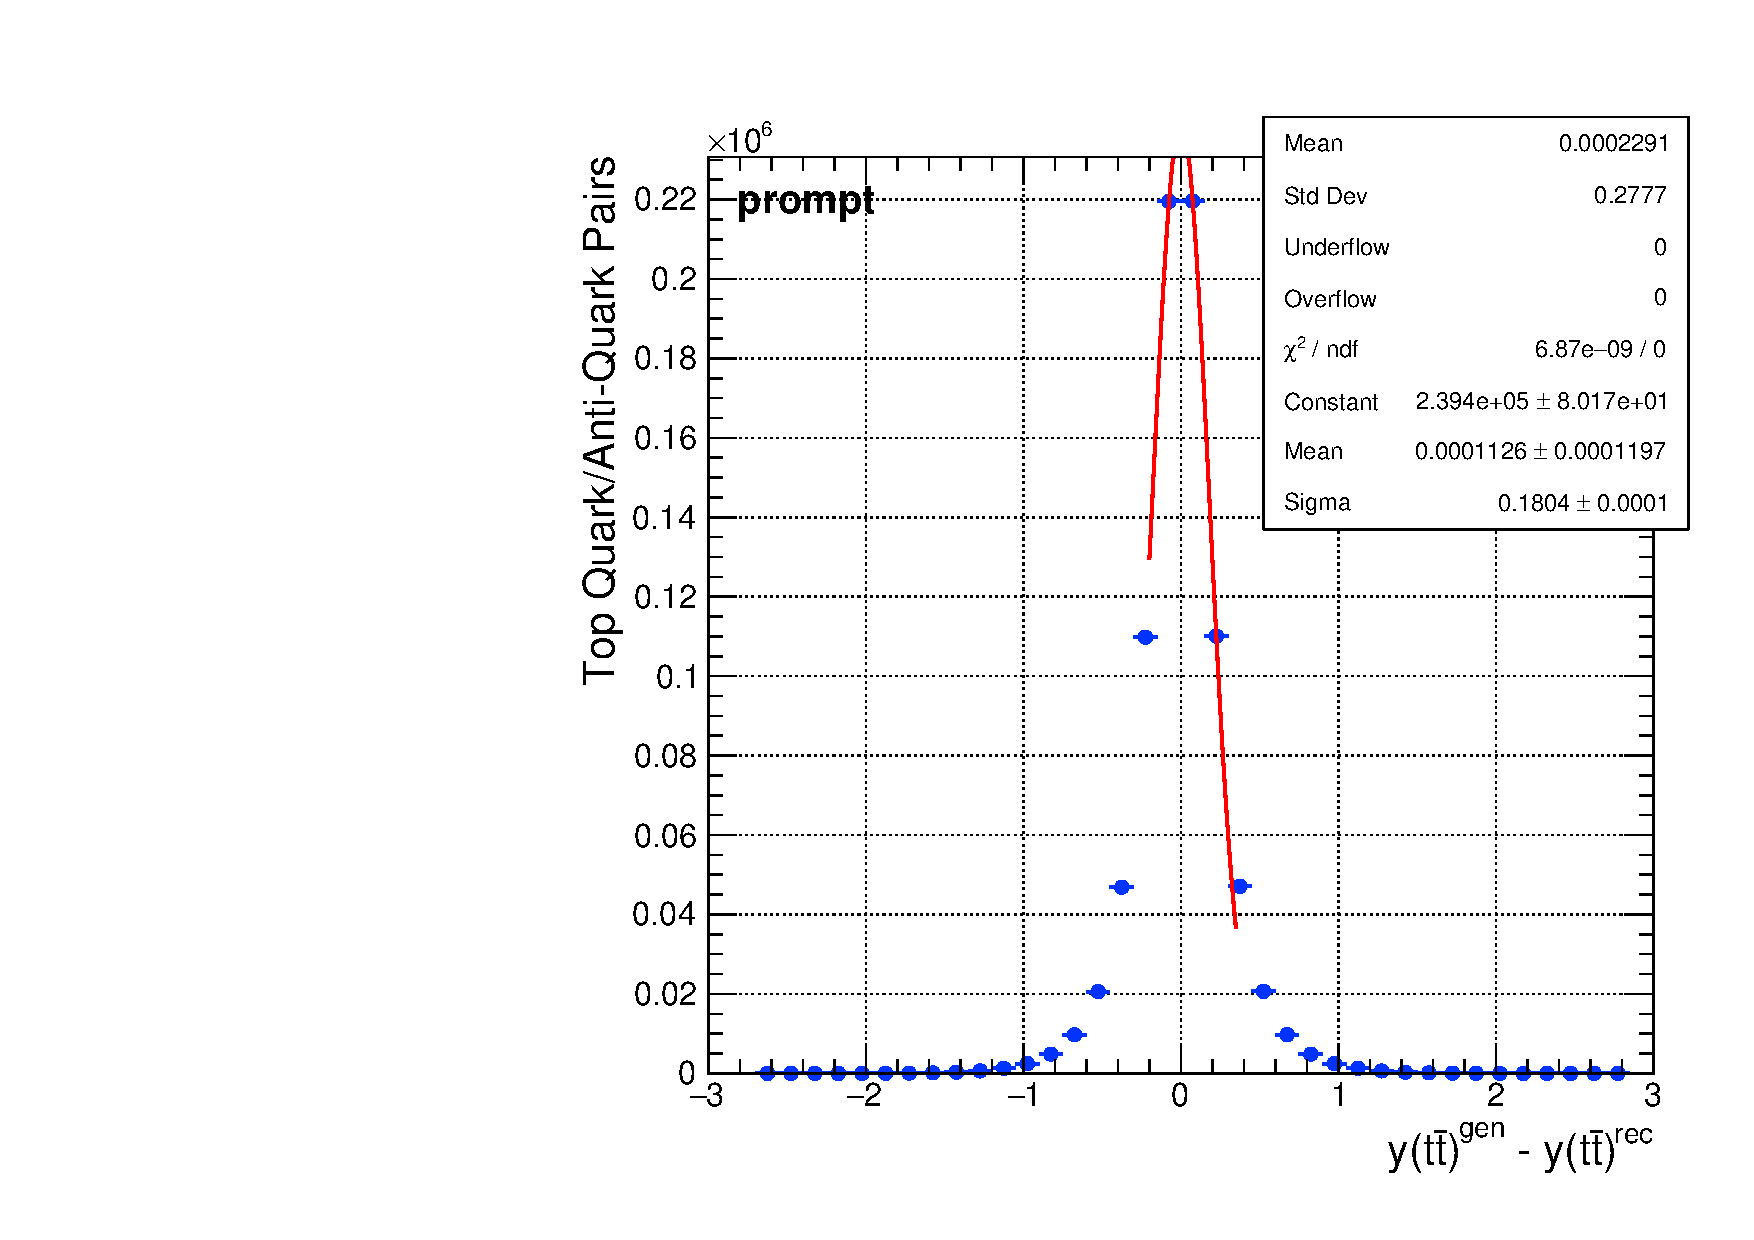
\includegraphics[width=0.30\textwidth]{fig_fullRun2UL/KinRecoResolutions/ttbar_rapidity_residual_prompt.pdf}
    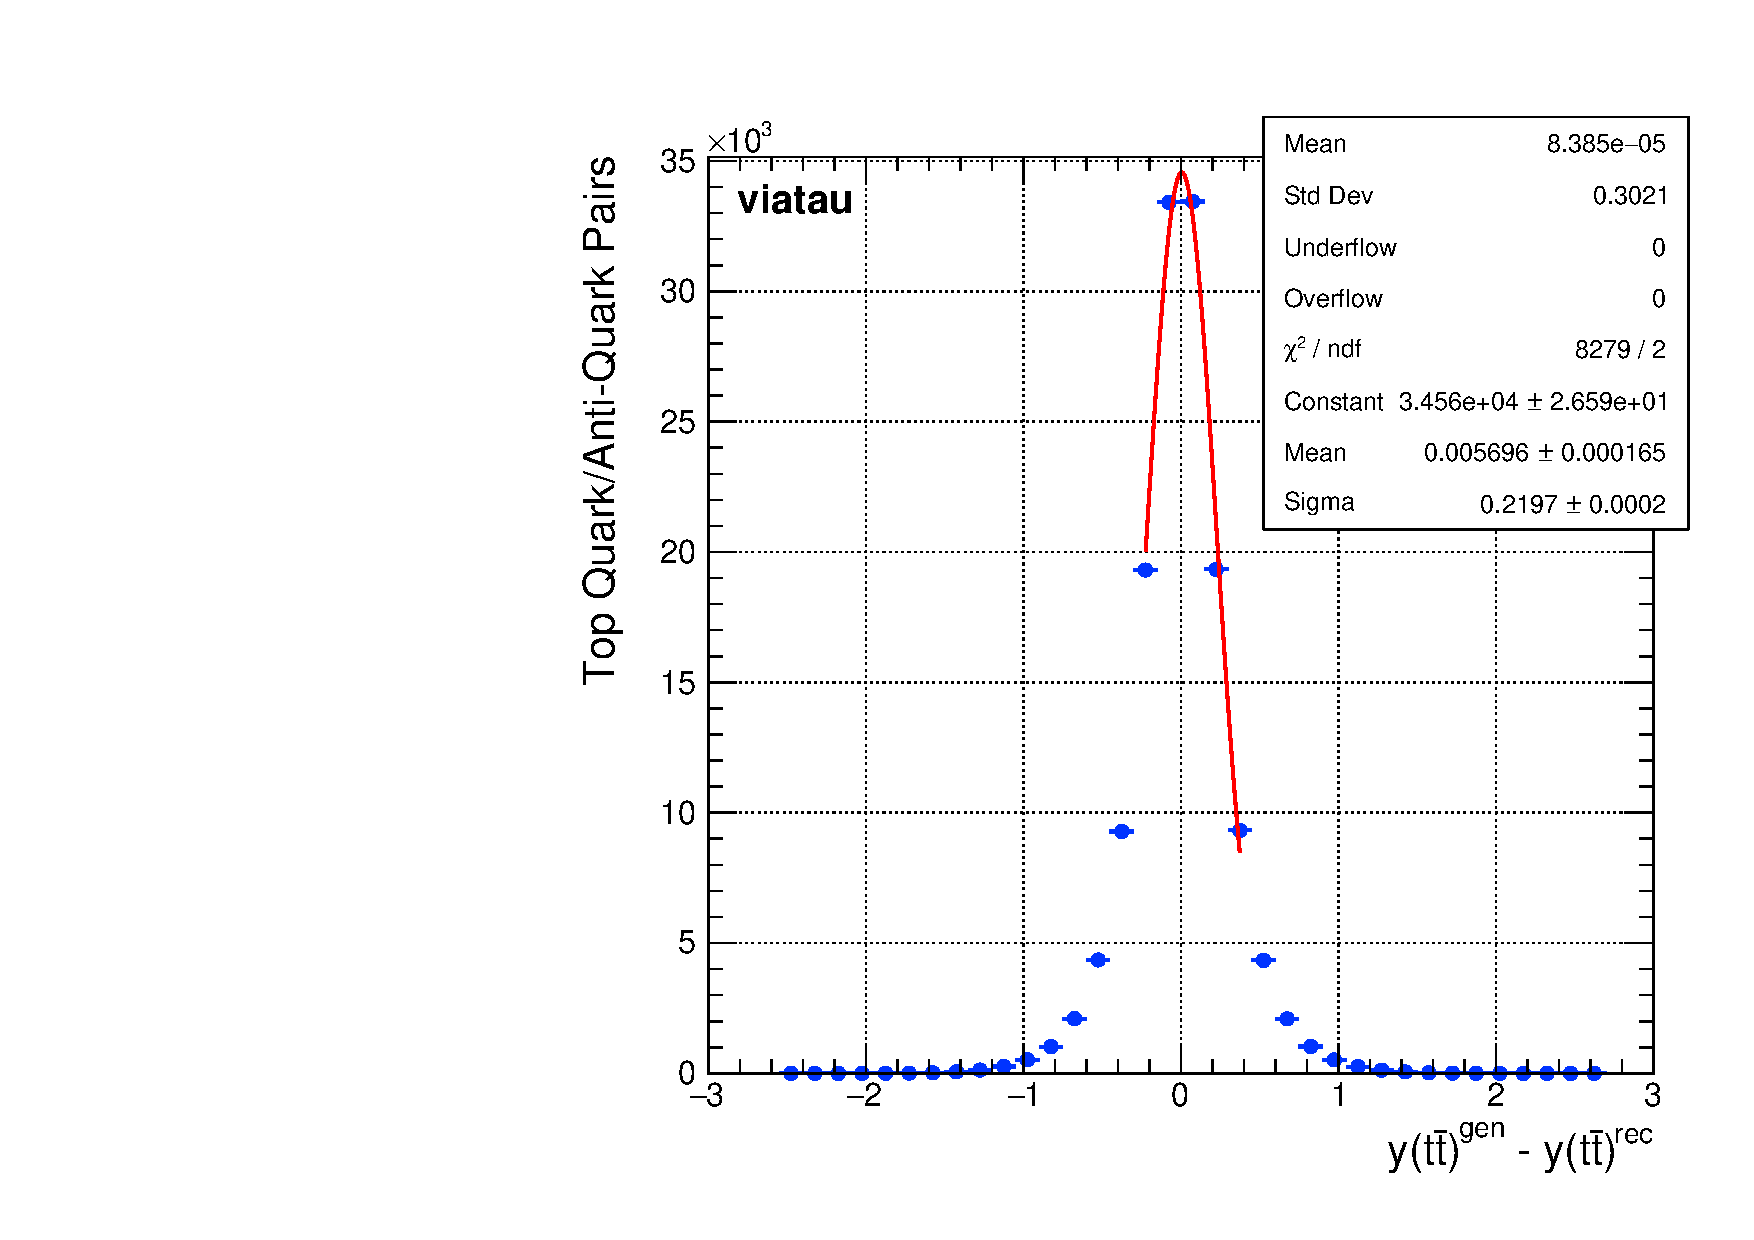
\includegraphics[width=0.30\textwidth]{fig_fullRun2UL/KinRecoResolutions/ttbar_rapidity_residual_viatau.pdf}\\
    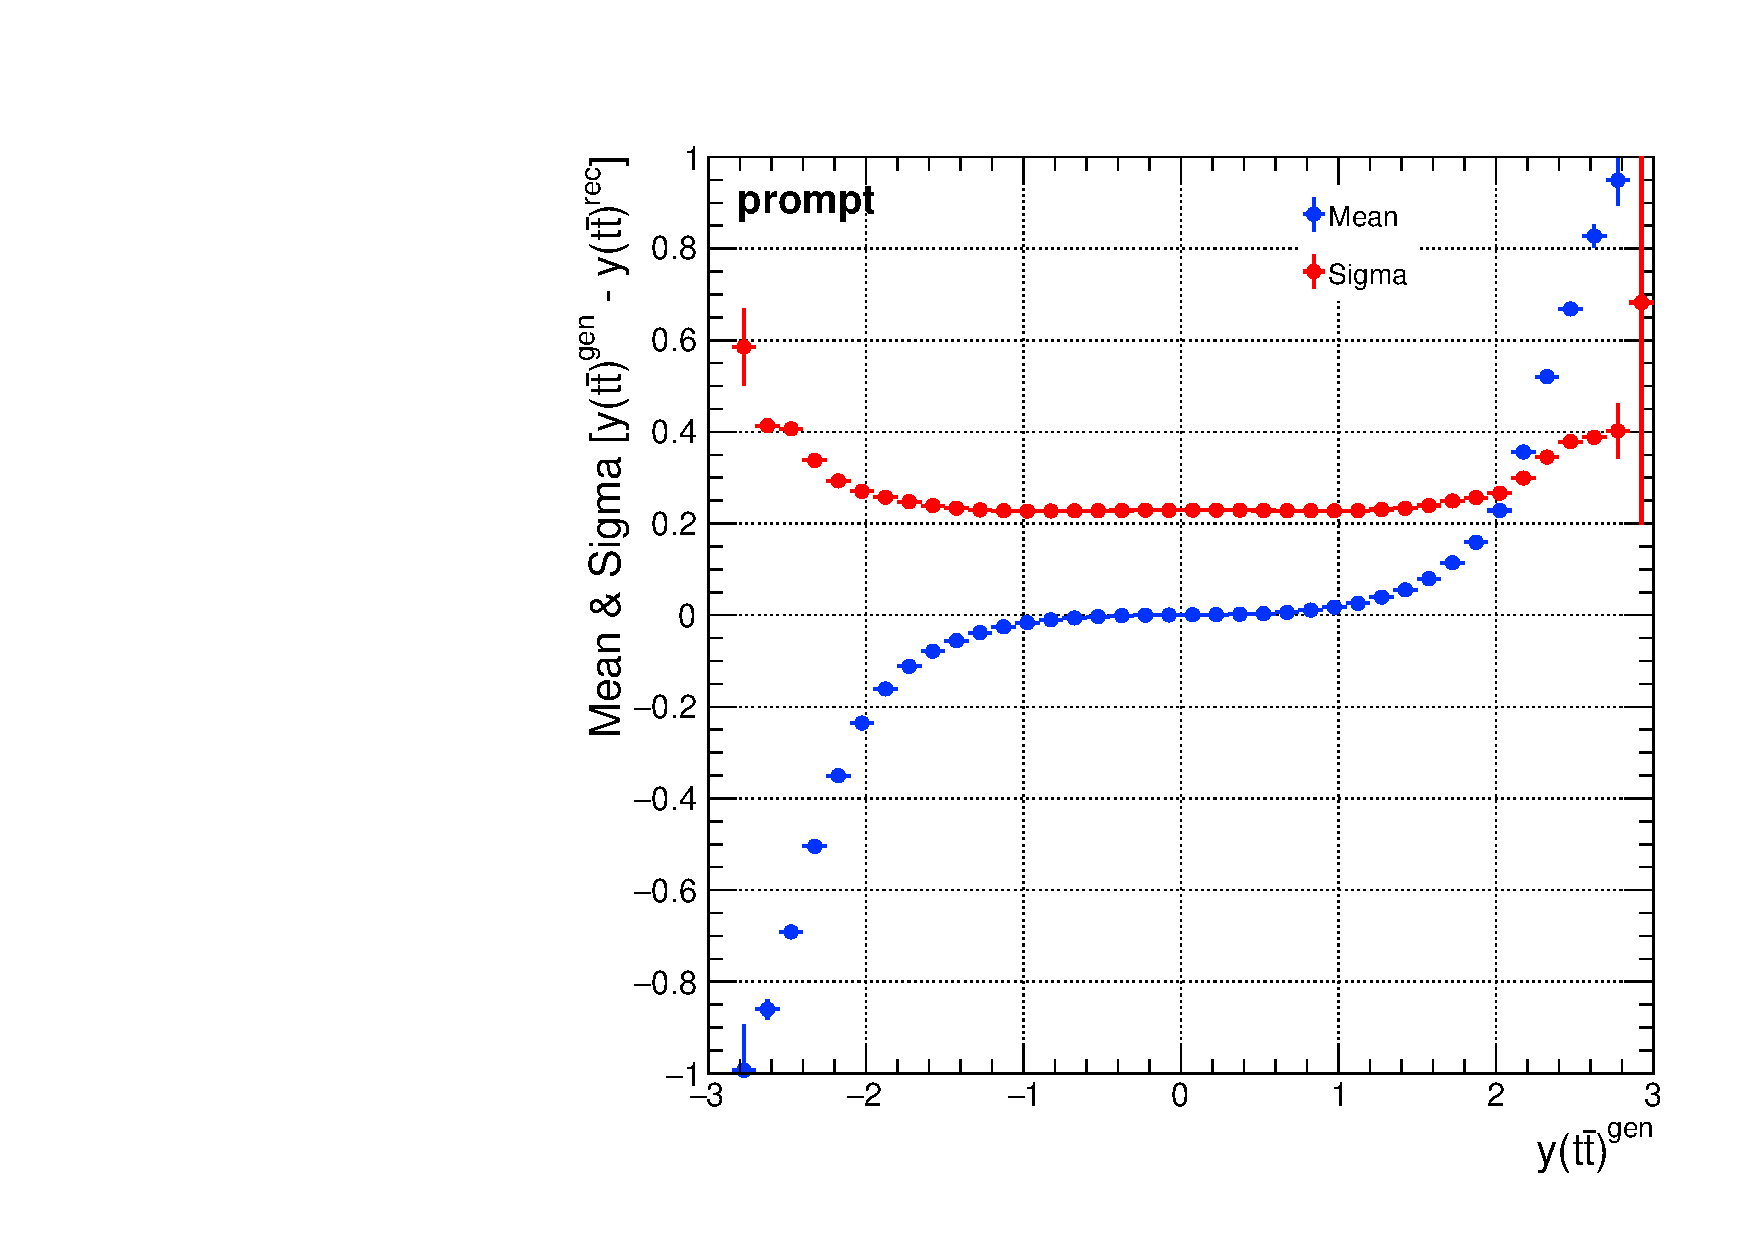
\includegraphics[width=0.30\textwidth]{fig_fullRun2UL/KinRecoResolutions/ttbar_rapidity_multiresidual_prompt.pdf}
    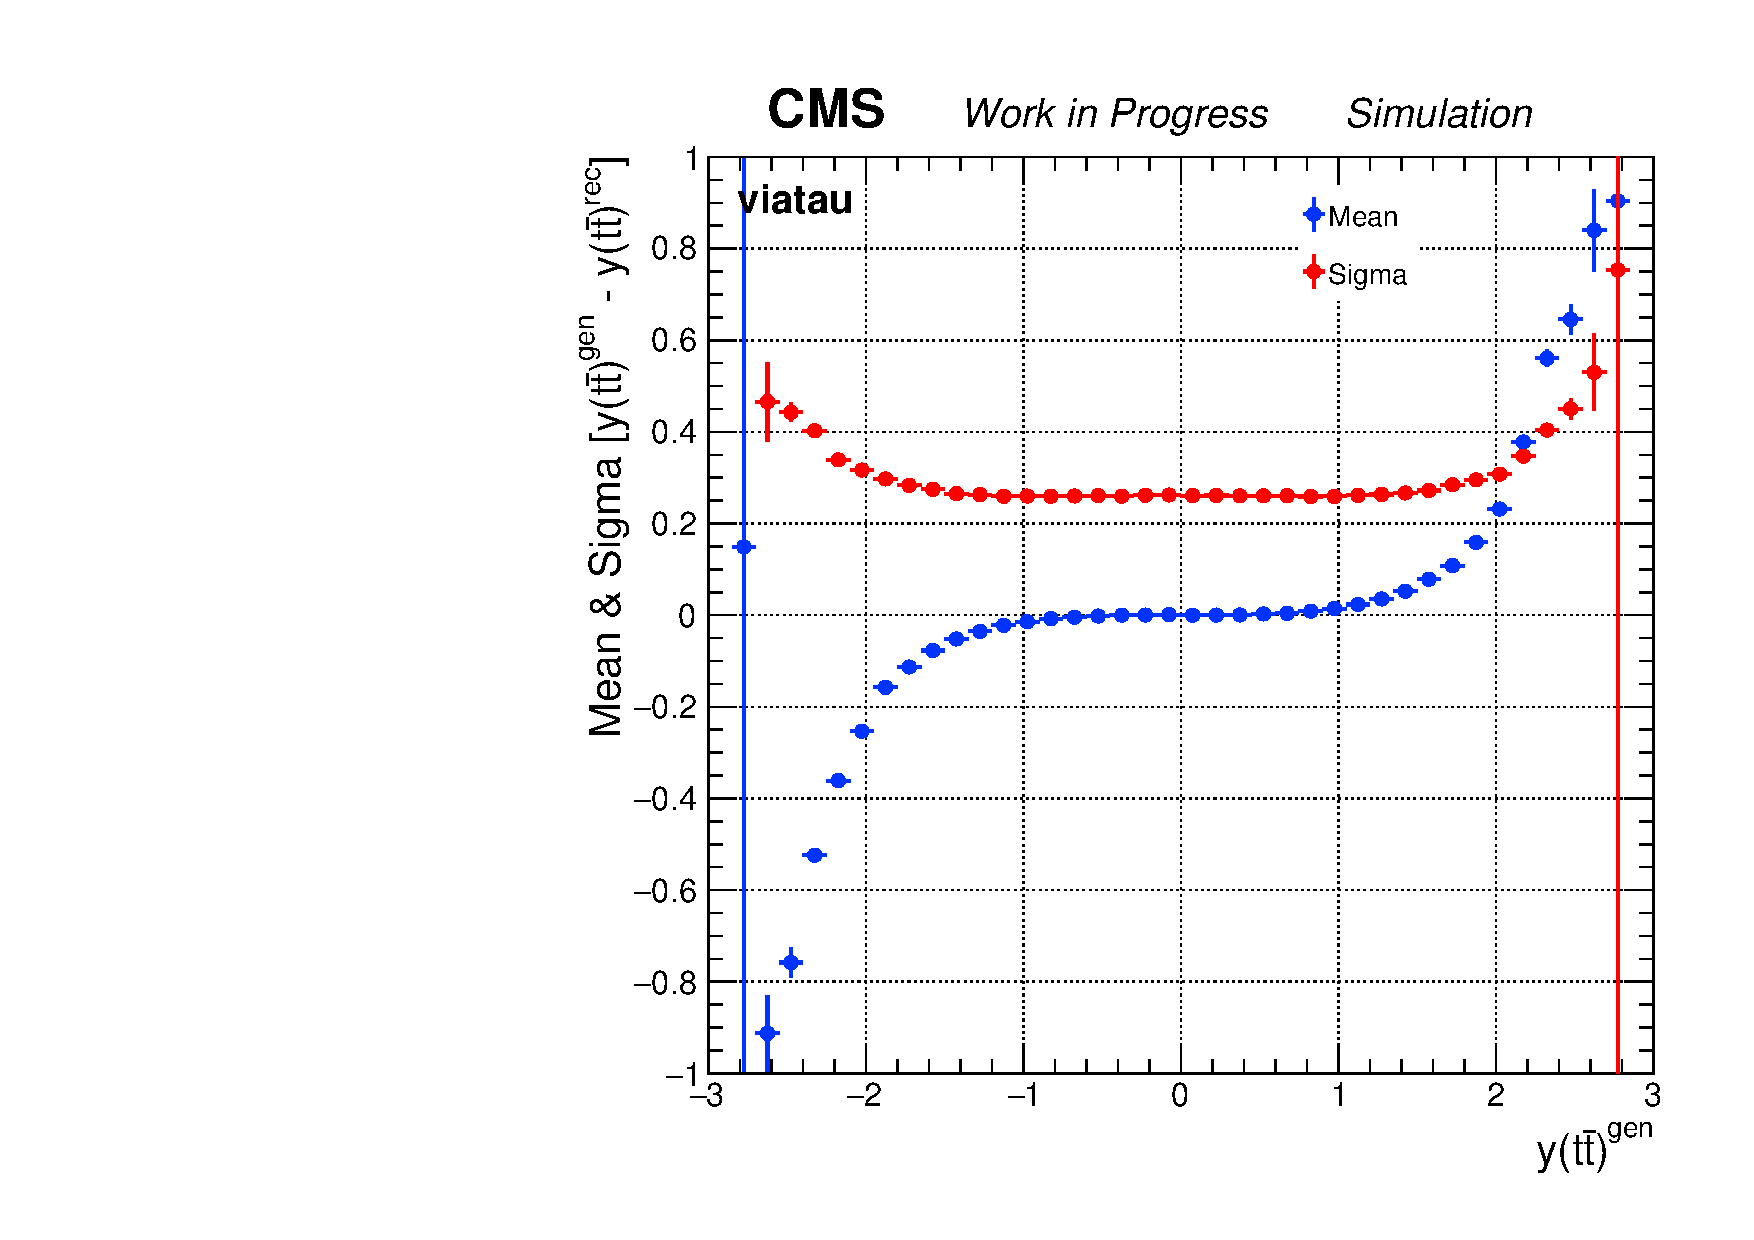
\includegraphics[width=0.30\textwidth]{fig_fullRun2UL/KinRecoResolutions/ttbar_rapidity_multiresidual_viatau.pdf}\\
    \caption{\small Top: True and reconstructed \ytt\ obtained for prompt (left) and via tau (right) \ttbar dilepton events.
    Middle: The difference between true and reconstructed \ytt\ in bins of true \ytt\ (fitted with a Gaussian function for illustration).
    Bottom: The differential mean and sigma from Gaussian fits, with respect to true \ytt, of the difference between true and reconstructed \ytt\ obtained for prompt and via tau \ttbar dilepton events.
    The simulated samples are normalized to an integrated luminosity of \lumivalueRuniiUL.}
    \label{fig:kinrec:resolution-ytt}
 \end{center}
\end{figure}

\begin{figure}
  \begin{center}
    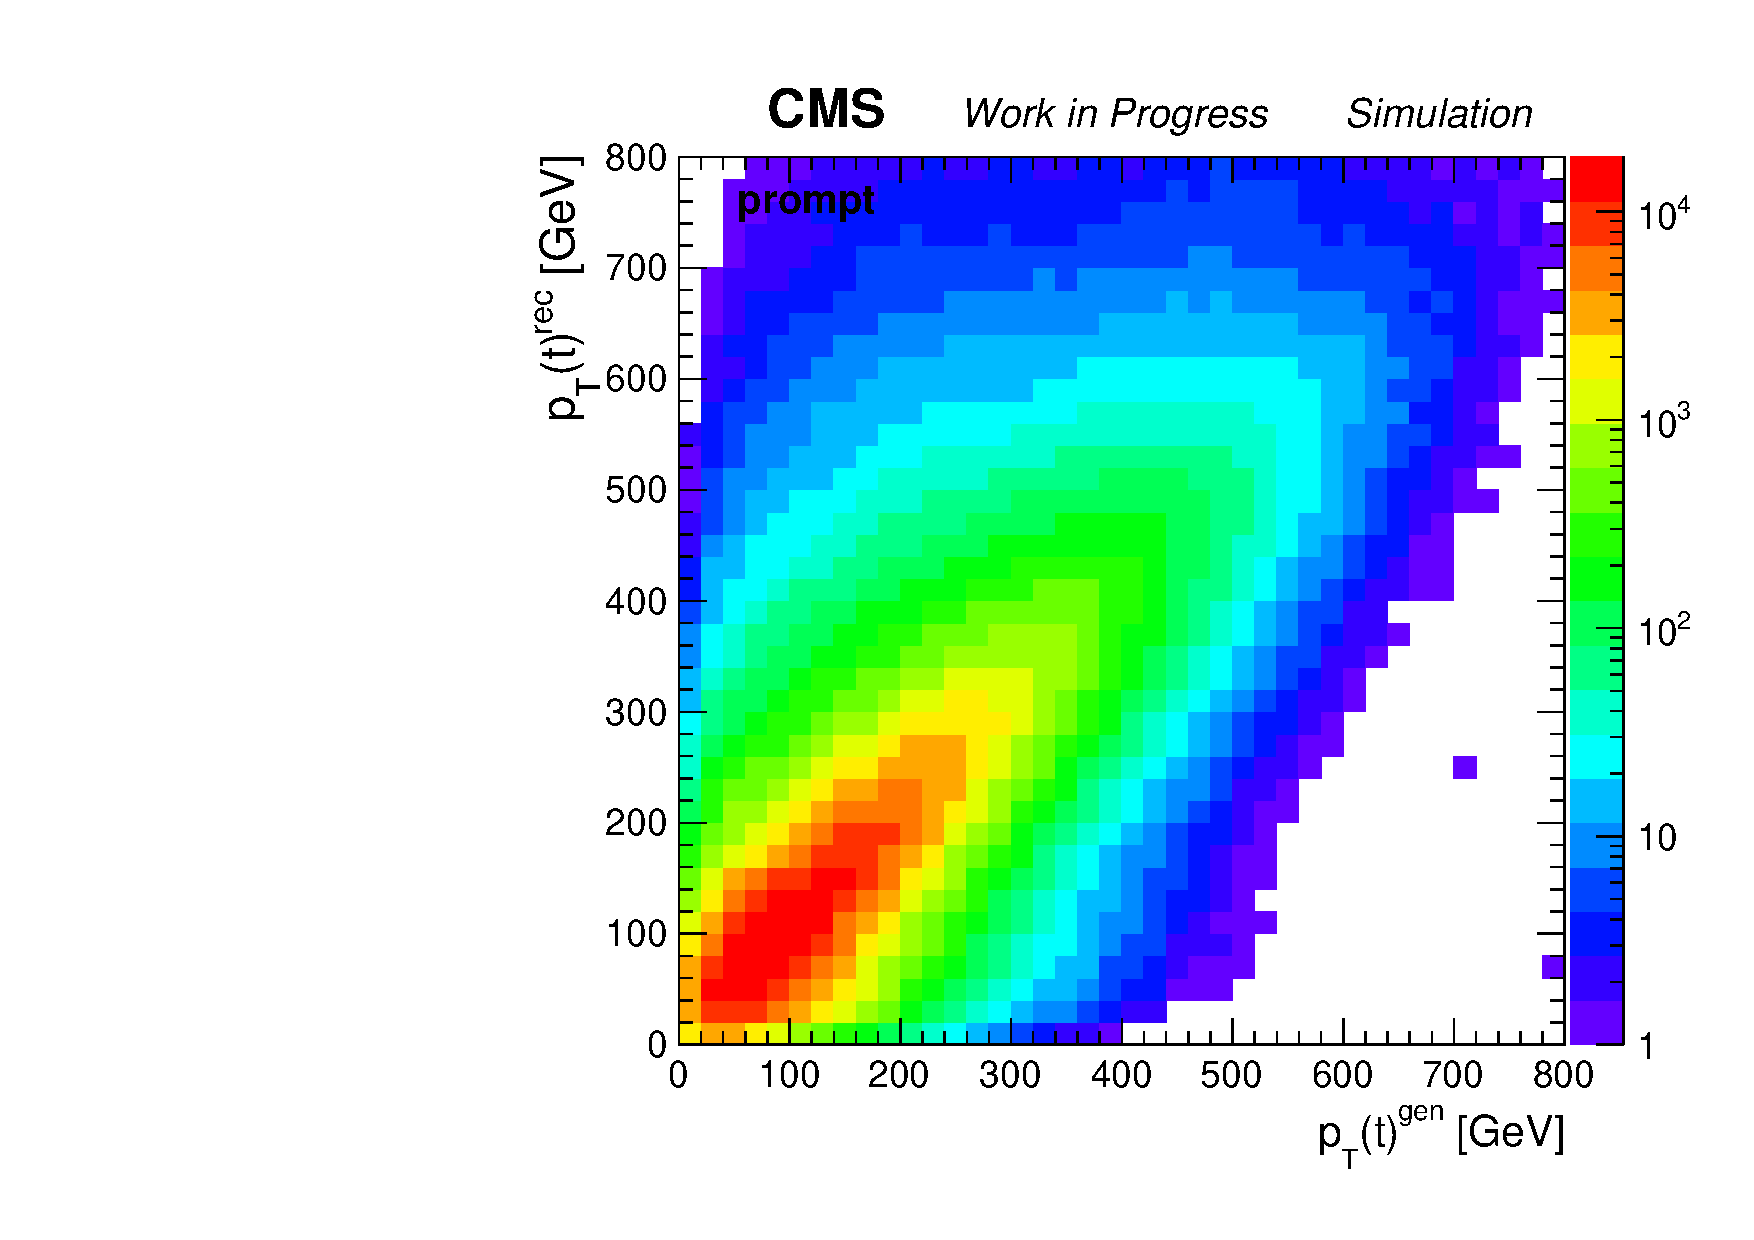
\includegraphics[width=0.30\textwidth]{fig_fullRun2UL/KinRecoResolutions/top_pT_genreco_prompt.pdf}
    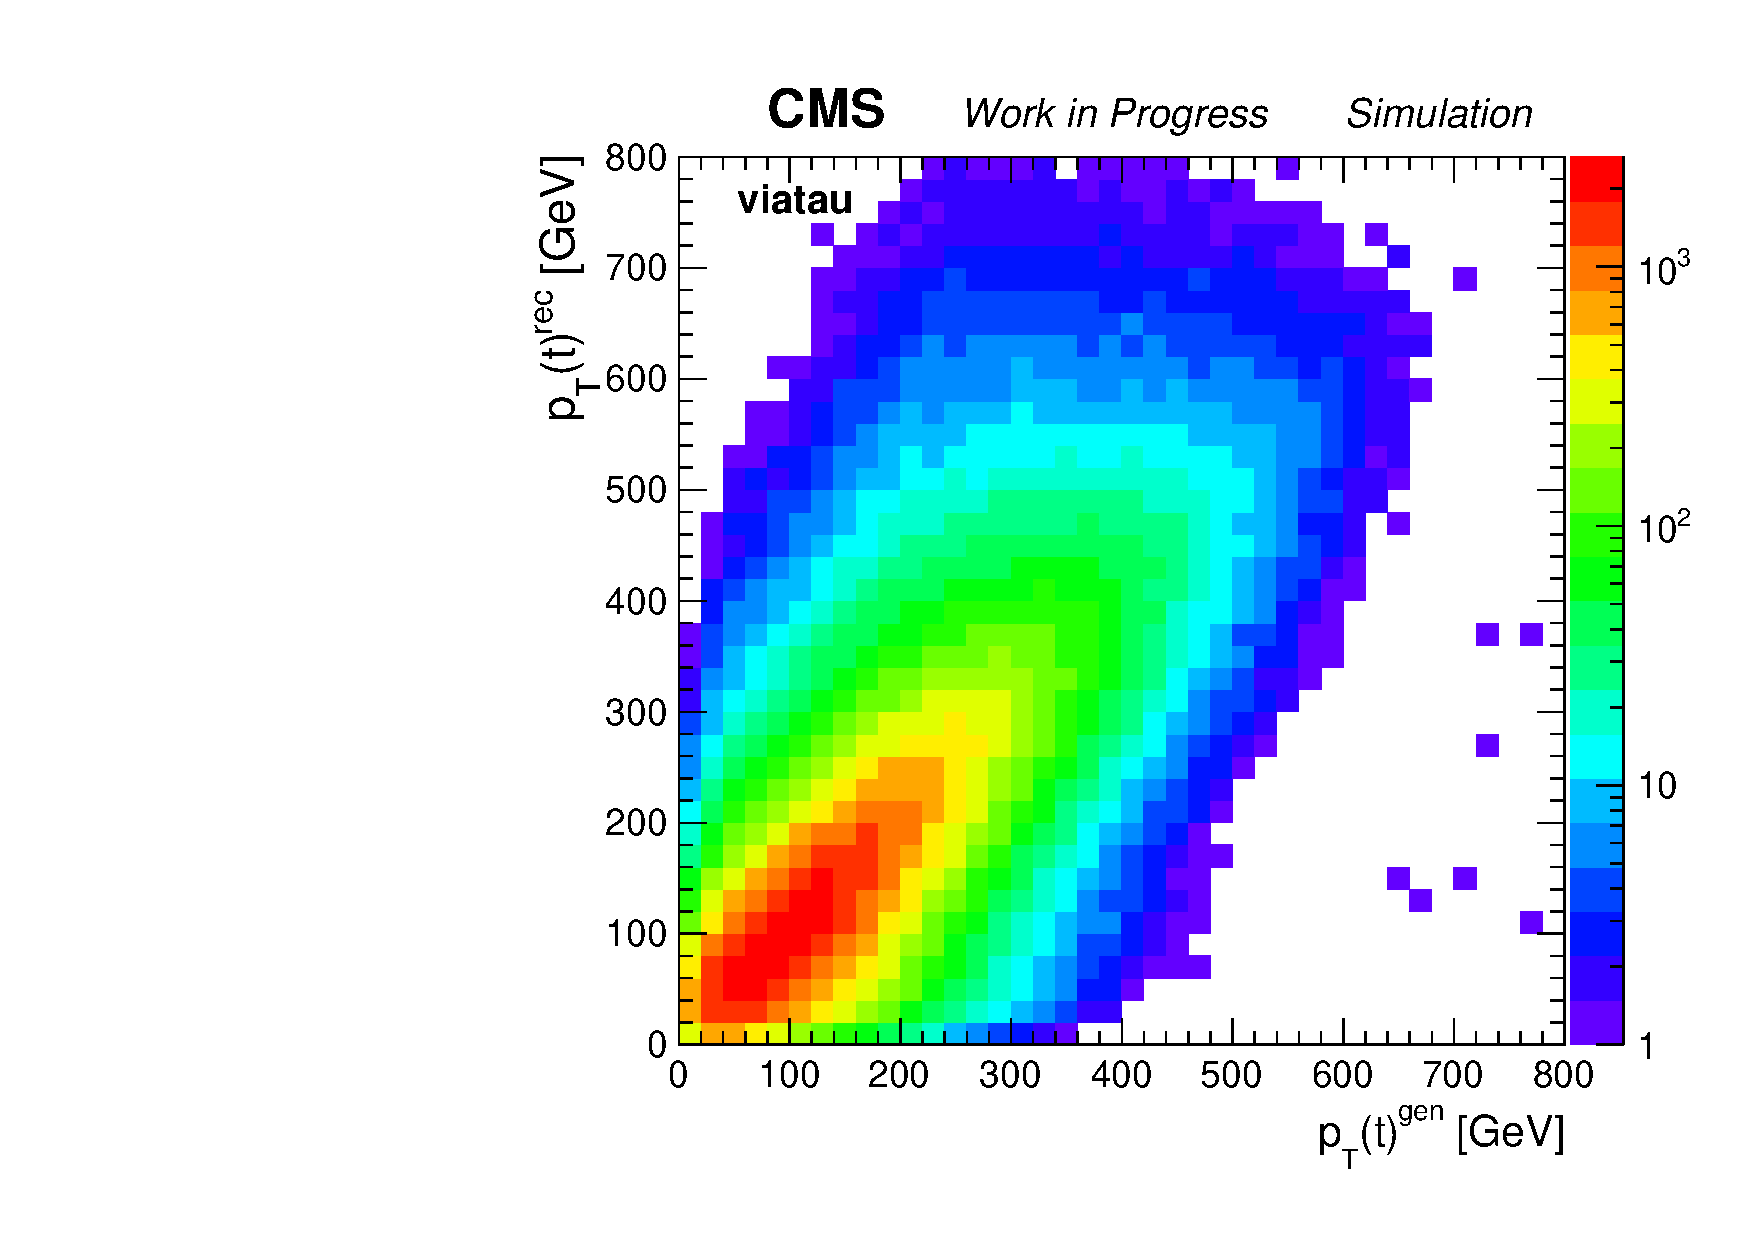
\includegraphics[width=0.30\textwidth]{fig_fullRun2UL/KinRecoResolutions/top_pT_genreco_viatau.pdf}\\
    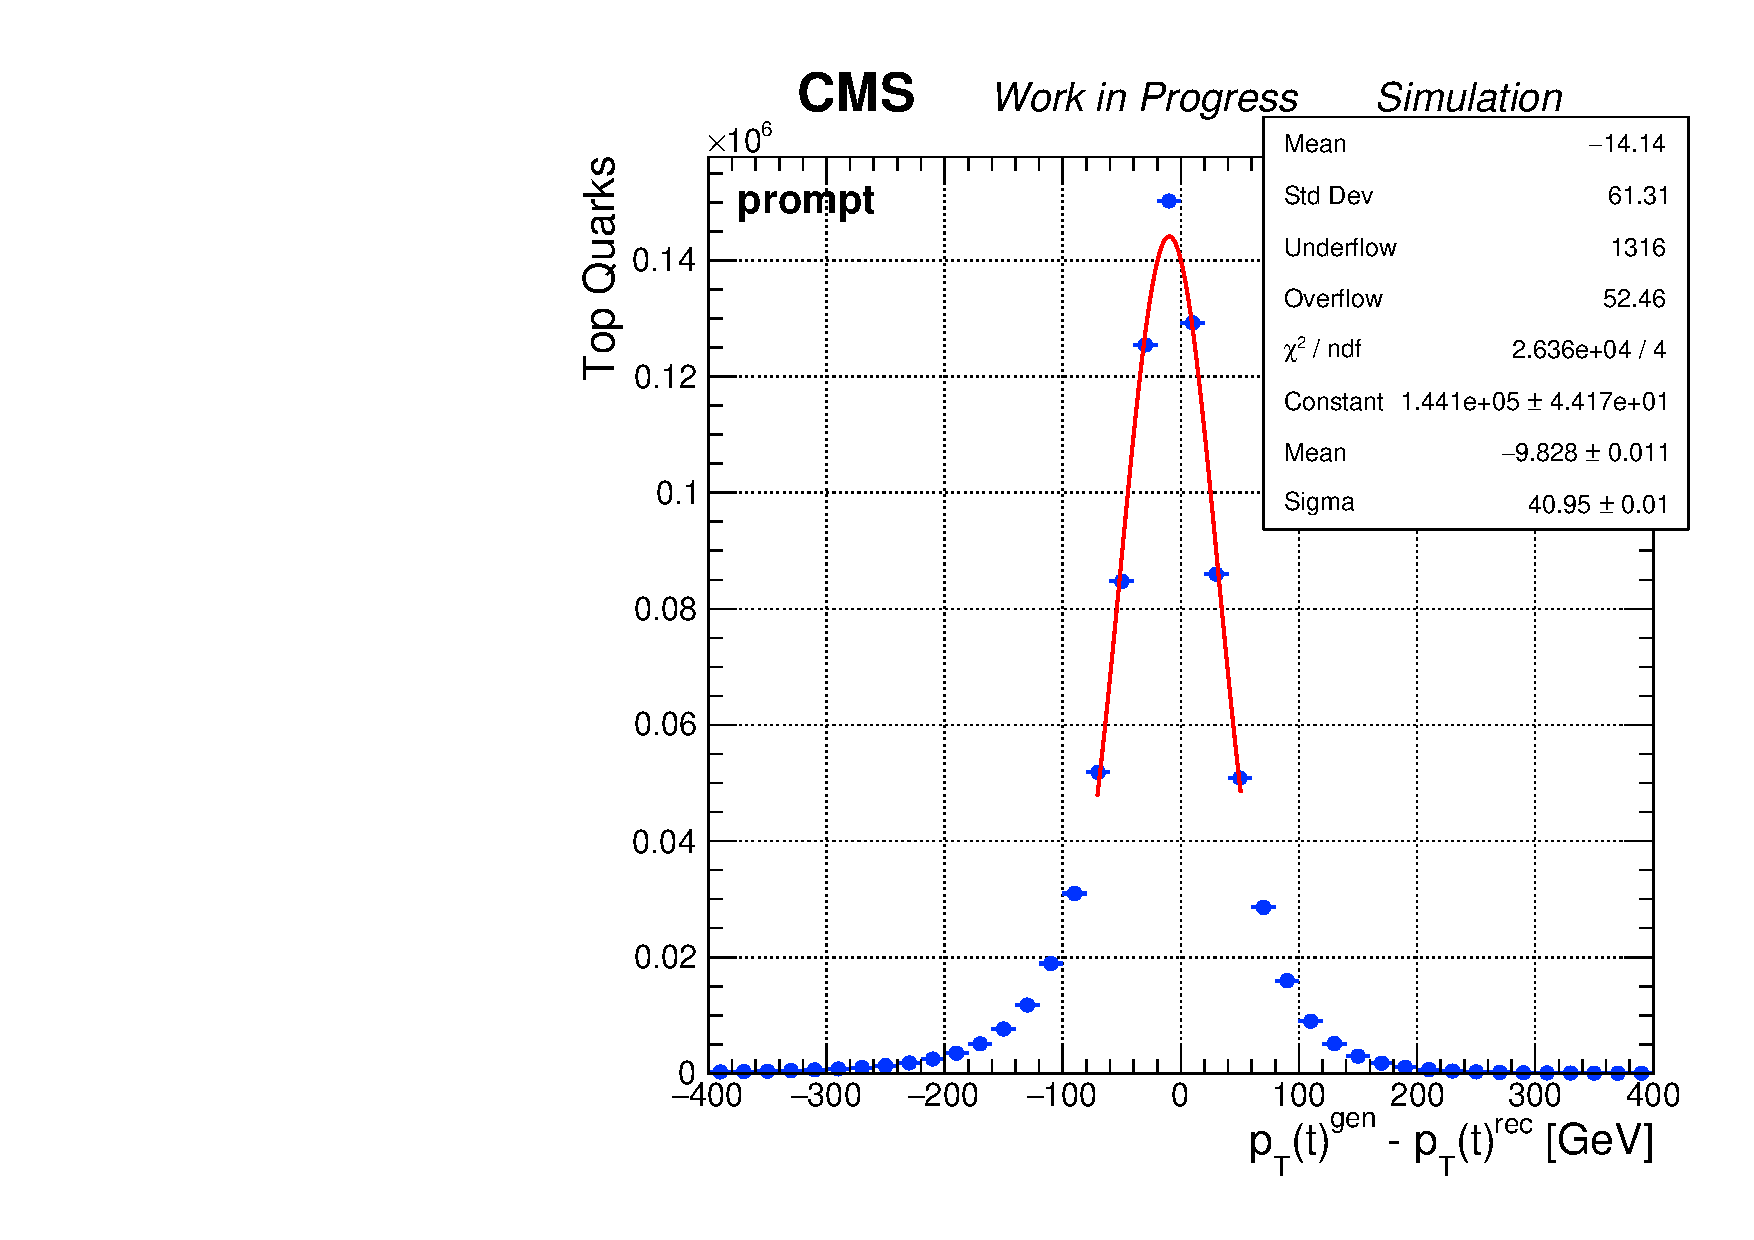
\includegraphics[width=0.30\textwidth]{fig_fullRun2UL/KinRecoResolutions/top_pT_residual_prompt.pdf}
    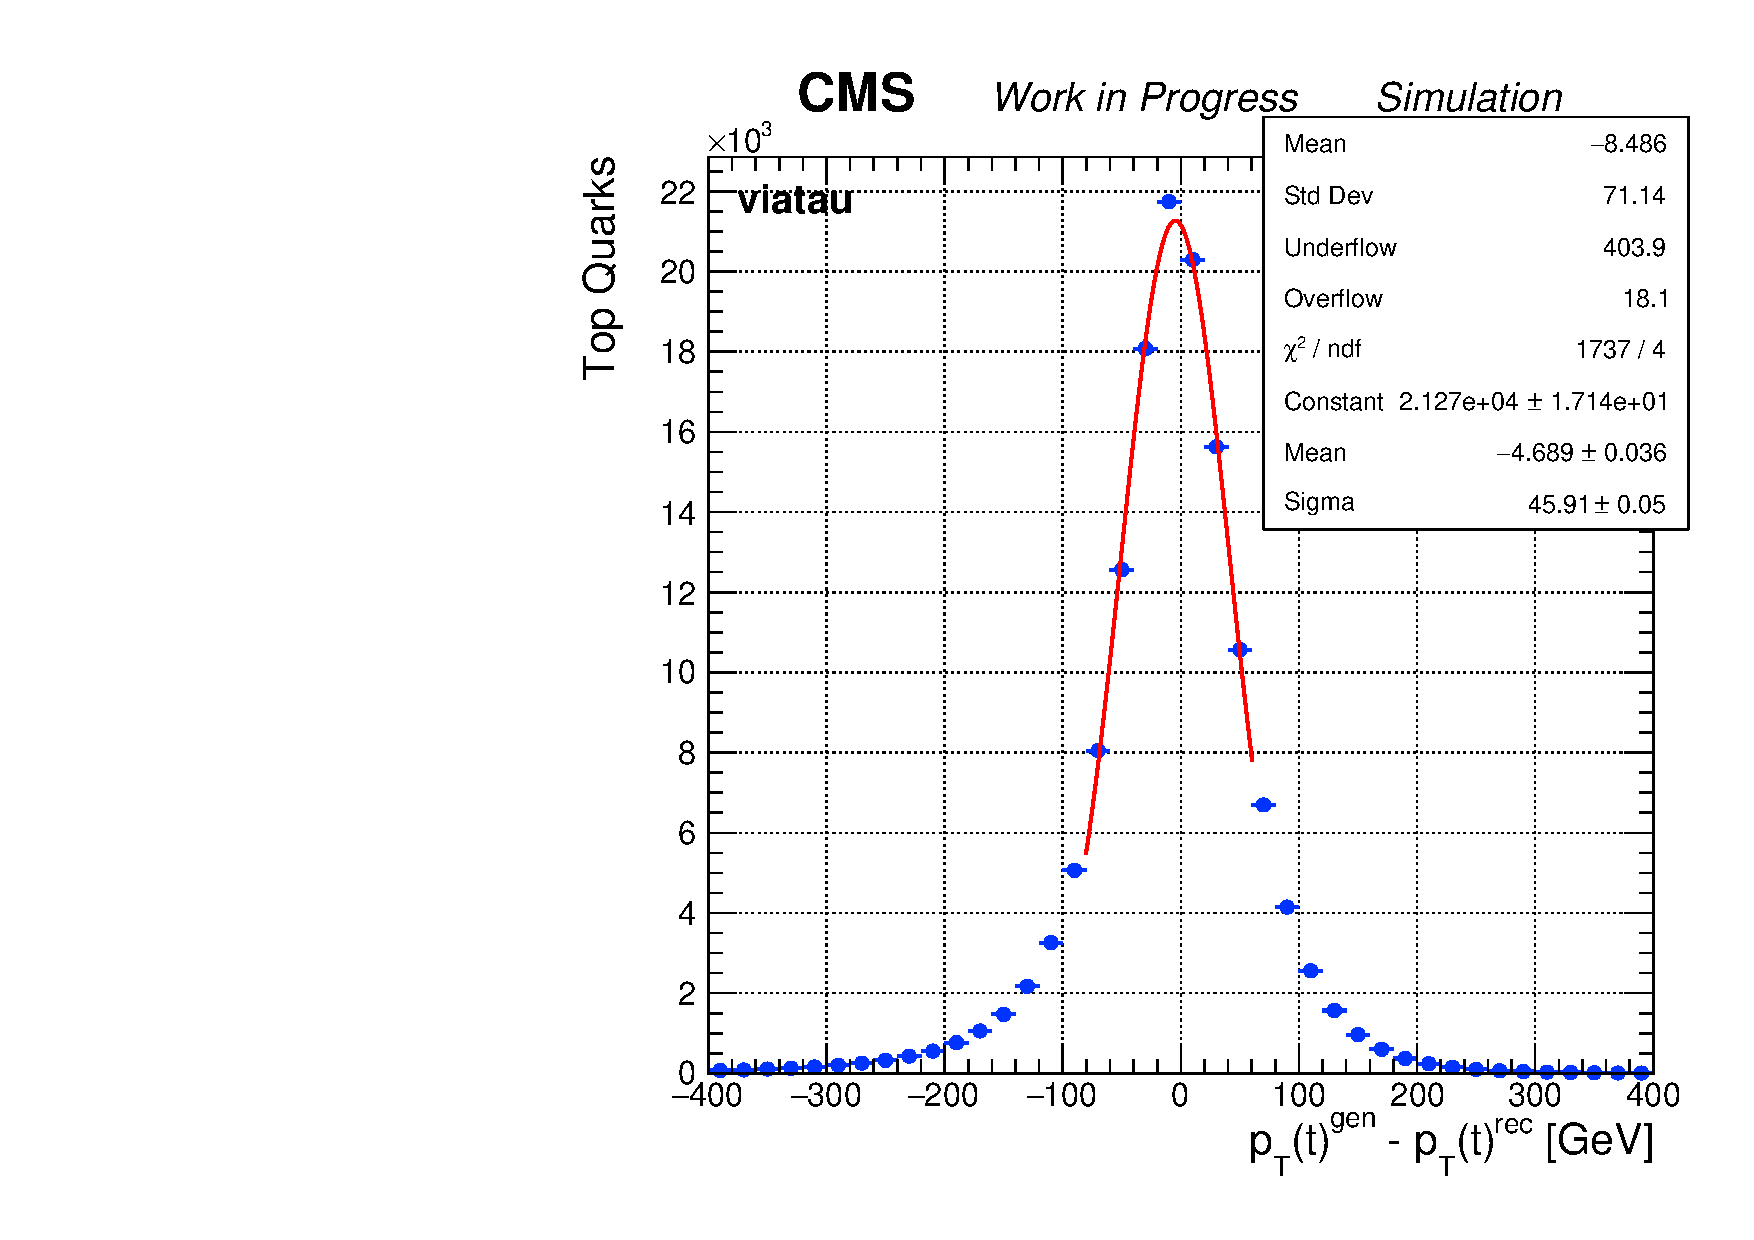
\includegraphics[width=0.30\textwidth]{fig_fullRun2UL/KinRecoResolutions/top_pT_residual_viatau.pdf}\\
    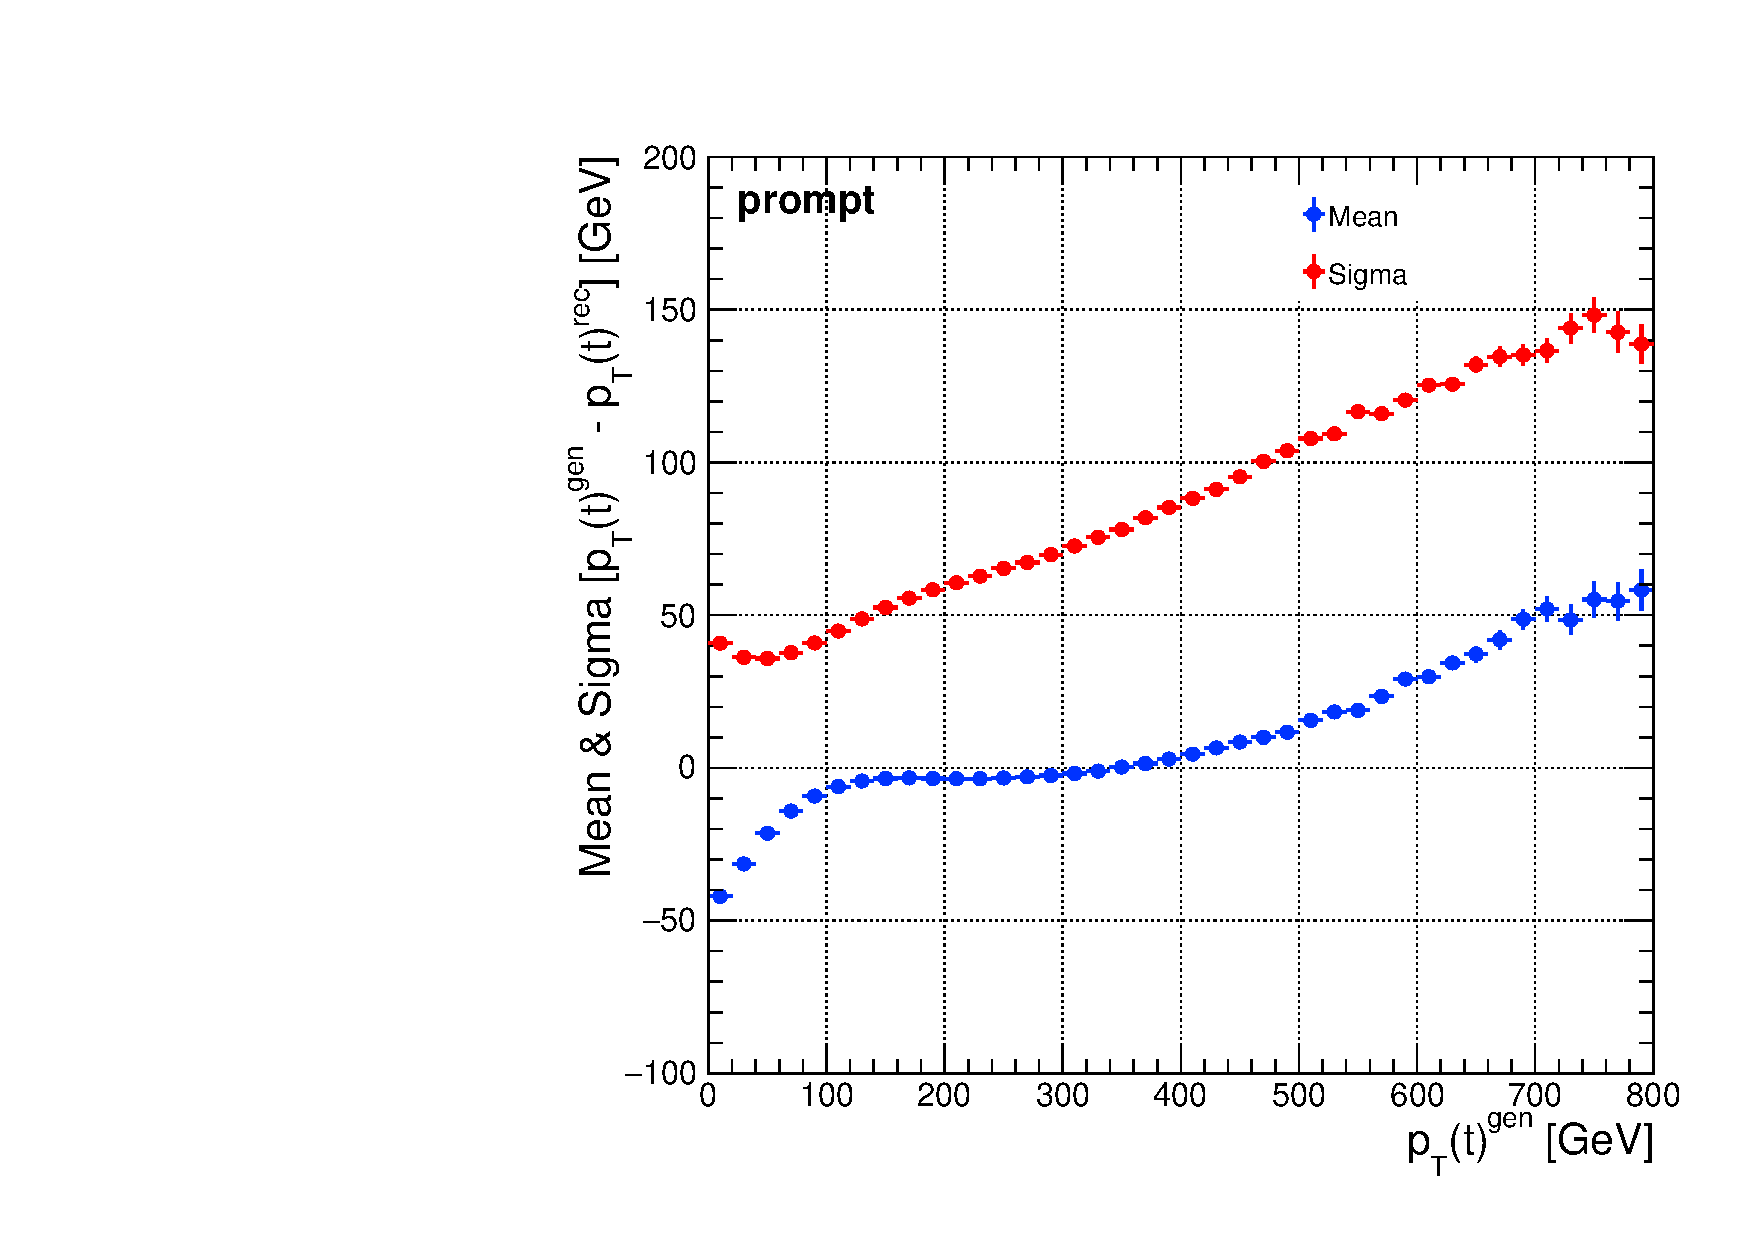
\includegraphics[width=0.30\textwidth]{fig_fullRun2UL/KinRecoResolutions/top_pT_multiresidual_prompt.pdf}
    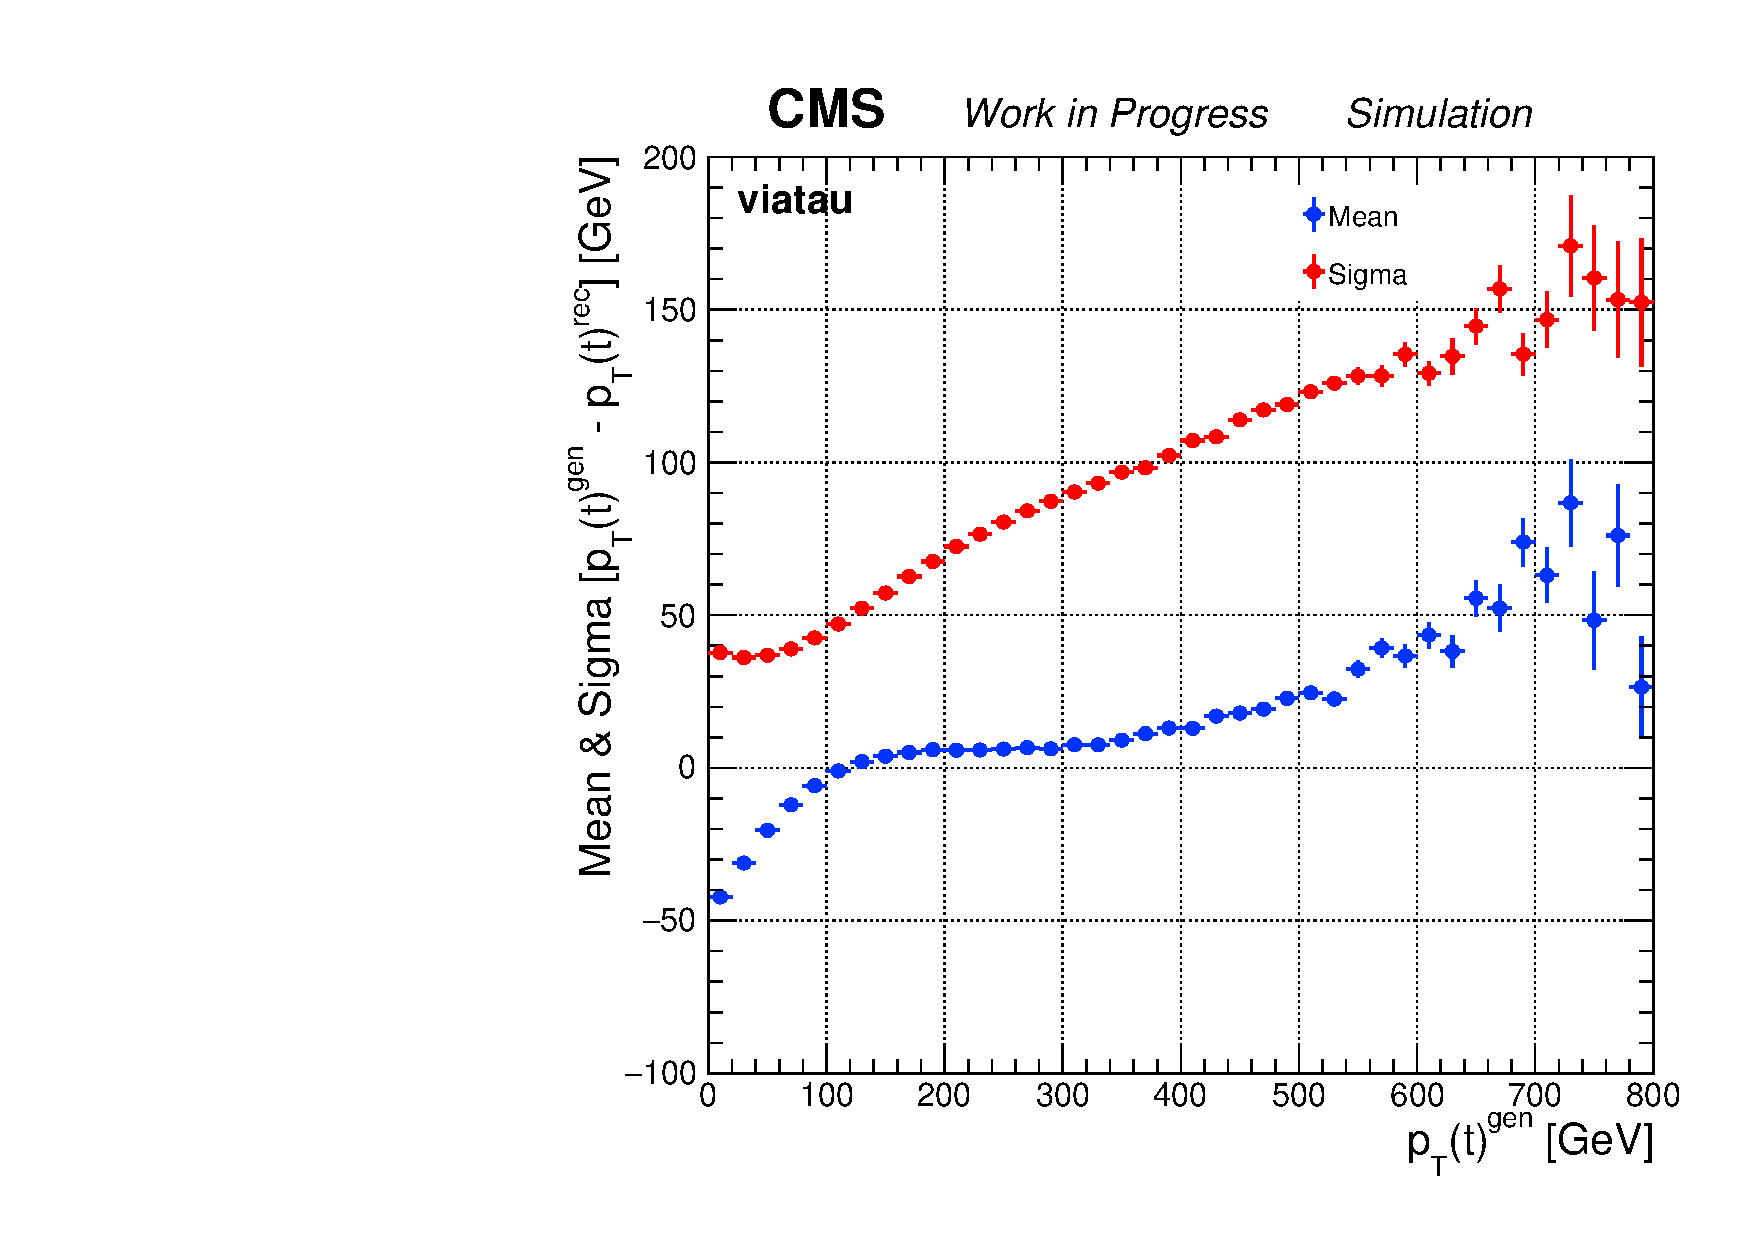
\includegraphics[width=0.30\textwidth]{fig_fullRun2UL/KinRecoResolutions/top_pT_multiresidual_viatau.pdf}\\
    \caption{\small Top: True and reconstructed \ptt\ obtained for prompt (left) and via tau (right) \ttbar dilepton events.
    Middle: The difference between true and reconstructed \ptt\ in bins of true \ptt\ (fitted with a Gaussian function for illustration).
    Bottom: The differential mean and sigma from Gaussian fits, with respect to true \ptt, of the difference between true and reconstructed \ptt\ obtained for prompt and via tau \ttbar dilepton events.
    The simulated samples are normalized to an integrated luminosity of \lumivalueRuniiUL.}
    \label{fig:kinrec:resolution-ptt}
 \end{center}
\end{figure}

\begin{figure}
  \begin{center}
    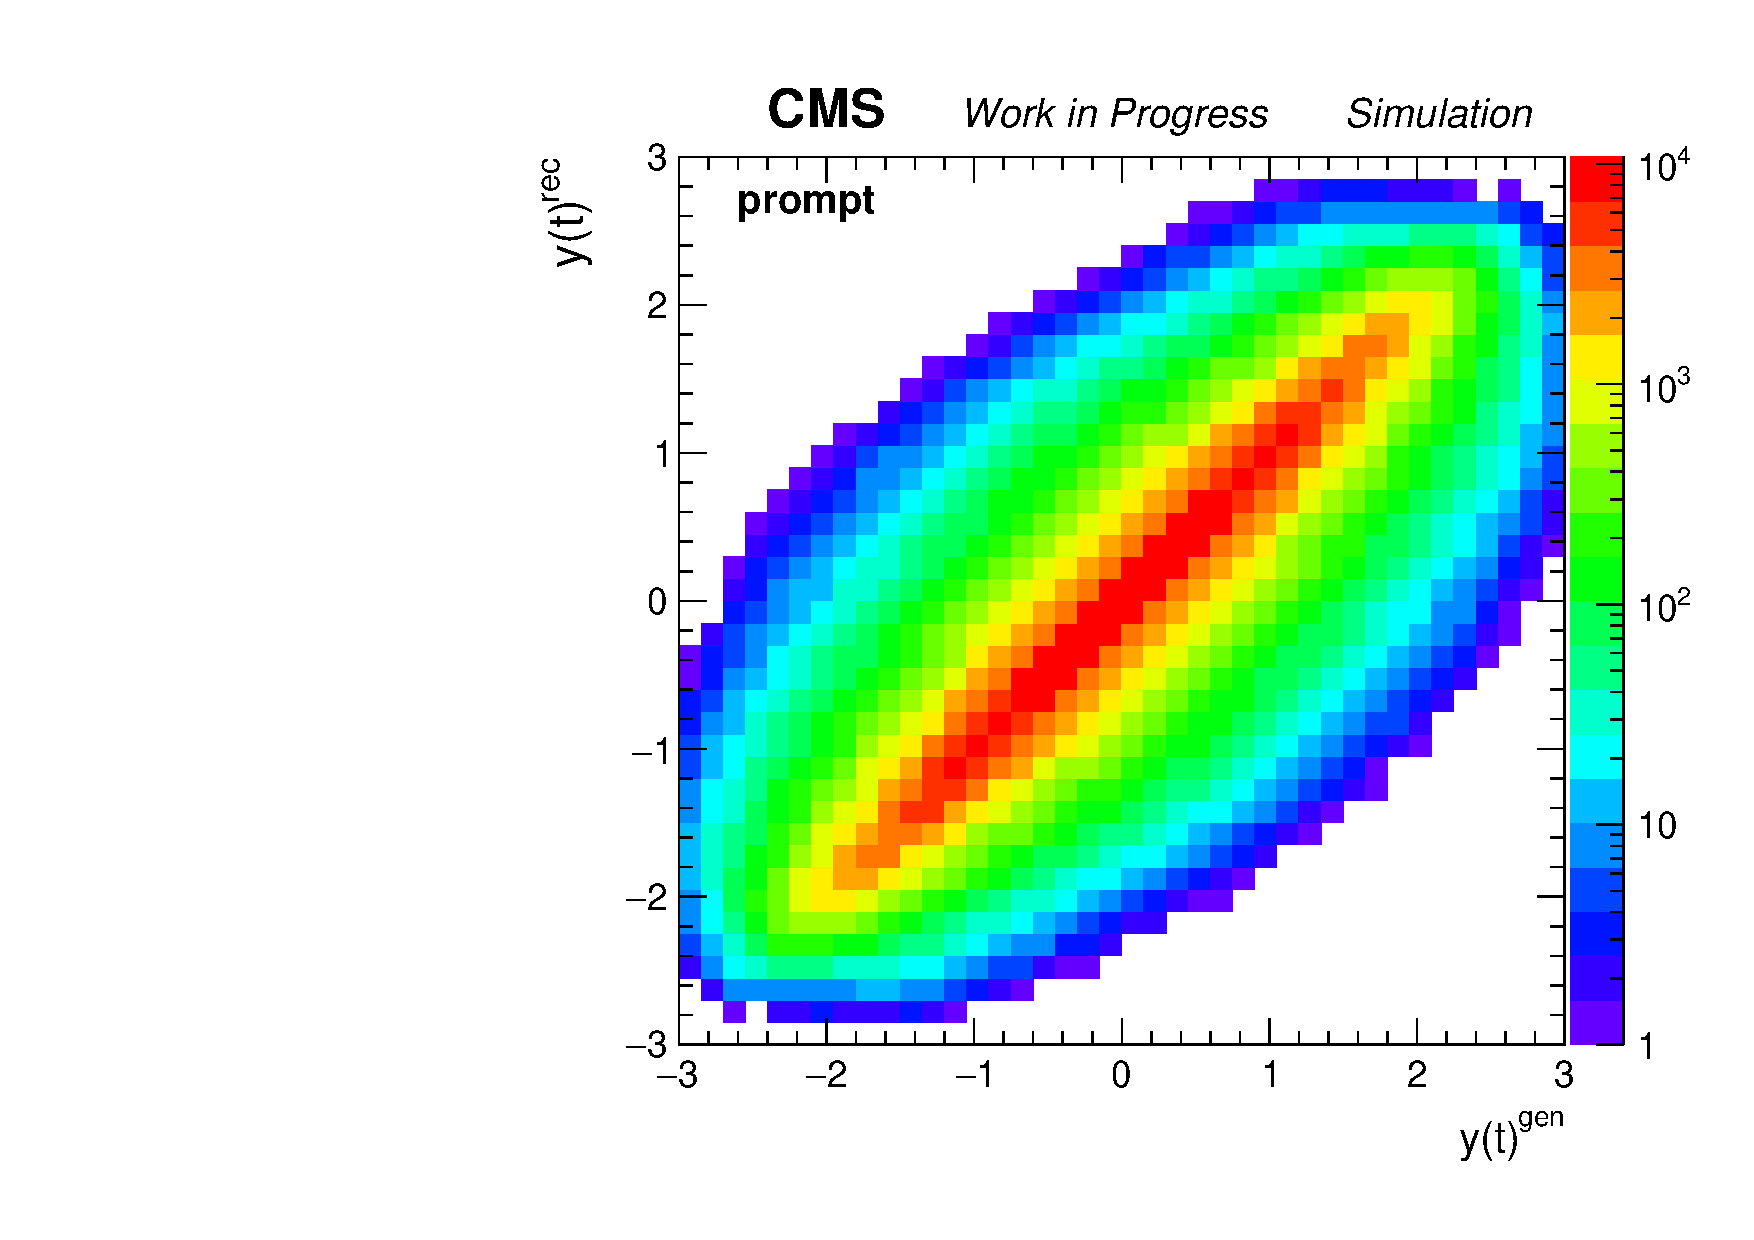
\includegraphics[width=0.30\textwidth]{fig_fullRun2UL/KinRecoResolutions/top_rapidity_genreco_prompt.pdf}
    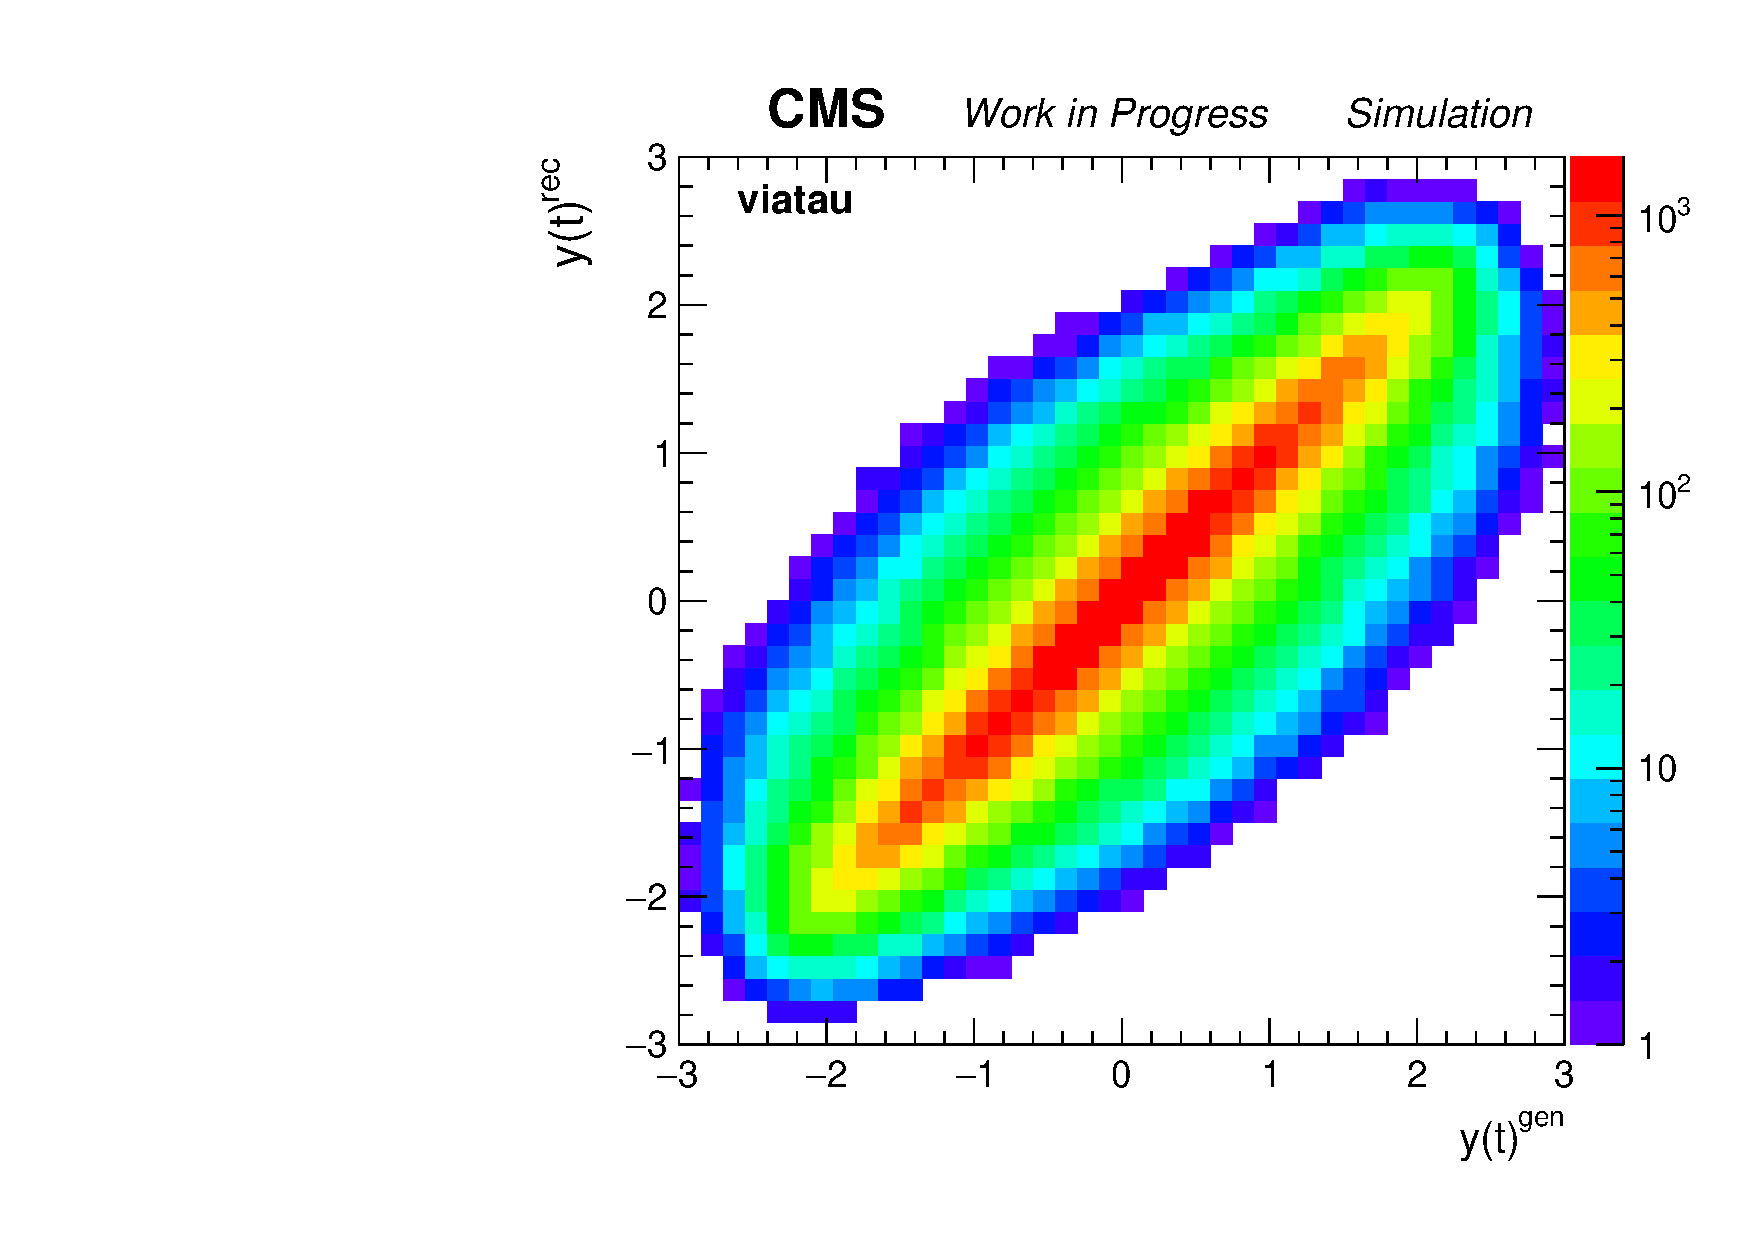
\includegraphics[width=0.30\textwidth]{fig_fullRun2UL/KinRecoResolutions/top_rapidity_genreco_viatau.pdf}\\
    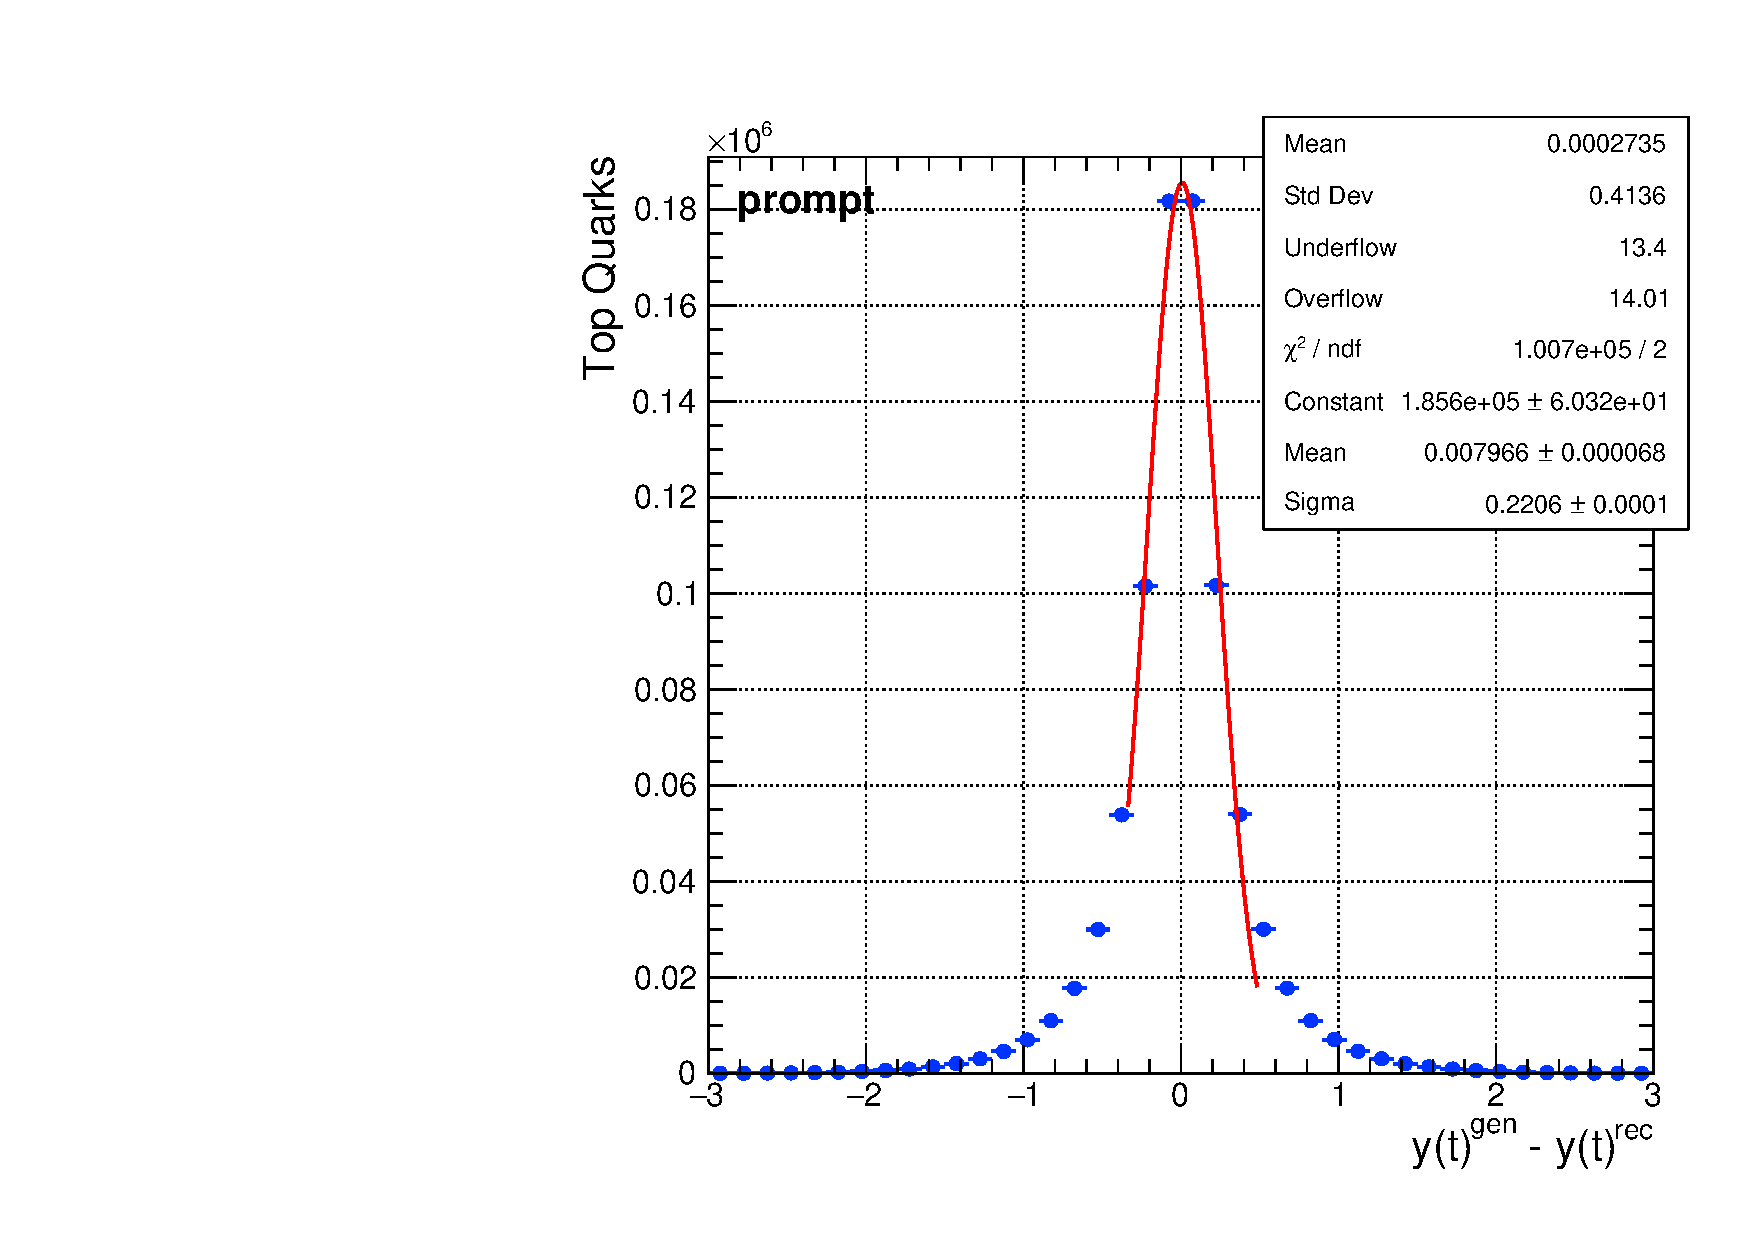
\includegraphics[width=0.30\textwidth]{fig_fullRun2UL/KinRecoResolutions/top_rapidity_residual_prompt.pdf}
    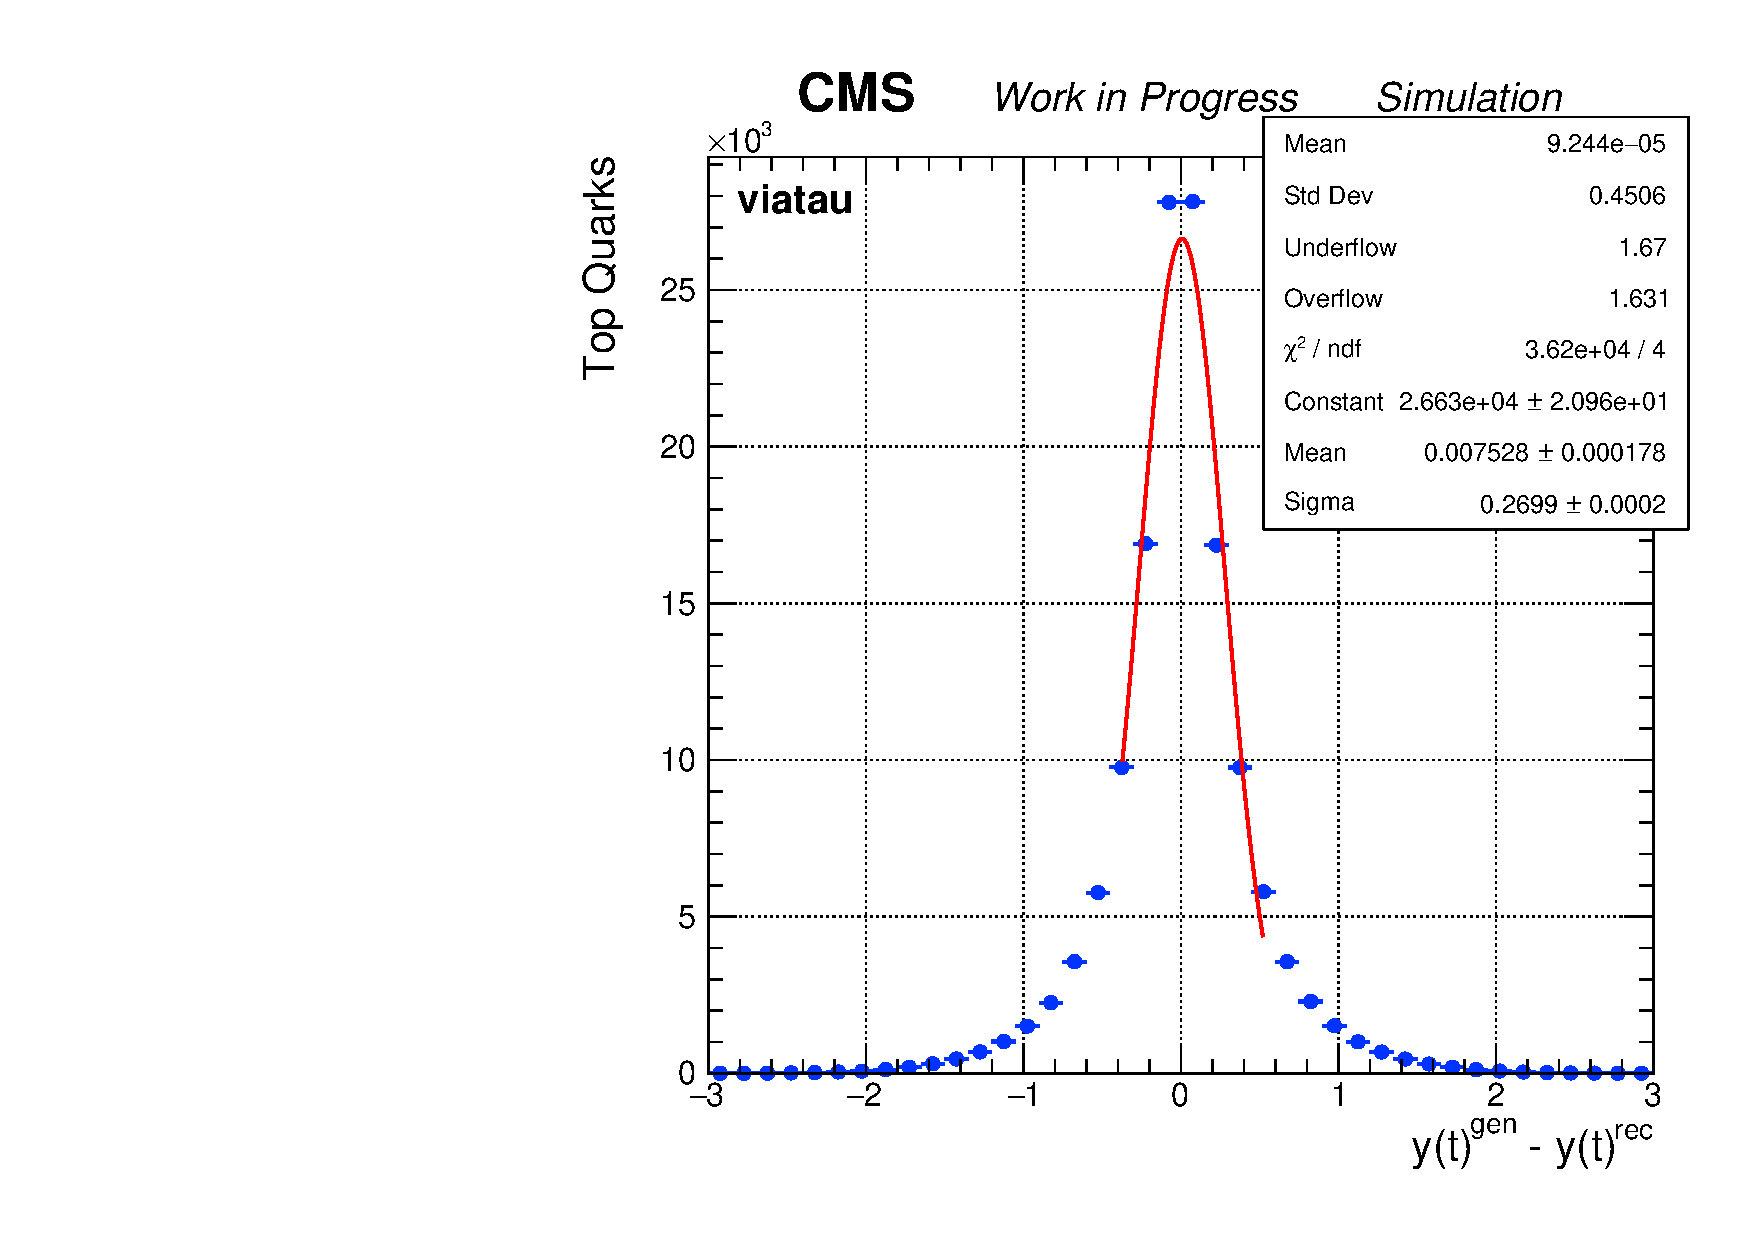
\includegraphics[width=0.30\textwidth]{fig_fullRun2UL/KinRecoResolutions/top_rapidity_residual_viatau.pdf}\\
    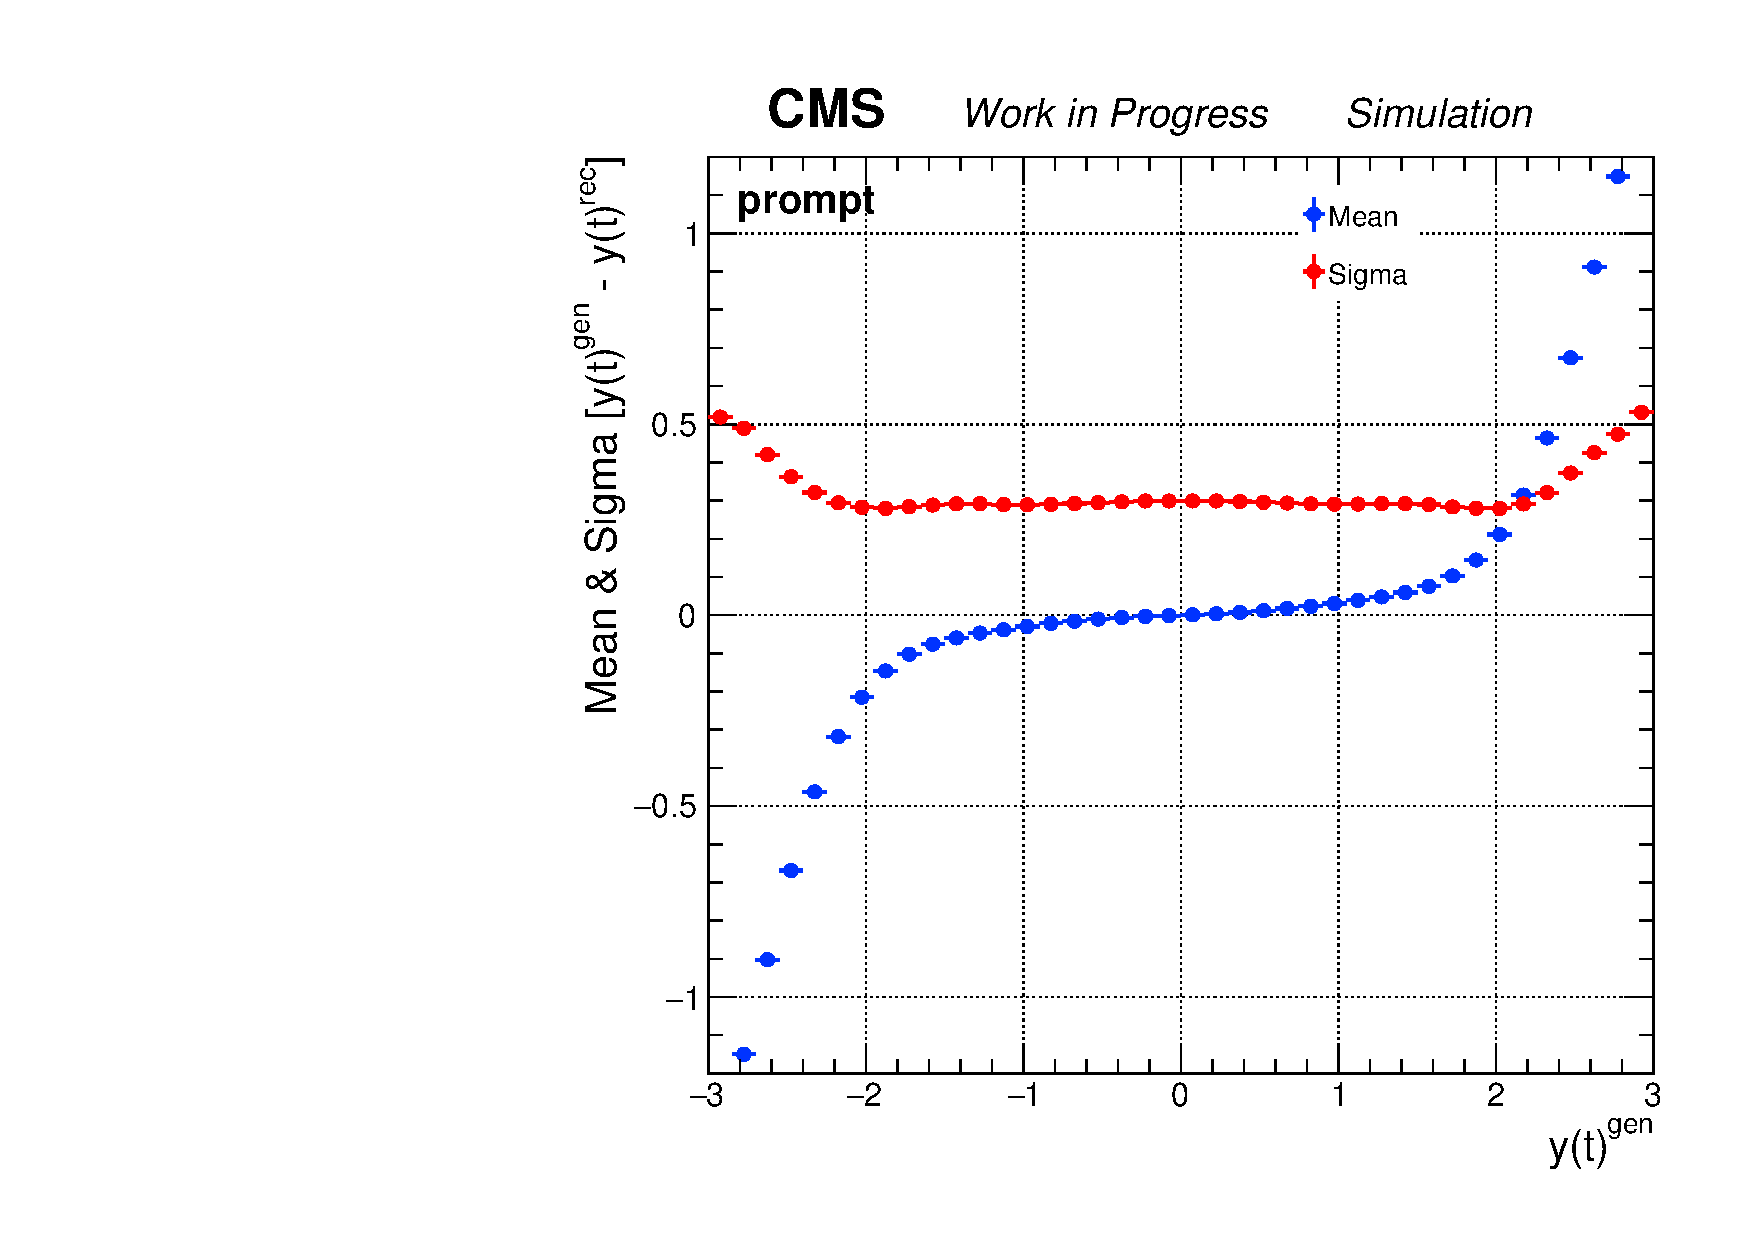
\includegraphics[width=0.30\textwidth]{fig_fullRun2UL/KinRecoResolutions/top_rapidity_multiresidual_prompt.pdf}
    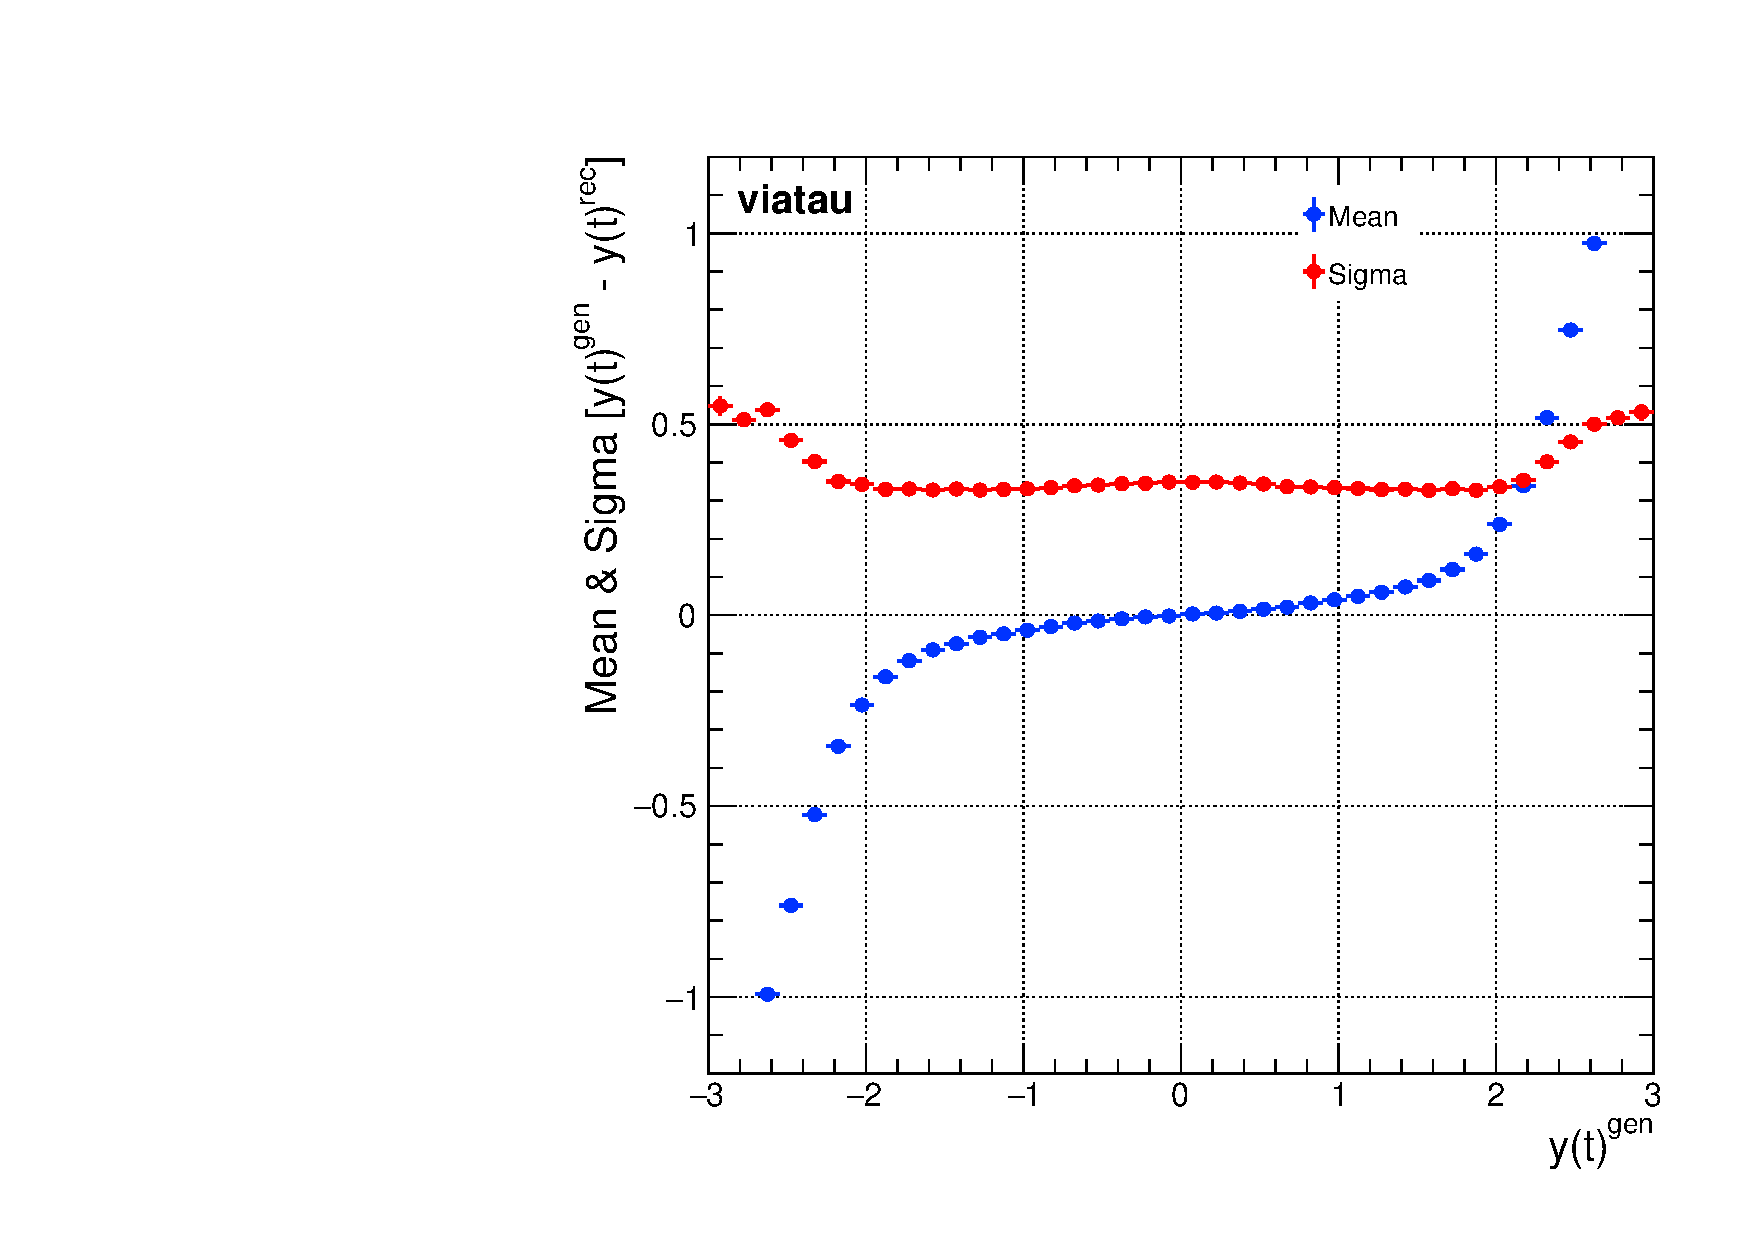
\includegraphics[width=0.30\textwidth]{fig_fullRun2UL/KinRecoResolutions/top_rapidity_multiresidual_viatau.pdf}\\
    \caption{\small Top: True and reconstructed \yt\ obtained for prompt (left) and via tau (right) \ttbar dilepton events.
    Middle: The difference between true and reconstructed \yt\ in bins of true \yt\ (fitted with a Gaussian function for illustration).
    Bottom: The differential mean and sigma from Gaussian fits, with respect to true \yt, of the difference between true and reconstructed \yt\ obtained for prompt and via tau \ttbar dilepton events.
    The simulated samples are normalized to an integrated luminosity of \lumivalueRuniiUL.}
    \label{fig:kinrec:resolution-yt}
 \end{center}
\end{figure}


\section{\ensuremath{\mathrm{Z+Jets}} Background Determination}
The expected background contributions from \ttbar, $tW$, \wjets, and diboson processes are directly taken from the MC simulations.
The \zjets\ background contribution in the selected phase space is not modeled accurately in MC simulations, and the normalization of the \zjets\ background contribution corrected using global normalization scale factors, which are determined from a binned template fit to the data using TFractionFitter as described in~\cite{CMS-PAS-TOP-20-006}\cite{BARLOW1993219}.
TFractionFitter is a class in the ROOT~\cite{Antcheva:2011zz} data analysis framework that performs a simultaneous binned Poisson maximum likelihood fit of multiple MC templates in order to determine the linear combination of templates and fractions that best describe the recorded data. 
Within the vetoed $Z$ boson mass peak control region $\SI{76}{\GeV} < \mll < \SI{106}{\GeV}$, MC templates obtained from the MC simulated samples for \zjets\ processes $\text{T}_{\zjets}$ and the sum of all other MC contributions $\text{T}_\text{Other}$ are fitted to the \mll distributions in the data template $\text{T}_\text{Data}$ as:
\begin{linenomath*}
\begin{align}
\text{T}_\text{Data} = f_{\zjets} \cdot \text{T}_{\zjets} + f_{\text{Other}} \cdot \text{T}_\text{Other}
\end{align}
\end{linenomath*}
where $f_{\zjets}$ and $f_{\text{Other}}$ are the fractions obtained from the fit.
Separate global normalization scale factors ($\mathcal{SF}$) are fitted in the \ee and \mumu channels:
\begin{linenomath*}
\begin{align}
\mathcal{SF}_{ee} &= \frac{f_{\zjets}^{\ee} \cdot \mathcal{N}_\text{Data}^{\ee}}{\mathcal{N}_{\zjets}^{\ee}} \\
\mathcal{SF}_{\mu\mu} &= \frac{f_{\zjets}^{\mumu} \cdot \mathcal{N}_\text{Data}^{\mumu}}{\mathcal{N}_{\zjets}^{\mumu}}
\end{align}
\end{linenomath*}
where $\mathcal{N}_{\zjets}$ and $\mathcal{N}_\text{Data}$ are the number of events in the \zjets\ template and data distribution.
The \emu and combined channel scale factors are calculated as:
\begin{linenomath*}
\begin{gather}
\mathcal{SF}_{\emu} = \sqrt{\mathcal{SF}_{\ee} \times \mathcal{SF}_{\mumu}} \\
\mathcal{SF}_{\ell \bar{\ell}} = \frac{\mathcal{SF}_{\ee} \cdot \mathcal{N}_\text{Data}^{\ee} + \mathcal{SF}_{\mumu} \cdot \mathcal{N}_\text{Data}^{\mumu} + \mathcal{SF}_{\emu} \cdot \mathcal{N}_\text{Data}^{\emu}}{\mathcal{N}_\text{Data}^{\ee} + \mathcal{N}_\text{Data}^{\mumu} + \mathcal{N}_\text{Data}^{\emu}}.
\end{gather}
\end{linenomath*}
To enhance \zjets\ statistics in the orthogonal phase space of the $Z$ boson mass peak control region, \MET and b-tagging event selection requirements are omitted, as is the requirement of a kinematic reconstruction solution.
The fits performed by TFractionFitter of the two MC templates to the data template within the $Z$ boson mass peak control region are shown for Full Run II in figure~\ref{fig:fitstatusfullRun2UL}
The resulting \zjets\ global normalization scale factors are shown in table~\ref{tab:dysffullRun2UL}.

\begin{figure}[!htb]
  \begin{center}
        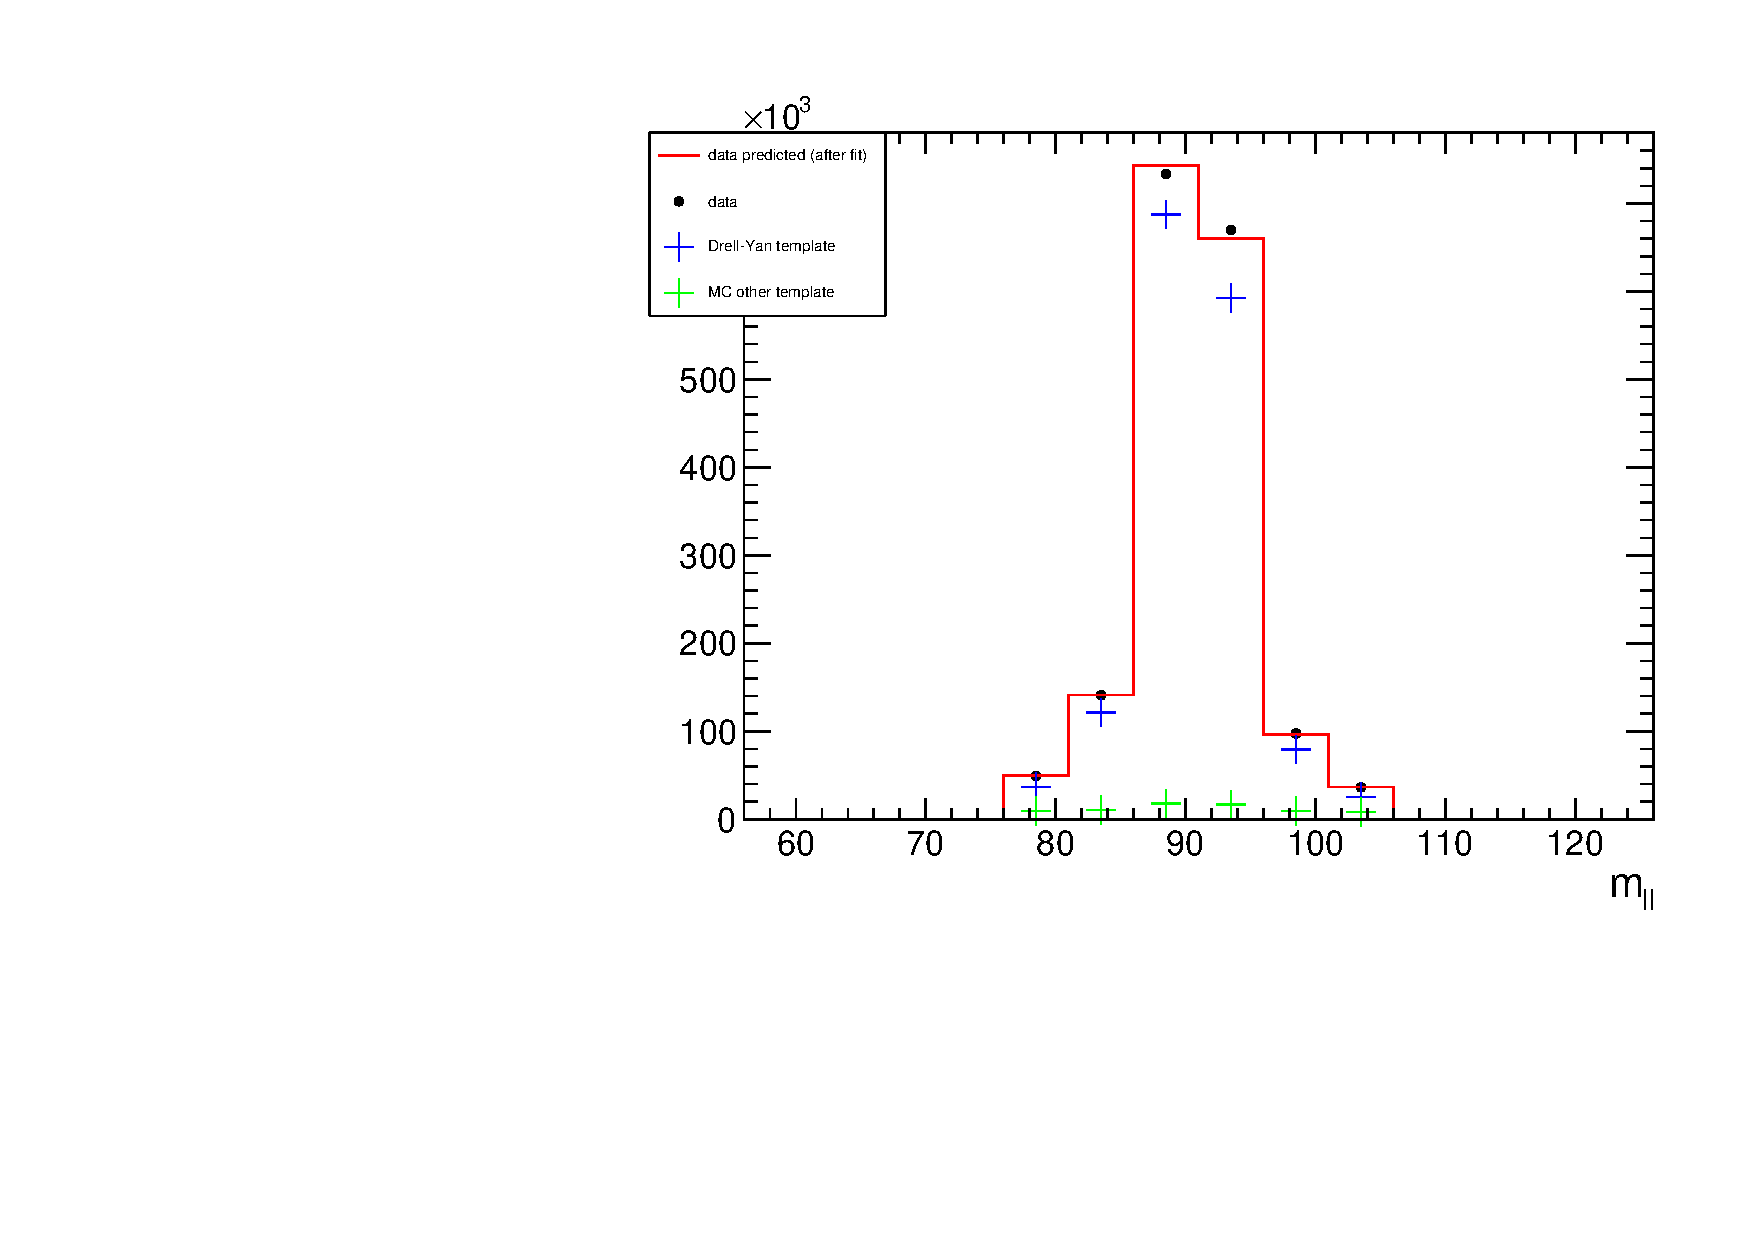
\includegraphics[width=0.30\textwidth]{fig_fullRun2UL/fit_status_ee.pdf}
        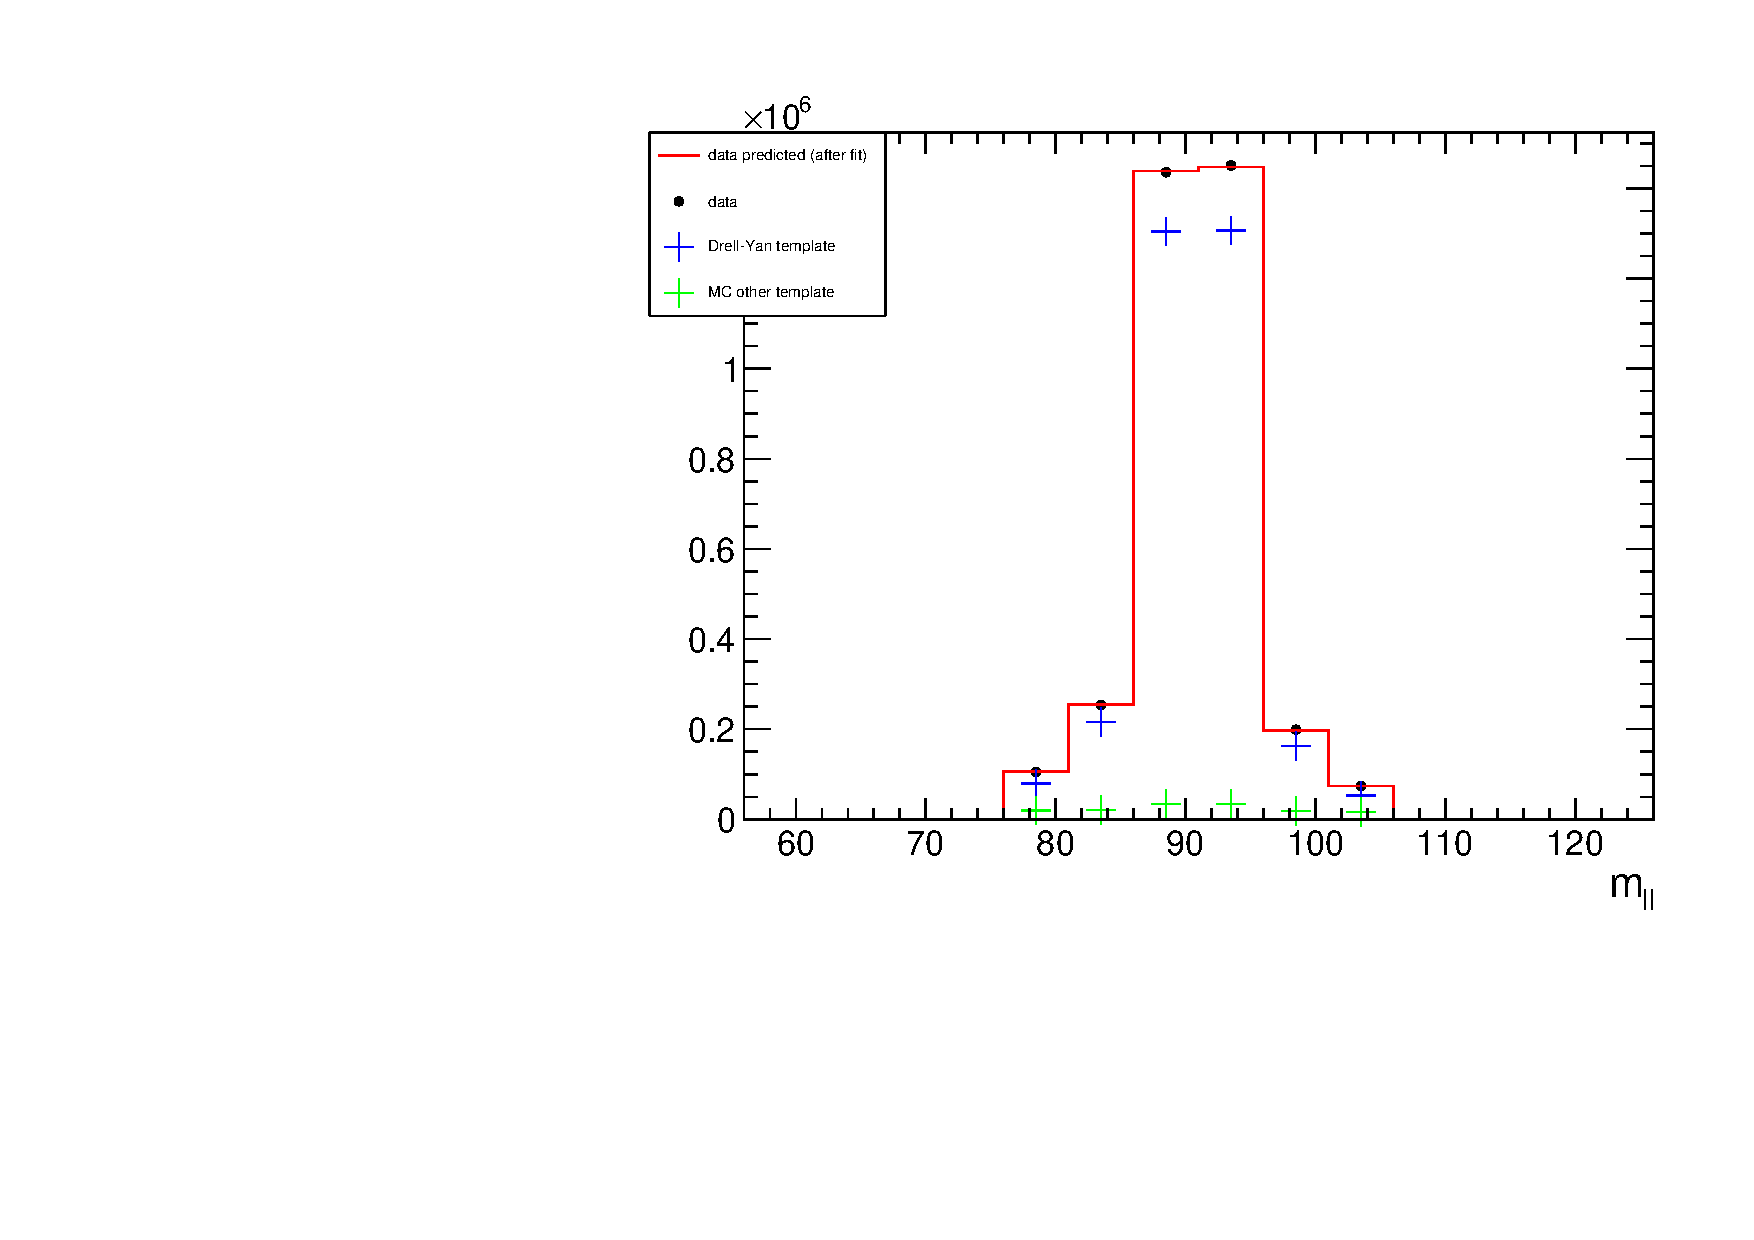
\includegraphics[width=0.30\textwidth]{fig_fullRun2UL/fit_status_mumu.pdf}
        \caption{
            \small Dilepton mass distributions in the $Z$ boson mass peak control between $\SI{76}{\GeV} < \mll < \SI{106}{\GeV}$ are shown for the \ee (left) and \mumu (right) channels for Full Run II. 
            The data template $\text{T}_\text{Data}$ is illustrated by black dots, the \zjets\ template $\text{T}_{\zjets}$ is shown in blue, and the sum of all other MC contributions template $\text{T}_\text{Other}$ is green. 
            The red histogram shows the result of the fit performed by TFractionFitter.
            \label{fig:fitstatusfullRun2UL}
    }
  \end{center}
\end{figure}

\begin{table}[!htb]
 \begin{center}
    \begin{tabular}{|c|cccc|}
      \hline 
      \multicolumn{5}{|c|}{\zjets\ Global Normalization Scale Factors} \\
      \hline 
                 & $\mathcal{SF}_{\ee}$ & $\mathcal{SF}_{\mumu}$ & $\mathcal{SF}_{\emu}$ & $\mathcal{SF}_{\ell \bar{\ell}}$ \\
      \hline
      2016preVFP & $1.081 \pm 0.005$ & $1.071 \pm 0.004$ & $1.076 \pm 0.013$ & $1.074 \pm 0.019$ \\
      2016postVFP & $1.112 \pm 0.006$ & $1.144 \pm 0.004$ & $1.128 \pm 0.015$ & $1.133 \pm 0.021$ \\
      2017 & $1.078 \pm 0.004$ & $1.103 \pm 0.002$ & $1.091 \pm 0.009$ & $1.095 \pm 0.012$ \\
      2018 & $1.042 \pm 0.003$ & $1.047 \pm 0.002$ & $1.044 \pm 0.007$ & $1.045 \pm 0.01$ \\
      Full Run II  & $1.067 \pm 0.002$ & $1.079 \pm 0.001$ & $1.073 \pm 0.005$ & $1.075 \pm 0.007$ \\
      \hline
    \end{tabular}
  \caption{Data-driven \zjets\ global normalization scale factors $\pm$ the statistical uncertainty from the fit, determined within the vetoed $Z$ boson mass peak control region $\SI{76}{\GeV} < \mll < \SI{106}{\GeV}$ using TFractionFitter.}
  \label{tab:dysffullRun2UL}     
 \end{center}
\end{table}


\section{Event Yields}
The eight consecutive event selection steps are summarized as:
\begin{itemize}
    \item {\bf MET Filters:} Events that are not excluded due to MET filters ({\bf 1a}),
    \item {\bf Triggers:} Events that pass trigger requirements ({\bf 1b}),
    \item {\bf Primary Vertex:} Events with primary vertex passing selection requirements ({\bf 1}),
    \item {\bf Leptons:} Events with exactly two oppositely-charged isolated leptons ({\bf 2}) and $m_{\ell\ell} > \SI{20}{\GeV}$ ({\bf 3}).  
            In the \mumu and \ee channels, the \zjets\ background is removed by rejecting events in the Z boson mass region $\SI{76}{\GeV} < m^{\ell\bar{\ell}} < \SI{106}{\GeV}$ ({\bf 4}),
    \item {\bf Jets:} Events with at least two jets fulfilling the jet \pT and $\eta$ requirements ({\bf 5}),
    \item {\bf Missing Transverse Energy:} Events in the \mumu and \ee channels with $\ETmiss > \SI{40}{\GeV}$ ({\bf 6}),
    \item {\bf b-Tagging:} Events include at least one b-tagged jet ({\bf 7}),
    \item {\bf Top Pair Reconstruction:} Events with at least one physically meaningful solution for the full kinematic reconstruction of a \ttbar\ system ({\bf 8}).
\end{itemize}
The numbers of observed events in the data compared to the expected events from MC simulation for Full Run II are given in Table~\ref{t-cutflowfullRun2UL} after each of the consecutive selection steps.

\begin{table}[!htb]
 \begin{center}
    \caption{\small Full Run II (\lumivalueRuniiUL) expected event yields for signal and background processes, compared to the event yields in recorded data, after each step of event selection.} 
    \label{t-cutflowfullRun2UL}
      \begin{adjustbox}{scale=0.70,center}
       {\footnotesize
        \begin{tabular}{lrrrrrrr}
\hline $\boldsymbol{\mu^+\mu^-}$ & Leptons & Jets & \ETmiss & b-Tag & Kin. Reco. \\
\hline
\ttbar\ Signal &                486260.0&               342459.0&               272219.0&               241382.0&               220154.0                \\
\ttbar\ Other &         10796.4&                8293.4&         6237.5&         4266.4&         3544.3          \\
$\ttbar+Z/W$&           1326.0&         1201.9&         988.9&          850.3&          664.0           \\
Single &                49638.5&                19065.8&                15251.4&                12362.2&                8413.4          \\
Diboson &               71079.5&                6822.1&         3549.0&         475.0&          275.8           \\
W+jets &                5268.4&         589.4&          252.8&          78.9&           78.3            \\
Z+jets &                7489000.0&              404230.0&               91862.9&                14070.5&                9951.6          \\
\hline
\textbf{MC Total} &                8113370.0&              782661.0&               390362.0&               273486.0&               \textbf{243081.0}                \\
\textbf{Data} &          8060660.0&              797354.0&               405879.0&               278054.0&               \textbf{247150.0}                \\
\hline
\hline $\boldsymbol{\mu^{\pm}}\mathbf{e^{\mp}}$ & Leptons & Jets & \ETmiss & b-Tag & Kin. Reco. \\
\hline
\ttbar\ Signal &                896402.0&               633218.0&               633218.0&               562837.0&               520593.0                \\
\ttbar\ Other &         15438.4&                11944.2&                11944.2&                8448.5&         7157.5          \\
$\ttbar+Z/W$&           2174.8&         1954.3&         1954.3&         1676.3&         1382.2          \\
Single &                90803.8&                34783.6&                34783.6&                28290.6&                20105.7         \\
Diboson &               111527.0&               6568.6&         6568.6&         773.8&          475.7           \\
W+jets &                17722.3&                1904.9&         1904.9&         354.6&          248.2           \\
Z+jets &                269816.0&               17614.8&                17614.8&                2297.5&         1803.2          \\
\hline
\textbf{MC Total} &                1403880.0&              707988.0&               707988.0&               604679.0&               \textbf{551765.0}                \\
\textbf{Data} &          1441170.0&              710103.0&               710103.0&               598682.0&               \textbf{546299.0}                \\
\hline
\hline $\mathbf{e^{+}e^{-}}$ & Leptons & Jets & \ETmiss & b-Tag & Kin. Reco. \\
\hline
\ttbar\ Signal &                257108.0&               181548.0&               144446.0&               127904.0&               115659.0                \\
\ttbar\ Other &         2370.2&         1855.0&         1405.8&         1083.1&         943.4           \\
$\ttbar+Z/W$&           742.8&          675.2&          551.2&          469.2&          356.6           \\
Single &                26190.4&                10211.3&                8179.1&         6673.7&         4369.0          \\
Diboson &               35619.4&                3645.2&         1920.4&         264.2&          150.9           \\
W+jets &                5859.0&         454.1&          321.0&          13.3&           0.0             \\
Z+jets &                3282680.0&              191128.0&               42368.6&                6563.1&         4360.6          \\
\hline
\textbf{MC Total} &                3610570.0&              389517.0&               199192.0&               142971.0&               \textbf{125840.0}                \\
\textbf{Data} &          3535030.0&              388972.0&               201114.0&               140293.0&               \textbf{123471.0}              \\
\hline
\hline $\boldsymbol{\ell \bar{\ell}}$ & Leptons & Jets & \ETmiss & b-Tag & Kin. Reco. \\
\hline
\ttbar\ Signal &                1639770.0&              1157230.0&              1049880.0&              932124.0&               856406.0                \\
\ttbar\ Other &         28605.1&                22092.6&                19587.5&                13797.9&                11645.2         \\
$\ttbar+Z/W$&           4243.7&         3831.4&         3494.4&         2995.8&         2402.8          \\
Single &                166633.0&               64060.7&                58214.0&                47326.4&                32888.1         \\
Diboson &               218226.0&               17035.9&                12038.0&                1513.0&         902.4           \\
W+jets &                28849.8&                2948.4&         2478.7&         446.8&          326.5           \\
Z+jets &                11041500.0&             612934.0&               151855.0&               22932.3&                16114.4         \\
\hline
\textbf{MC Total} &                13127800.0&             1880130.0&              1297550.0&              1021140.0&              \textbf{920685.0}              \\
\textbf{Data} &          13036800.0&             1896430.0&              1317100.0&              1017030.0&              \textbf{916920.0}               \\
\hline
     \end{tabular}
     }%
    \end{adjustbox}
  \end{center}
\end{table}